\documentclass[11pt]{amsart}
\usepackage[T1]{fontenc}
\usepackage{lmodern}
\usepackage{amssymb,amsmath,amsthm,mathtools}
\usepackage[margin=1.15in]{geometry}
\usepackage{microtype}
\usepackage{enumitem}
\usepackage{booktabs}
\usepackage{array}
\usepackage{graphicx}
\usepackage{tikz}
\usetikzlibrary{arrows.meta,positioning,calc,3d,decorations.pathreplacing}
\usepackage[hidelinks]{hyperref}
\usepackage[nameinlink]{cleveref}

\setlength{\footnotesep}{9pt}
\setlist[enumerate]{leftmargin=2.3em}

\newtheorem{theorem}{Theorem}[section]
\newtheorem{proposition}[theorem]{Proposition}
\newtheorem{lemma}[theorem]{Lemma}
\newtheorem{corollary}[theorem]{Corollary}
\newtheorem{hypothesis}[theorem]{Hypothesis}
\newtheorem{maintheorem}{Theorem}
\renewcommand{\themaintheorem}{\Alph{maintheorem}}
\theoremstyle{definition}
\newtheorem{definition}[theorem]{Definition}
\theoremstyle{remark}
\newtheorem{remark}[theorem]{Remark}

\crefname{maintheorem}{Theorem}{Theorems}
\crefname{hypothesis}{Hypothesis}{Hypotheses}

\newcommand{\QQ}{\mathbb{Q}}
\newcommand{\RR}{\mathbb{R}}
\newcommand{\ZZ}{\mathbb{Z}}
\newcommand{\CC}{\mathbb{C}}
\newcommand{\PP}{\mathbb{P}}
\newcommand{\cO}{\mathcal{O}}
\newcommand{\Hdg}{\operatorname{Hdg}}
\newcommand{\Alg}{\operatorname{Alg}}
\newcommand{\cl}{\operatorname{cl}}
\newcommand{\pr}{\mathrm{pr}}
\newcommand{\ord}{\operatorname{ord}}
\newcommand{\mult}{\operatorname{mult}}
\newcommand{\lcm}{\operatorname{lcm}}
\newcommand{\HC}{\textup{(HC)}}
\newcommand{\zenodoCodeID}{10.5281/zenodo.00000000}

\begin{document}

\title[The Hodge conjecture for Fermat fourfolds]{The Hodge conjecture for
Fermat fourfolds of degree not divisible by $6$ or $110$}

\author{Deep Bhattacharjee\textsuperscript{\dag}}
\address{Formerly, Electro-Gravitational Space Propulsion Laboratory (EGSPL),
\newline Bhubaneswar, Odisha 751030, India}
\address{Formerly, University of Calcutta, Senate House, 87/1 College Street,
\newline Kolkata 700073, West Bengal, India}
\email{d.bhattacharjee@erl-forschung.de}
\email{itsdeep@live.com}
\author{Ushashi Bhattacharya}
\address{Formerly, National Taiwan University, Taipei 106319, Taiwan}
\email{rai.bhattacharya.in@gmail.com}
\thanks{\textsuperscript{\dag}\,Corresponding author: Deep Bhattacharjee.
ORCID iDs: Deep Bhattacharjee 0000-0003-0466-750X; Ushashi Bhattacharya
0009-0002-2254-3914.}
\thanks{An earlier preprint of the authors, \emph{Relative secant cycles and
Hodge classes}, Preprints.org (2026),
\href{https://doi.org/10.20944/preprints202602.0462.v5}{doi:10.20944/preprints202602.0462.v5},
claimed a proof of the Hodge conjecture that does not hold, and the present
paper replaces it. The secant variety $\mathrm{Sec}^{n}(A^{\vee})$ contains
$A^{\vee}$, so the cycle $\Sigma\cap A^{\vee}$ of its Definition~3 is
$A^{\vee}$ itself, whose Fourier--Mukai transform is a skyscraper sheaf with
no component in degree $2n$, contrary to its Lemma~4. The Weil classes span a
space of dimension two on which $K^{\times}$ acts by $\tau\mapsto\tau^{2n}$,
while $\eta^{n}$ has the character $N(\tau)^{n}$, contrary to its
Propositions~1 and~2. Its general case, Theorem~12, applies the Kuga--Satake
construction to Hodge structures that are not of K3 type and assumes that the
Kuga--Satake correspondence is algebraic, which is open.}
\thanks{Funding: none. Competing interests: none.}

\subjclass[2020]{Primary 14C30 (Transcendental methods, Hodge theory);
Secondary 14C25 (Algebraic cycles), 14J70 (Hypersurfaces and algebraic
geometry), 11R18 (Cyclotomic extensions)}
\keywords{Hodge conjecture, Fermat varieties, algebraic cycles}

\begin{abstract}
We prove the Hodge conjecture for the Fermat fourfold of every degree
divisible neither by $6$ nor by $110$. Each Hodge class is carried, through the cycles of Shioda
and Aoki, to classes of lower degree or lower order, except for a finite
number of classes, which come from uniruled quotients of Fermat threefolds.
\end{abstract}

\maketitle

\section{Introduction}\label{sec:intro}

A rational cohomology class on a smooth complex projective variety is a
\emph{Hodge class} if it has type $(p,p)$, and it is \emph{algebraic} if it
is a rational combination of classes of subvarieties. Algebraic classes are
Hodge classes, and Hodge asked whether the converse holds \cite{Hod52}. For
divisors it does, by the theorem of Lefschetz on classes of type $(1,1)$
\cite{Lef24}; in general it is open.

Let $X^{n}_{M}\subseteq\PP^{n+1}$ be the Fermat variety
$x_{0}^{M}+\dots+x_{n+1}^{M}=0$. The group $\mu_{M}^{n+2}$ acts on it, its
primitive cohomology splits into lines indexed by characters of this group,
and the Hodge classes are spanned by the lines whose characters satisfy a
balancing condition \cite{Shi79}. Fermat varieties are the varieties on which
the Hodge conjecture has been tested most closely. It is known for
$X^{n}_{M}$ in every dimension when $M$ is prime or $M=4$
\cite{Ran80,Shi79}, when $M\le20$ \cite{Shi79}, and when $M$ is a power of a
prime \cite{Aok87}. Aoki reduced the conjecture for all Fermat varieties of
degree $M$ to finitely many classes, one for each divisor of $M$ that is a
product of an even number of distinct elements of $\{4,3,5,7,11,\dots\}$,
and proved it for the degrees $2^{a}3^{b}5^{c}7^{d}$ with $c=0$ or $d=0$ and
for $2p^{e}$ \cite{Aok83,Aok00}. Peterson added the degrees
$2^{a}3^{b}5^{c}7^{d}$ not divisible by $420$ \cite{Pet26}, and the first
author the degrees $2^{a}3^{b}11^{c}$, $2^{a}3^{b}13^{c}$, and
$2^{a}3^{b}17^{c}$, $2^{a}3^{b}19^{c}$ with $a\le1$ \cite{BBe84hc}. For
fourfolds more is known: da Silva treated the degrees up to
$100$ \cite{daS21},\footnote{The second arXiv version of \cite{daS21}
states, as its Theorem~3.3, the Hodge conjecture for $X^{4}_{M}$ for every
$M$ prime to $6$, but its proof treats only the classes in tensor products
$V(\beta)\otimes V(\gamma)$ of two Hodge lines of lower dimension; the
published version keeps the bound $M\le100$.} Jumagulov the odd degrees up
to $199$ \cite{Jum26}, a computer census of Jumagulov the even degrees up to
$250$ other than $110$, $114$, $220$ and $228$ \cite{Jum26b}, and
\cite[Theorem~B]{BBe84hc} every odd degree.

\begin{maintheorem}\label{thm:main}
Let $M\ge1$ be an integer that is not divisible by $110$. Then every Hodge
class on the Fermat fourfold $X^{4}_{M}$ is algebraic.\footnote{Kang claimed
this for all degrees \cite[Corollary~3.2]{Kan16}, but his proof has a gap. It
bounds a refined motivic dimension of $X^{1}_{M}\times X^{3}_{M}$ through
\cite[Proposition~2.2(iv)]{Kan15}, whose proof writes the level filtration of
a tensor product as $F^{m}(H\otimes H')=\bigoplus_{t+s=m}F^{t}H\otimes
F^{s}H'$, where $F^{p}$ is the largest rational sub-Hodge structure contained
in the $p$-th step of the Hodge filtration. This already fails for
$H=H'=H^{1}(E,\QQ)$, $E$ an elliptic curve, and $m=1$: the K\"unneth
component of the diagonal of $E\times E$ is a nonzero rational class of type
$(1,1)$ in $H^{1}(E)\otimes H^{1}(E)$, so it lies in $F^{1}(H\otimes H')$,
while $F^{1}H^{1}(E)=0$ and the right-hand side vanishes. The preprint
\cite{MMRV26} relies on the same statement for the degrees $33$, $39$ and
$57$.}
\end{maintheorem}

The degrees not divisible by $110$ that the results above leave open begin
with $228=4\cdot3\cdot19$, $258=2\cdot3\cdot43$, $260=4\cdot5\cdot13$ and
$266=2\cdot7\cdot19$. The degree $110$ is an
exception of the method. At that level Aoki's reduction leaves one class, the
image of his class at level $55$, and the induction leaves sextuples that it
cannot lower; we do not know whether their lines are algebraic, and the
theorem says nothing about $X^{4}_{M}$ when $110\mid M$ (\Cref{rem:110}).

\begin{figure}[t]
\centering
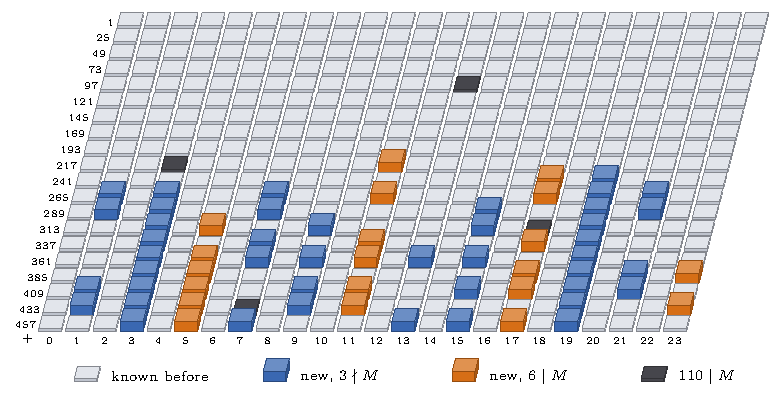
\includegraphics[width=\textwidth]{figures/fig_degrees}
\caption{The degrees $M\le480$, in rows of $24$: the row label plus the
column number is $M$. Light tiles are degrees covered by the results quoted
above, raised tiles are the degrees added by \Cref{thm:main}, and the dark
tiles are the multiples of $110$.}\label{fig:degrees}
\end{figure}

\subsection*{The method}
A Hodge line of $X^{4}_{M}$ is given by a \emph{sextuple}: six nonzero
residues modulo $M$, up to order, that are balanced in the sense of
\Cref{sec:fermat}. Three kinds of sextuples are known to give algebraic
lines: those that contain a pair $\{y,-y\}$, through the inductive structure
of Shioda and Katsura \cite{SK79}; the sextuples that split into two triples
with sum zero, through a product of two Fermat curves; and the standard
multisets of Aoki, through his explicit cycles \cite{Aok87}. A balanced
multiset that meets a standard multiset can be traded for the rest of it, and
we call such a trade a \emph{move}. The proof is an induction on the level and
on the orders of the entries: every sextuple without a pair has a chain of
moves to at most four elements, to a sextuple of smaller orders or to a split
sextuple, or it lies in one of finitely many explicit families, whose lines
we show to be algebraic directly.

The engine of the induction is a linear relation. If the largest order of an
entry of a sextuple $A$ is $e$, the balancing condition, read through Dirichlet
characters of conductor dividing $e$, says that the function counting the
entries of order $e$ in each residue class is a sum of functions that are
invariant under the subgroups $K_{p}$ of units congruent to $1$ modulo $e/p$,
one for each prime $p\mid e$ (\Cref{sec:primetosix}). Such \emph{split}
functions are rigid: a split function of small total mass is supported on a
single coset of one $K_{p}$, and a coset of $K_{p}$ is exactly what a move
needs. The only input from analytic number theory is the nonvanishing of the generalised
Bernoulli numbers $B_{1,\chi}$ for odd characters $\chi$.

\Cref{sec:fermat} recalls the description of the Hodge lines and the
algebraic tools, and \Cref{sec:primetosix} proves the rigidity of split
functions. \Cref{sec:odd} treats odd degrees. \Cref{sec:aoki} sets up Aoki's
reduction, and \Cref{sec:classes} supplies the classes it leaves at the
levels $33$, $35$, $39$, $44$, $52$, $102$ and $114$, by showing that the
relevant parts of the cohomology of Fermat threefolds are supported on
divisors. \Cref{sec:even,sec:four} treat even degrees prime to $3$, according
to the power of $2$ in the largest order of an entry, and \Cref{sec:six} the
degrees divisible by $6$. \Cref{sec:proof} assembles the proof.

\section{Fermat varieties and their Hodge characters}\label{sec:fermat}

\subsection{Correspondences}
All varieties are smooth and projective over $\CC$, possibly disconnected,
and cohomology has rational coefficients unless we say otherwise. Let $B$
and $X$ be varieties, with $B$ of pure dimension $b$. An algebraic cycle
$\Gamma$ of codimension $c$ on $B\times X$ gives the map
\[
  \Gamma_{*}\colon H^{k}(B)\to H^{k+2c-2b}(X),\qquad
  y\mapsto\pr_{X*}\bigl(\cl(\Gamma)\cup\pr_{B}^{*}y\bigr),
\]
a morphism of Hodge structures $H^{k}(B)(b-c)\to H^{k+2c-2b}(X)$. It carries
algebraic classes to algebraic classes, the composite of two such maps is the
map of the composite correspondence, and for a morphism $f\colon B\to X$ the
graph of $f$ and its transpose give $f_{*}$ and $f^{*}$
\cite[Chapter~16]{Ful98}.

A pure rational Hodge structure $V$ of weight $w$ is \emph{polarizable} if
it carries a bilinear form $Q$ with $Q(Cx,\bar x)>0$ for $x\ne0$, where $C$
acts on $V^{a,b}$ by $i^{a-b}$. The cohomology of a variety and its Tate
twists are polarizable \cite[Chapter~6]{Voi02b}, and polarizable Hodge
structures are semisimple.\footnote{If $W\subseteq V$ is a sub-Hodge
structure, the restriction of $Q$ to $W$ is again a polarization, so it is
nondegenerate and $V=W\oplus W^{\perp}$. The orthogonal $W^{\perp}$ is a
sub-Hodge structure, because $V_{\CC}=\bigoplus V^{a,b}$ is an orthogonal
decomposition for the hermitian form $Q(Cx,\bar y)$, and $W_{\CC}$ is the sum
of its intersections with the $V^{a,b}$.}

\begin{lemma}\label{lem:lift}
Let $\varphi\colon V\to W$ be a surjective morphism of polarizable Hodge
structures of weight $2p$. Then $\varphi$ maps the Hodge classes of $V$, the
rational classes of type $(p,p)$, onto those of $W$.
\end{lemma}

\begin{proof}
By semisimplicity the kernel of $\varphi$ has a complement $V'$ that is a
sub-Hodge structure, and $\varphi$ restricts to an isomorphism $V'\to W$ of
Hodge structures. Its inverse carries a Hodge class of $W$ to a Hodge class
of $V'\subseteq V$.
\end{proof}

\begin{theorem}[Lefschetz \cite{Lef24}, Kodaira--Spencer
\cite{KS53}]\label{thm:lef11}
Every Hodge class of degree two is algebraic.
\end{theorem}

\begin{proof}
In the exact sequence $H^{1}(X,\cO_{X}^{\times})\to H^{2}(X,\ZZ)\to
H^{2}(X,\cO_{X})$ of the exponential sequence, the second map is the
composite of $H^{2}(X,\ZZ)\to H^{2}(X,\CC)$ with the projection to
$H^{0,2}(X)$. So an integral class of type $(1,1)$ is the first Chern class
of a holomorphic line bundle, which is algebraic by GAGA, and its Chern class
is the class of a divisor. A rational Hodge class has an integral multiple.
\end{proof}

\subsection{The Fermat varieties}
For $m\ge1$ and $n\ge0$ let $X^{n}_{m}\subseteq\PP^{n+1}$ be the Fermat
variety $x_{0}^{m}+\dots+x_{n+1}^{m}=0$; thus $X^{0}_{m}$ is a set of $m$
points and $X^{1}_{m}$ the Fermat curve. The group
$G_{n}=\mu_{m}^{n+2}/\mu_{m}$ acts by multiplying the coordinates, and its
characters are the vectors $a=(a_{0},\dots,a_{n+1})\in(\ZZ/m)^{n+2}$ with
$\sum_{i}a_{i}=0$. Let $\mathfrak A^{n}_{m}$ be the set of characters with
every $a_{i}\ne0$. For $y\in\ZZ/m$ let $\bar y\in\{0,\dots,m-1\}$ be its
representative and $\langle y\rangle=\bar y/m$, and for
$a\in\mathfrak A^{n}_{m}$ put $\langle a\rangle=\sum_{i}\langle a_{i}\rangle$,
an integer between $1$ and $n+1$.

\begin{proposition}\label{prop:fermatchars}
\begin{enumerate}[label=\textup{(\roman*)}]
\item The primitive cohomology $H^{n}_{\mathrm{prim}}(X^{n}_{m},\CC)$ is the
direct sum of lines $V(a)$, $a\in\mathfrak A^{n}_{m}$, on which $G_{n}$ acts
by pull-back through the character $a$, and $V(a)\subseteq H^{n-q,q}$ with
$q=\langle a\rangle-1$.
\item Let $n$ be even. The space of primitive Hodge classes, tensored with
$\CC$, is the sum of the lines $V(a)$ with $\langle ta\rangle=n/2+1$ for
every $t\in(\ZZ/m)^{\times}$.
\end{enumerate}
\end{proposition}

\begin{proof}
(i) By Griffiths' description of the cohomology of a hypersurface by
residues \cite[\S8]{Gri69}, $H^{n-q,q}_{\mathrm{prim}}(X^{n}_{m})$ is
isomorphic to the graded piece of degree $(q+1)m-(n+2)$ of the Jacobian ring
$\CC[x_{0},\dots,x_{n+1}]/(x_{0}^{m-1},\dots,x_{n+1}^{m-1})$; the monomial
$x^{b}$ corresponds to the residue of $x^{b}\Omega/F^{q+1}$, where
$F=\sum x_{i}^{m}$ and $\Omega=\sum_{i}(-1)^{i}x_{i}\,dx_{0}\wedge\dots
\widehat{dx_{i}}\dots\wedge dx_{n+1}$. That residue is an eigenvector of
$G_{n}$ with character $a=b+(1,\dots,1)$, as $\Omega$ has character
$(1,\dots,1)$ and $F$ is invariant. As $b$ runs over the exponents with
$0\le b_{i}\le m-2$, $a$ runs once over the characters with all entries
nonzero, and the degree condition reads $\langle a\rangle=q+1$.

(ii) The decomposition is defined over $\QQ(\mu_{m})$, and the automorphism
$\zeta\mapsto\zeta^{t}$ of $\QQ(\mu_{m})$ carries $V(a)$ to $V(ta)$. So for
each orbit $O$ of $(\ZZ/m)^{\times}$ on $\mathfrak A^{n}_{m}$ the sum
$\bigoplus_{a\in O}V(a)$ is defined over $\QQ$, and these rational subspaces
decompose $H^{n}_{\mathrm{prim}}(X^{n}_{m},\QQ)$. A rational class with a
nonzero component on some $V(a)$ has nonzero components on the whole orbit of
$a$; so it is of type $(n/2,n/2)$ only if every $V(ta)$ is, that is, only if
$\langle ta\rangle=n/2+1$ for every unit $t$.
\end{proof}

\subsection{The inductive structure}
Fix $\varepsilon$ with $\varepsilon^{m}=-1$. For $r,s\ge1$, let
$Y\subseteq X^{r}_{m}\times X^{s}_{m}$ be the subvariety $x_{r+1}=y_{s+1}=0$,
which is isomorphic to $X^{r-1}_{m}\times X^{s-1}_{m}$, and let $Z$ be the
blow-up of $X^{r}_{m}\times X^{s}_{m}$ along $Y$. Shioda and Katsura show
that the rational map
\[
  (x,y)\mapsto\bigl[x_{0}y_{s+1}:\dots:x_{r}y_{s+1}:\varepsilon
  x_{r+1}y_{0}:\dots:\varepsilon x_{r+1}y_{s}\bigr]
\]
extends to a surjective morphism $\psi\colon Z\to X^{r+s}_{m}$
\cite[Lemma~1.2]{SK79}.\footnote{The image lies in $X^{r+s}_{m}$, because
$y_{s+1}^{m}\sum_{i\le r}x_{i}^{m}+\varepsilon^{m}x_{r+1}^{m}\sum_{j\le s}
y_{j}^{m}=-y_{s+1}^{m}x_{r+1}^{m}+x_{r+1}^{m}y_{s+1}^{m}=0$. All coordinates
vanish exactly on $Y$, and on the chart of the blow-up where
$y_{s+1}=t\,x_{r+1}$ the map is $[tx_{0}:\dots:tx_{r}:\varepsilon y_{0}:\dots:
\varepsilon y_{s}]$, where $y_{0},\dots,y_{s}$ do not all vanish.} Let
$E\subseteq Z$ be the exceptional divisor, $j\colon E\to Z$ the inclusion and
$\varpi\colon E\to Y$ the projection. The map
\[
  f=\psi_{*}j_{*}\varpi^{*}\colon H^{r+s-2}(Y)\to H^{r+s}(X^{r+s}_{m})
\]
carries $V(a')\otimes V(b')$ onto $V(a'*b')$ for $a'\in\mathfrak
A^{r-1}_{m}$ and $b'\in\mathfrak A^{s-1}_{m}$, where $a'*b'$ is the
juxtaposed character \cite[Theorem~II]{Shi79}, \cite[\S1]{Aok87}. As a
composite of pull-backs and push-forwards along morphisms, it carries
algebraic classes to algebraic classes.

\subsection{Balanced multisets}
In the rest of the paper $M\ge2$ is an integer, and we work with multisets
of elements of $\ZZ/M$; $A+B$ is the sum of multisets, $A-B$ the difference
when $B$ is contained in $A$, $tA$ and $-A$ the images under multiplication.

\begin{definition}\label{def:balanced}
Let $A$ be a multiset of nonzero elements of $\ZZ/M$ with sum $0$. It is
\emph{balanced} if $h_{A}(t)=\sum_{a\in A}\langle ta\rangle$ is the same
integer for every $t\in(\ZZ/M)^{\times}$. A \emph{pair} is a submultiset
$\{a,-a\}$; when $M$ is even, $\{M/2,M/2\}$ is a pair. A multiset is
\emph{split} if it is the sum of two multisets of three elements, each with
sum $0$.
\end{definition}

Comparing $t$ with $-t$ shows that a balanced multiset of $n$ elements has
$h_{A}=n/2$, so $n$ is even. Ordering the elements of a balanced multiset of
$n\ge2$ elements gives a character $\alpha\in\mathfrak A^{n-2}_{M}$, and by
\Cref{prop:fermatchars}(ii) the line $V(\alpha)$ consists of Hodge classes
(for $n=2$, $X^{0}_{M}$ is a set of $M$ points). Permuting the coordinates
permutes these lines, so the following notion does not depend on the order:
$A$ is \emph{algebraic} if $V(\alpha)\subseteq\Alg^{(n-2)/2}(X^{n-2}_{M})
\otimes\CC$. Conversely every Hodge class of $X^{4}_{M}$ is, over $\CC$, a
sum of a multiple of the square of the hyperplane class and of vectors of
lines $V(\alpha)$ with $\alpha$ balanced. Since $\Alg^{2}\subseteq\Hdg^{2}$
are rational subspaces, this gives:

\begin{lemma}\label{lem:reducetosextuples}
The Hodge conjecture holds for $X^{4}_{M}$ if and only if every balanced
multiset of six nonzero elements of $\ZZ/M$ is algebraic.
\end{lemma}

A balanced multiset of six nonzero elements is a \emph{sextuple at level
$M$}.

For an odd prime $\ell\mid M$ and $x\in\ZZ/M$ put
$\Phi_{\ell}(x)=\{x+jM/\ell:\ 0\le j<\ell\}$, the solutions $y$ of
$\ell y=\ell x$, and
\[
  \sigma_{\ell,x}=\Phi_{\ell}(x)+\{-\ell x\}.
\]
For even $M$ and $x\in\ZZ/M$ with $2x\ne0$ put
\[
  T(x)=\{x,\ x+M/2,\ -2x,\ M/2\}.
\]
These are the \emph{standard multisets} of Aoki \cite[\S1]{Aok87}.

\begin{lemma}\label{lem:algtools}
Let $A$ and $B$ be balanced multisets of nonzero elements of $\ZZ/M$.
\begin{enumerate}[label=\textup{(\alph*)}]
\item If $|A|\le4$, then $A$ is algebraic.
\item If $A$ and $B$ are algebraic, so is $A+B$. If $P$ is a sum of pairs and
$A+P$ is algebraic, then $A$ is algebraic.
\item For a unit $t$, $tA$ is balanced, and it is algebraic if and only if
$A$ is.
\item Let $g\mid M$, $M'=M/g$, let $A'$ be a multiset of nonzero elements of
$\ZZ/M'$ with sum $0$, and let $gA'\subseteq\ZZ/M$ be its image under
$y\mapsto gy$. Then $gA'$ is balanced if and only if $A'$ is, and in that
case $gA'$ is algebraic if and only if $A'$ is.
\item If $\ell x\ne0$, then $\sigma_{\ell,x}$ is balanced and algebraic. If
$M$ is even and $2x\ne0$, then $T(x)$ is balanced and algebraic.
\item A split sextuple is algebraic.
\end{enumerate}
\end{lemma}

\begin{proof}
(a) For $|A|=2$, $A=\{a,-a\}$ and $H^{0}(X^{0}_{M})$ is spanned by classes of
points. For $|A|=4$, $V(\alpha)$ consists of Hodge classes of degree two on
the surface $X^{2}_{M}$, which are algebraic by \Cref{thm:lef11}.

(b) The line of $A+B$ is the image of $V(\alpha)\otimes V(\beta)$ under the
map $f$ of the inductive structure, which preserves algebraic classes; this
is \cite[Theorem~1-4]{Aok87}, which also gives the converse for a pair
$\{a,-a\}$, whose line on $X^{0}_{M}$ is spanned by a class of points.

(c) The automorphism $\zeta\mapsto\zeta^{t}$ of $\QQ(\mu_{M})$, acting on
$H^{*}(X^{n-2}_{M},\QQ)\otimes\QQ(\mu_{M})$ through the second factor,
carries $V(\alpha)$, which is defined over $\QQ(\mu_{M})$, onto $V(t\alpha)$,
and preserves $\Alg\otimes\QQ(\mu_{M})$.

(d) Every unit modulo $M'$ lifts to a unit modulo $M$, and
$\langle tgy\rangle=\langle t'y\rangle$ for $y\in\ZZ/M'$ and a unit $t$ with
image $t'$, the first bracket taken modulo $M$ and the second modulo $M'$;
this gives the first assertion. Let $\pi\colon X^{n-2}_{M}\to X^{n-2}_{M'}$
be the finite morphism $[x_{i}]\mapsto[x_{i}^{g}]$, of degree
$g^{n-1}$. It is equivariant for the homomorphism $G\to G'$,
$\zeta\mapsto\zeta^{g}$, so for $\xi\in V(\alpha')$ and $\zeta\in G$,
$\zeta^{*}\pi^{*}\xi=\pi^{*}(\zeta^{g})^{*}\xi=\alpha'(\zeta^{g})\pi^{*}\xi$,
and $\pi^{*}V(\alpha')\subseteq V(g\alpha')$. Since $\pi_{*}\pi^{*}$ is
multiplication by $\deg\pi$, $\pi^{*}$ is injective, and as both are lines,
$\pi^{*}V(\alpha')=V(g\alpha')$ and $V(\alpha')=\pi_{*}V(g\alpha')$. Both
$\pi^{*}$ and $\pi_{*}$ preserve algebraic classes.

(e) The elements of $\Phi_{\ell}(x)$ are nonzero since $\ell x\ne0$, and the
sum of $\sigma_{\ell,x}$ is $\ell x+\binom{\ell}{2}M/\ell-\ell x=0$, as $\ell$
is odd. For a unit $t$, $t\Phi_{\ell}(x)=\Phi_{\ell}(tx)$, and writing
$\overline{tx}=qM/\ell+r$ with $0\le r<M/\ell$,
\[
  \sum_{y\in\Phi_{\ell}(tx)}\bar y=\sum_{j=0}^{\ell-1}\Bigl(\bigl((q+j)\bmod
  \ell\bigr)\frac{M}{\ell}+r\Bigr)=\frac{(\ell-1)M}{2}+\overline{\ell tx};
\]
adding $\overline{-\ell tx}=M-\overline{\ell tx}$ gives $(\ell+1)M/2$, so
$\sigma_{\ell,x}$ is balanced. For $\ell=3$ it is algebraic by (a). Let
$\ell\ge5$, $d=M/\ell$, and let $i$ be the representative of $x$ in
$\{1,\dots,d-1\}$ modulo $d$ (it is not $0$, as $\ell x\ne0$); then
$\Phi_{\ell}(x)=\Phi_{\ell}(i)$ and $\ell x=\ell i$. Put $g=\gcd(i,d)$,
$M'=M/g$, $d'=d/g$, $i'=i/g$. Then $\sigma_{\ell,x}=g\,\sigma_{\ell,i'}$ with
$\sigma_{\ell,i'}$ formed at level $M'$, and $\gcd(i',d')=1$, $d'\ge2$. If
$d'\ge3$, Aoki constructs a subvariety of $X^{\ell-1}_{M'}$ of codimension
$(\ell-1)/2$ that represents $\sigma_{\ell,i'}$ \cite[Theorem~2-1]{Aok87}, so
$\sigma_{\ell,i'}$ is algebraic. If $d'=2$, then $i'=1$, $M'=2\ell$, and
$\sigma_{\ell,1}=\{1,3,\dots,2\ell-1\}+\{\ell\}$ is the sum of the pairs
$\{y,2\ell-y\}$, $y<\ell$ odd, and $\{\ell,\ell\}$, algebraic by (a) and (b).
In both cases (d) gives the claim.

For $T(x)$: let $t$ be a unit, which is odd, and $y=\overline{tx}$; then
$y\ne M/2$ and $tM/2=M/2$. The representatives of the elements of $tT(x)$
are $y,\ y+M/2,\ M-2y,\ M/2$ if $y<M/2$, and $y,\ y-M/2,\ 2M-2y,\ M/2$ if
$y>M/2$; both add up to $2M$. So $T(x)$ is balanced, and it is algebraic by
(a).

(f) Let $A=A_{1}+A_{2}$ with $|A_{i}|=3$ and sums $0$. Their elements are
nonzero, and the entries of $A_{1}$ and $A_{2}$ are characters $a'$ and $b'$
of the Fermat curve $X^{1}_{M}$, with $\langle ta'\rangle,\langle
tb'\rangle\in\{1,2\}$ and $\langle ta'\rangle+\langle tb'\rangle=3$ for every
unit $t$. So $V(ta')\otimes V(tb')$ has type $(1,1)$ in
$H^{2}(X^{1}_{M}\times X^{1}_{M})$, and the sum $L$ of these lines over the
units is stable under $\operatorname{Gal}(\QQ(\mu_{M})/\QQ)$, so
$L=L_{\QQ}\otimes\CC$ for a space $L_{\QQ}$ of Hodge classes of degree two on
the surface $X^{1}_{M}\times X^{1}_{M}$. They are algebraic by
\Cref{thm:lef11}, and $f$ with $r=s=2$ carries $V(a')\otimes V(b')$ onto the
line of $A$.
\end{proof}

\subsection{Moves}
The proofs below replace a sextuple by another multiset in a way that keeps
track of algebraicity.

\begin{definition}\label{def:move}
Let $A$ be a balanced multiset of nonzero elements, $\sigma$ an algebraic
balanced multiset, and $S\subseteq A$ a submultiset that is also contained in
$\sigma$. The multiset
\[
  A''=(A-S)+\bigl(-(\sigma-S)\bigr)
\]
is the result of the \emph{move} $(\sigma,S)$. We usually take $\sigma$
standard, $S$ consisting of the elements of $A$ that lie in $\sigma$, and
we remove from $A''$ every pair it contains.
\end{definition}

\begin{lemma}\label{lem:move}
In \Cref{def:move}, $A''$ is a balanced multiset of nonzero elements and
$A''+\sigma=A+P$ for a sum of pairs $P$. If $A''$ is algebraic, so is $A$.
The same holds for a chain of moves.
\end{lemma}

\begin{proof}
With $P=(\sigma-S)+(-(\sigma-S))$ we have $A''+\sigma=(A-S)+S+(\sigma-S)+
(-(\sigma-S))=A+P$. The sum and the function $h$ are additive, and $A$, $P$,
$\sigma$ are balanced; so $A''$ is balanced. If $A''$ is algebraic, then
$A+P=A''+\sigma$ is algebraic by \Cref{lem:algtools}(b), and so is $A$.
\end{proof}

The \emph{profile} $o(A)$ of a sextuple is the sequence of the additive
orders of its elements in nonincreasing order, and profiles are compared
lexicographically. For two sextuples $A$ and $A''$, $o(A'')<o(A)$ exactly when,
at the largest integer $f$ at which $A$ and $A''$ have different numbers of
elements of order $f$, $A$ has more. A chain of moves that turns a sextuple
$A$ into a multiset $A^{\flat}$ with at most four elements is \emph{direct};
it is \emph{lowering} if $A^{\flat}$ is a sextuple with $o(A^{\flat})<o(A)$;
it \emph{succeeds} if it is direct or lowering, or $A^{\flat}$ is a split
sextuple, or a sextuple that lies in a proper subgroup of $\ZZ/M$.

\begin{proposition}[Induction]\label{prop:induction}
Let $M\ge2$, and suppose that the Hodge conjecture holds for $X^{4}_{M'}$
for every proper divisor $M'$ of $M$. Suppose that every sextuple at level
$M$ that contains no pair, is not split and generates $\ZZ/M$ has a chain of
moves that succeeds, or is algebraic for another reason. Then the Hodge
conjecture holds for $X^{4}_{M}$.
\end{proposition}

\begin{proof}
By \Cref{lem:reducetosextuples} we show that every sextuple $A$ at level $M$
is algebraic, by induction on the profile, which takes finitely many values.
If $A$ contains a pair, then removing it leaves a balanced multiset of four
elements, and $A$ is algebraic by \Cref{lem:algtools}(a),(b). If $A$ is split,
\Cref{lem:algtools}(f) applies. If $A$ lies in the subgroup $g\ZZ/M$, $g>1$,
then $A=gA'$ for a sextuple $A'$ at level $M/g$, which is algebraic by
\Cref{lem:reducetosextuples} and the hypothesis, and so is $A$ by
\Cref{lem:algtools}(d). Otherwise $A$ has a chain of moves that succeeds, or
is algebraic by assumption. In the first case the last multiset $A^{\flat}$
is algebraic by \Cref{lem:algtools}(a), by induction on the profile, or by
the cases already treated, and $A$ is algebraic by \Cref{lem:move}.
\end{proof}

\section{Degrees prime to six}\label{sec:primetosix}

In this section $M$ is prime to $6$. For $x\in\ZZ/M$ with $5\mid M$ we write
$\Phi(x)=\Phi_{5}(x)$, so that $\sigma_{5,x}=\Phi(x)+\{-5x\}$.

\begin{theorem}\label{thm:sextuples}
Let $M$ be prime to $6$.
\begin{enumerate}[label=\textup{(\roman*)}]
\item Every balanced multiset of four nonzero elements of $\ZZ/M$ contains a
pair.
\item Every balanced multiset of six nonzero elements of $\ZZ/M$ contains a
pair or is $\sigma_{5,x}$ for some $x$ with $5x\ne0$.
\end{enumerate}
\end{theorem}

Part (i) is Aoki's theorem that the Hodge classes of a Fermat surface of
degree prime to $6$ are spanned by classes of lines \cite[Theorem~A]{Aok83};
we prove it again because the proof of (ii) uses it and runs on the same
lines. When $5\nmid M$, every prime factor of $M$ exceeds $6$, and (ii) is
also contained in \cite[Theorem~A]{Aok83}.

\begin{corollary}\label{cor:primetosix}
The Hodge conjecture holds for $X^{4}_{M}$ when $M$ is prime to $6$.
\end{corollary}

\begin{proof}
By \Cref{lem:reducetosextuples} it suffices to show that every sextuple $A$ at
level $M$ is algebraic. If $A=A'+\{a,-a\}$, then $A'$ is balanced, because
$\langle ta\rangle+\langle-ta\rangle=1$ for every unit $t$; it has four
elements and is algebraic by \Cref{lem:algtools}(a), and $A$ is algebraic by
\Cref{lem:algtools}(b). Otherwise $A=\sigma_{5,x}$ with $5x\ne0$ by
\Cref{thm:sextuples}(ii), and \Cref{lem:algtools}(e) applies.
\end{proof}

The rest of this section proves \Cref{thm:sextuples}. We fix a balanced
multiset $A$ of $n\in\{4,6\}$ nonzero elements of $\ZZ/M$ that contains no
pair, and show that $n=6$ and that $A$ is a multiset $\sigma_{5,x}$. Since $A$
is balanced, $\sum_{a\in A}\overline{ta}=nM/2$ for every unit $t$.

\subsection{The counting function}
Let $e$ be the largest additive order of an element of $A$. It divides $M$,
so it is prime to $6$, and $e>1$. The map $\kappa\colon\ZZ/e\to\ZZ/M$,
$y\mapsto(M/e)y$, is an injective homomorphism, and the elements of $\ZZ/M$
of order exactly $e$ are the $\kappa(z)$ with $z\in U=(\ZZ/e)^{\times}$. For
$z\in U$ put
\[
  F(z)=\mult_{A}(\kappa z)-\mult_{A}(-\kappa z),
\]
the difference of the multiplicities in $A$. Then $F(-z)=-F(z)$. If
$a_{0}=\kappa(z_{0})\in A$ has order $e$, then $-a_{0}\notin A$, so
$F(z_{0})\ge1$. We call $\|F\|=\sum_{z\in U}|F(z)|$ the \emph{mass} of $F$.

\begin{lemma}\label{lem:countF}
$\|F\|\le2n$. If $\|F\|=2n$, then every element of $A$ has order $e$ and
$\sum_{z\in U}F(z)\,z=0$ in $\ZZ/e$.
\end{lemma}

\begin{proof}
$\|F\|\le\sum_{z}(\mult_{A}(\kappa z)+\mult_{A}(-\kappa z))=2N$, where
$N\le n$ is the number of elements of $A$ of order $e$. If $\|F\|=2n$, then
$N=n$, and writing $a=\kappa(z_{a})$ for $a\in A$,
\[
  \sum_{z}F(z)z=\sum_{a\in A}z_{a}-\sum_{a\in A}(-z_{a})=2\sum_{a\in
  A}z_{a},
\]
while $\kappa(\sum_{a}z_{a})=\sum_{a}a=0$; as $\kappa$ is injective,
$\sum_{a}z_{a}=0$.
\end{proof}

\subsection{The characters}
For a Dirichlet character $\chi$ modulo $e$ let $B_{1,\chi}=e^{-1}\sum_{s=1}
^{e}\chi(s)s$. If $\chi$ is odd and primitive, then $B_{1,\chi}\ne0$: it is a
nonzero multiple of $L(1,\bar\chi)$ \cite[Theorem~4.9]{Was97}, and
$L(1,\bar\chi)\ne0$.\footnote{The relative class number formula
\cite[Theorem~4.17]{Was97} expresses the relative class number of
$\QQ(\mu_{e})$, a positive integer, as a nonzero rational multiple of the
product of the numbers $-B_{1,\chi}/2$ over the odd characters $\chi$; so no
factor vanishes. This is the only analytic input of the proof.}

\begin{lemma}\label{lem:charstep}
$\sum_{z\in U}F(z)\chi(z)^{-1}=0$ for every primitive Dirichlet character
$\chi$ modulo $e$.
\end{lemma}

\begin{proof}
If $\chi$ is even, the sum vanishes because $F$ is odd. Let $\chi$ be odd,
and regard it as a character of $(\ZZ/M)^{\times}$ through reduction modulo
$e$; it is not trivial. Since $A$ is balanced,
\[
  \sum_{a\in A}\ \sum_{t\in(\ZZ/M)^{\times}}\chi(t)\,\overline{ta}
  =\frac{nM}{2}\sum_{t}\chi(t)=0.
\]
Let $a\in A$ have order $f$. If $f\ne e$, then $e\nmid f$, since $f\le e$.
For a divisor $f$ of $M$ let $W_{f}\subseteq(\ZZ/M)^{\times}$ be the units
congruent to $1$ modulo $f$. If $\chi$ were trivial on $W_{f}$, it would be
trivial on $W_{f}W_{e}=W_{\gcd(f,e)}$ by the Chinese remainder theorem, so it
would be induced from a character modulo the proper divisor $\gcd(f,e)$ of
$e$, against primitivity. So $\chi$ is not trivial on $W_{f}$; as
$\overline{ta}$ depends only on $t$ modulo $f$, the inner sum vanishes. If
$f=e$, write $a=\kappa(z)$. For a unit $t$ with image $s\in U$ we have
$ta=\kappa(sz)$ and $\overline{ta}=(M/e)\,\overline{sz}$, where now
$\overline{sz}\in\{0,\dots,e-1\}$. Reduction $(\ZZ/M)^{\times}\to U$ is onto,
with fibres of size $\varphi(M)/\varphi(e)$, so
\[
  \sum_{t}\chi(t)\,\overline{ta}=\frac{M\,\varphi(M)}{e\,\varphi(e)}
  \sum_{s\in U}\chi(s)\,\overline{sz}=\frac{M\,\varphi(M)}{\varphi(e)}\,
  \chi(z)^{-1}B_{1,\chi},
\]
after the substitution $s\mapsto sz^{-1}$. Adding over $A$ and dividing by
$M\varphi(M)B_{1,\chi}/\varphi(e)\ne0$ gives $\sum_{z}\mult_{A}(\kappa z)
\chi(z)^{-1}=0$. The substitution $z\mapsto-z$ turns
$\sum_{z}\mult_{A}(-\kappa z)\chi(z)^{-1}$ into $\chi(-1)^{-1}$ times the
same sum, so it vanishes too, and so does their difference.
\end{proof}

\subsection{Splitting along the subgroups \texorpdfstring{$K_{p}$}{K\_p}}
For a prime $p\mid e$ let $K_{p}\subseteq U$ be the subgroup of units
congruent to $1$ modulo $e/p$, the kernel of $U\to(\ZZ/(e/p))^{\times}$.

\begin{lemma}\label{lem:Kp}
\begin{enumerate}[label=\textup{(\alph*)}]
\item $|K_{p}|=p$ if $p^{2}\mid e$, and $|K_{p}|=p-1$ if $p\parallel e$. So
$|K_{p}|\ge4$, with equality only for $p=5\parallel e$.
\item Let $p^{v}\parallel e$. The product of the $K_{q}$ with $q\ne p$
consists of units congruent to $1$ modulo $p^{v}$. Hence $K_{p}$ meets it
trivially, the product $H$ of all the $K_{q}$ is direct, and $-1$ does not
lie in the product of the $K_{q}$ with $q\ne p$.
\item A Dirichlet character modulo $e$ that is not primitive is trivial on
some $K_{p}$.
\end{enumerate}
\end{lemma}

\begin{proof}
(a) $|K_{p}|=\varphi(e)/\varphi(e/p)$. (b) For $q\ne p$, $p^{v}$ divides
$e/q$. An element of $K_{p}$ congruent to $1$ modulo $p^{v}$ is congruent to
$1$ modulo $\lcm(e/p,p^{v})=e$, and $-1\not\equiv1\pmod p$ as $p$ is odd.
(c) A character induced from a proper divisor $f$ of $e$ is trivial on the
units congruent to $1$ modulo $f$, and $f$ divides $e/p$ for some $p\mid e$.
\end{proof}

\begin{definition}\label{def:split}
Let $K_{1},\dots,K_{r}$ be subgroups of a finite abelian group, $H$ their
product and $C$ a coset of $H$. A function $f\colon C\to\ZZ$ is \emph{split
along} $(K_{1},\dots,K_{r})$ if $f=f_{1}+\dots+f_{r}$ with functions
$f_{i}\colon C\to\CC$ such that $f_{i}(zk)=f_{i}(z)$ for $z\in C$ and $k\in
K_{i}$; for $r=0$ this means $f=0$. A \emph{line} along $K_{i}$ is a coset
$wK_{i}$.
\end{definition}

\begin{lemma}\label{lem:splitF}
On every coset of $H$ in $U$, the function $F$ is split along the family
$(K_{p})_{p\mid e}$.
\end{lemma}

\begin{proof}
By Fourier inversion on $U$, $F=\varphi(e)^{-1}\sum_{\chi}\hat F(\chi)\chi$
with $\hat F(\chi)=\sum_{z}F(z)\chi(z)^{-1}$. By \Cref{lem:charstep} only
characters that are not primitive contribute, and by \Cref{lem:Kp}(c) each of
them is trivial on some $K_{p}$. Collect the terms according to such a $p$.
\end{proof}

Four properties of split functions are used below, for $f$ split along
$(K_{1},\dots,K_{r})$ on $C$ and $H'=K_{2}\cdots K_{r}$.
\begin{enumerate}[label=\textup{(S\arabic*)}]
\item For $k\in K_{1}$ and every coset $S\subseteq C$ of $H'$, the function
$z\mapsto f(z)-f(zk)$ on $S$ is split along $(K_{2},\dots,K_{r})$: the terms
$f_{1}$ cancel.
\item If $f$ vanishes on one coset $S_{0}\subseteq C$ of $H'$, then $f$ is
split along $(K_{2},\dots,K_{r})$ on every coset $S\subseteq C$ of $H'$:
choose $k\in K_{1}$ with $Sk=S_{0}$ and apply (S1).
\item For $r=2$ and $C=xK_{1}K_{2}$: $f(xij)=f(xi)+f(xj)-f(x)$ for $i\in
K_{1}$ and $j\in K_{2}$.
\item For $r=1$, $f$ is invariant under $K_{1}$.
\end{enumerate}

\subsection{Three lemmas on split functions}
In the next three lemmas, $K_{1},\dots,K_{r}$ are subgroups of a finite
abelian group whose product $H$ is direct (the first one is sometimes called
$K$), and $C$ is a coset of $H$. Fix $x\in C$ and put $H'=K_{2}\cdots K_{r}$. For $c$ in the
first subgroup, the \emph{slices} of $C$ are the cosets $S_{c}=xcH'$; they
are pairwise distinct, and for a function $f$ on $C$ we write
$\mu(c)=\sum_{z\in S_{c}}|f(z)|$.

\begin{lemma}\label{lem:grid}
Suppose $|K_{i}|\ge4$ for every $i$, with equality for at most one $i$. Let
$f\colon C\to\ZZ$ be split along $(K_{1},\dots,K_{r})$, not identically zero,
with $\sum_{C}|f|\le6$. Then for some $i$ with $|K_{i}|\le6$ there are a line
$L=wK_{i}\subseteq C$ and $\sigma\in\{\pm1\}$ such that $f=\sigma$ on $L$ and
$f=0$ on $C\setminus L$.
\end{lemma}

\begin{proof}
Induction on $r$. For $r=0$ the function vanishes, which is excluded. Let
$r\ge1$ and $K=K_{1}$. First an observation.

(P) \emph{Let $c,c'\in K$ with $\mu(c)+\mu(c')\le6$, and suppose
$g(z)=f(z)-f(zc^{-1}c')$ is not identically zero on $S_{c}$. Then
$\mu(c)+\mu(c')\ge|K_{i}|$ for some $i\ge2$.} Indeed, $g$ is split along
$(K_{2},\dots,K_{r})$ on $S_{c}$ by (S1), and $\sum_{S_{c}}|g|\le\mu(c)+
\mu(c')$ because $z\mapsto zc^{-1}c'$ maps $S_{c}$ onto $S_{c'}$. By
induction $|g|$ is $1$ on a line along some $K_{i}$, $i\ge2$, and $0$
elsewhere, so $\sum_{S_{c}}|g|=|K_{i}|$.

\emph{Case A: $f(zk)=f(z)$ for all $z\in C$, $k\in K$.} Let $f(z_{0})\ne0$.
Then $f$ equals $f(z_{0})$ on the $|K|\ge4$ points of $z_{0}K$, so
$|f(z_{0})|=1$ and $|K|\le6$, and a nonzero value off $z_{0}K$ would add at
least $|K|\ge4$ more. So $f=f(z_{0})$ on $z_{0}K$ and $0$ elsewhere.

\emph{Case B1: $\mu(c_{0})=0$ for some $c_{0}$.} By (S2), $f$ is split along
$(K_{2},\dots,K_{r})$ on every slice. On a slice where it does not vanish, by
induction it is $\pm1$ on a line along some $K_{i}$ with $i\ge2$ and
$|K_{i}|\le6$ and $0$ elsewhere, which uses mass $|K_{i}|\ge4$; a second such
slice would bring the mass to $8$. This is the claim.

\emph{Case B2: $f$ is not $K$-invariant, and $\mu\ge1$ on every slice.} As
$\sum\mu\le6<2|K|$, some $c_{s}$ has $\mu(c_{s})=1$. Choose $c,k\in K$ such
that $f(z)\ne f(zk)$ for some $z\in S_{c}$. By (P), applied to $c$ and $ck$,
or because $\mu(c)+\mu(ck)>6$, one of them, $c_{1}$, has $\mu(c_{1})\ge2$.
Then $f(z)-f(zc_{1}^{-1}c_{s})$ does not vanish identically on $S_{c_{1}}$,
since translation carries $S_{c_{1}}$ onto $S_{c_{s}}$ and $\mu(c_{1})\ne
\mu(c_{s})$. By (P), $\mu(c_{1})+1\ge|K_{i}|\ge4$ for some $i\ge2$, so
\[
  6\ge\sum_{c\in K}\mu(c)\ge\mu(c_{1})+(|K|-1)\ge3+3.
\]
All these are equalities: $|K|=4$ and $|K_{i}|=\mu(c_{1})+1=4$, two
subgroups of order four, which is excluded.
\end{proof}

\begin{lemma}\label{lem:oddbig}
Let $|K|\ge10$ and $|K_{i}|\ge4$ for $i\ge2$, with equality for at most one
$i$. Let $f\colon C\to\ZZ$ be split along $(K,K_{2},\dots,K_{r})$, and suppose
that for some $\varepsilon\in K\setminus\{1\}$ and $\varepsilon'\in H'$ we
have $f(z\varepsilon\varepsilon')=-f(z)$ for all $z\in C$. If $\sum_{C}|f|
\le12$ and $f(x)\ge1$, then $f=1$ on a line along some $K_{i}$, $i\ge2$, with
$|K_{i}|\le6$.
\end{lemma}

\begin{proof}
Multiplication by $\varepsilon\varepsilon'$ carries $S_{c}$ onto
$S_{c\varepsilon}$ and preserves $|f|$, so $\mu(c\varepsilon)=\mu(c)$. If
some slice has $\mu=0$, then $f$ is split along $(K_{2},\dots,K_{r})$ on
$S_{1}\ni x$ by (S2), and $2\mu(1)=\mu(1)+\mu(\varepsilon)\le12$; by
\Cref{lem:grid}, $f$ is $\sigma$ on a line along some $K_{i}$ in $S_{1}$ and
$0$ elsewhere on $S_{1}$, and $\sigma=1$ because the line passes through $x$.
Otherwise $\mu\ge1$ everywhere, and as $\sum\mu\le12<2|K|$, some $c$ has
$\mu(c)=1$, hence $\mu(c\varepsilon)=1$. The function $f(z)-f(z\varepsilon)$
on $S_{c}$ is split along $(K_{2},\dots,K_{r})$ by (S1) and has mass at most
$2$, so it vanishes by \Cref{lem:grid}. Let $z_{0}$ be the point of $S_{c}$
with $f(z_{0})=\pm1$. The points $z_{0}\varepsilon$ and
$z_{0}\varepsilon\varepsilon'$ of $S_{c\varepsilon}$ carry the values
$f(z_{0})$ and $-f(z_{0})$, both nonzero, so they coincide because
$\mu(c\varepsilon)=1$; then $f(z_{0})=-f(z_{0})$, a contradiction.
\end{proof}

\begin{lemma}\label{lem:twoD}
Let $K\cap L=1$, $|K|=4$, $|L|=6$, and let $\varepsilon\in K$ and
$\varepsilon'\in L$ be different from $1$, with $\varepsilon^{2}=1$. Let
$f\colon xKL\to\ZZ$ be split along $(K,L)$, with $f(z\varepsilon
\varepsilon')=-f(z)$, $\sum|f|\le12$ and $f(x)\ge1$. Then
\begin{enumerate}[label=\textup{(\alph*)}]
\item $f(xi)=1$ for all $i\in K$; or
\item $f(xj)=1$ for all $j\in L$; or
\item $\sum|f|=12$, and there are $u\colon K\to\{\pm1\}$ and $v\colon
L\to\{\pm1\}$ with $u(i\varepsilon)=-u(i)$, $v(j\varepsilon')=-v(j)$ and
$2f(xij)=u(i)+v(j)$.
\end{enumerate}
\end{lemma}

\begin{proof}
By (S3), $f(xij)=f(xi)+f(xj)-f(x)$. Put $\delta=f(x)-f(x\varepsilon')$,
$u(i)=2f(xi)-\delta$ and $v(j)=2f(xj)-2f(x)+\delta$, so that $2f(xij)=u(i)+
v(j)$. Comparing $f(xi\varepsilon\cdot\varepsilon')=-f(xi)$ with (S3) gives
$f(xi\varepsilon)+f(xi)=\delta$, that is $u(i\varepsilon)=-u(i)$; for $i=1$
it gives $f(x\varepsilon)=-f(x\varepsilon')$, and then the same comparison
for $x\varepsilon\cdot j\varepsilon'$ gives $v(j\varepsilon')=-v(j)$. Since
$j\mapsto j\varepsilon'$ permutes $L$ and changes the sign of $v$,
\[
  2\sum_{j}|u(i)+v(j)|=\sum_{j}\bigl(|u(i)+v(j)|+|u(i)-v(j)|\bigr)
  =2\sum_{j}\max(|u(i)|,|v(j)|),
\]
so $T=\sum_{i,j}\max(|u(i)|,|v(j)|)=2\sum|f|\le24$. All $u(i)$ and $v(j)$
have the same parity, because $u(i)+v(j)=2f(xij)$. Write
$K=\{1,\varepsilon,a,a\varepsilon\}$, $V=\sum_{j}|v(j)|$ and
$\Sigma(s)=\sum_{j}\max(s,|v(j)|)$; then $T=2\Sigma(|u(1)|)+2\Sigma(|u(a)|)$,
$\Sigma(s)\ge\max(6s,V)$, and $V\ge2|v(1)|$ because
$|v(\varepsilon')|=|v(1)|$.

If the parity is odd, all $24$ terms of $T$ are at least $1$, so all equal
$1$, and we are in case (c). If it is even and $u(1)\ge1$, then $u(1)\ge2$
and $24\ge T\ge24+2V$, so $u(1)=2$, $v=0$, and $f(xj)=(u(1)+v(j))/2=1$: case
(b). If it is even and $u(1)\le0$, then $v(1)=2f(x)-u(1)\ge2$. If $u(1)\ne0$,
then $T\ge2\cdot12+2V>24$; so $u(1)=0$, and in the same way $u(a)=0$. Then
$u=0$ on $K$, $T=4V\le24$, so $2v(1)\le V\le6$ and $v(1)=2$, and
$f(xi)=(u(i)+v(1))/2=1$: case (a).
\end{proof}

\subsection{The core dichotomy}

\begin{proposition}\label{prop:core}
Let $e>1$ be prime to $6$, $U=(\ZZ/e)^{\times}$, and let $F\colon U\to\ZZ$
satisfy $F(-z)=-F(z)$, $\|F\|\le12$ and $F(x)\ge1$ for some $x$, and be split
along $(K_{p})_{p\mid e}$ on every coset of their product $H$. Then
\begin{enumerate}[label=\textup{(\arabic*)}]
\item $F\ge1$ on a line $wK_{p}$ for $p=5$ or $p=7$; or
\item the primes dividing $e$ are $5$ and $7$, $|K_{5}|=4$, $|K_{7}|=6$, and
there are $y\in U$, $\varepsilon\in K_{5}$ and $\varepsilon'\in K_{7}$ with
$\varepsilon\varepsilon'=-1$, and functions $u\colon K_{5}\to\{\pm1\}$ and
$v\colon K_{7}\to\{\pm1\}$ with $u(i\varepsilon)=-u(i)$,
$v(j\varepsilon')=-v(j)$ and $2F(yij)=u(i)+v(j)$ for $i\in K_{5}$, $j\in
K_{7}$; the mass of $F$ on $yK_{5}K_{7}$ is $12$.
\end{enumerate}
\end{proposition}

\begin{proof}
By \Cref{lem:Kp}(a) every $|K_{p}|$ is at least $4$, only $K_{5}$ can have
order $4$, and $|K_{p}|\le9$ forces $p\in\{5,7\}$.

\emph{Case (a): $-1\notin H$.} The cosets $xH$ and $-xH$ are distinct and
carry the same mass, so $\sum_{xH}|F|\le6$. By \Cref{lem:grid}, $F=\sigma$ on
a line along some $K_{p}$ with $|K_{p}|\le6$, so $p\in\{5,7\}$, and
$\sigma=1$ because the line passes through $x$.

\emph{Case (b): $-1\in H$ and $|K_{p}|\ge10$ for some $p$.} Write
$-1=\varepsilon\varepsilon'$ with $\varepsilon\in K_{p}$ and $\varepsilon'$
in the product of the other $K_{q}$; $\varepsilon\ne1$ by \Cref{lem:Kp}(b).
\Cref{lem:oddbig} gives (1).

\emph{Case (c): $-1\in H$ and $|K_{p}|\le9$ for all $p$.} Then every prime
factor of $e$ is $5$ or $7$. If only one prime $p$ divides $e$, then $-1\in
K_{p}$ and $F$ is $K_{p}$-invariant on $xK_{p}$ by (S4), so
$F(x)=F(-x)=-F(x)$, which is impossible. So $H=K_{5}K_{7}$, and
$-1=\varepsilon\varepsilon'$ with $\varepsilon\in K_{5}$, $\varepsilon'\in
K_{7}$, both different from $1$ by \Cref{lem:Kp}(b). From
$\varepsilon^{2}\varepsilon'^{2}=1$ and $K_{5}\cap K_{7}=1$ we get
$\varepsilon^{2}=\varepsilon'^{2}=1$, so $|K_{5}|$ and $|K_{7}|$ are even:
$|K_{5}|=4$ and $|K_{7}|=6$. \Cref{lem:twoD} on $xK_{5}K_{7}$ gives (1) or
(2).
\end{proof}

\subsection{The sum of the elements}

\begin{lemma}\label{lem:killline}
Let $p\mid e$ with $|K_{p}|\in\{4,6\}$, and let $F\colon U\to\ZZ$ be odd with
$F\ge1$ on a line $wK_{p}$ and $\|F\|\le2|K_{p}|$. Then $\|F\|=2|K_{p}|$ and
$\sum_{z}F(z)z\ne0$ in $\ZZ/e$.
\end{lemma}

\begin{proof}
If $e=p$ then $K_{p}=U\ni-1$, and $F(w)\ge1$, $F(-w)\ge1$ contradict
oddness. So $e/p\ge5$, $-1\notin K_{p}$, and the lines $wK_{p}$ and
$-wK_{p}$ are disjoint. As $F\ge1$ on the first and $F\le-1$ on the second,
$\|F\|=2|K_{p}|$, $F=1$ on $wK_{p}$, $F=-1$ on $-wK_{p}$, and $F=0$
elsewhere. Then $\sum_{z}F(z)z=2w\sum_{k\in K_{p}}k\equiv2|K_{p}|\,w\pmod
{e/p}$. If it vanished, $e/p$ would divide $2|K_{p}|\in\{8,12\}$, which is
impossible for $e/p>1$ prime to $6$.
\end{proof}

\begin{lemma}\label{lem:killhalf}
In case \textup{(2)} of \Cref{prop:core}, if $\|F\|=12$, then
$\sum_{z}F(z)z\ne0$ in $\ZZ/e$.
\end{lemma}

\begin{proof}
The coset $yK_{5}K_{7}$ carries the whole mass, so $F=0$ off it. Let
$\psi\colon\ZZ/e\to\ZZ/5$ be reduction. Since $5\mid e/7$, every $j\in K_{7}$
has $\psi(j)=1$. Since $|K_{5}|=4$, $5\parallel e$, and $\psi$ is injective
on $K_{5}$: an element of $K_{5}$ congruent to $1$ modulo $5$ is congruent to
$1$ modulo $\lcm(5,e/5)=e$. From $\varepsilon\varepsilon'=-1$,
$\psi(\varepsilon)=-1$. Write $K_{5}=\{1,\varepsilon,a,a\varepsilon\}$; then
$\psi(a)\ne\pm1$. As $v(j\varepsilon')=-v(j)$, $\sum_{j}v(j)=0$. Hence
\begin{align*}
  \psi\Bigl(2\sum_{z}F(z)z\Bigr)&=\sum_{i\in K_{5}}\sum_{j\in K_{7}}
  (u(i)+v(j))\,\psi(y)\psi(i)\\
  &=6\,\psi(y)\sum_{i}u(i)\psi(i)=12\,\psi(y)\bigl(u(1)+u(a)\psi(a)\bigr),
\end{align*}
using $u(\varepsilon)=-u(1)$ and $u(a\varepsilon)=-u(a)$. Here $12$ and
$\psi(y)$ are units of $\ZZ/5$. If $\sum_{z}F(z)z$ vanished, then
$u(1)+u(a)\psi(a)=0$, and $\psi(a)=\pm1$, a contradiction.
\end{proof}

\subsection{Proof of \texorpdfstring{\Cref{thm:sextuples}}{the theorem}}
By \Cref{lem:countF}, \Cref{lem:splitF} and the remarks on $F$, the function
$F$ satisfies the hypotheses of \Cref{prop:core} with $\|F\|\le2n\le12$. In
case (2) the mass is $12$, so $n=6$ and $\|F\|=12=2n$, and \Cref{lem:countF}
contradicts \Cref{lem:killhalf}. So $F\ge1$ on a line $wK_{p}$ with
$p\in\{5,7\}$. Since $F$ is odd, $-1\notin K_{p}$, so $wK_{p}$ and
$-wK_{p}$ are disjoint and $\|F\|\ge2|K_{p}|$.

If $p=7$, then $|K_{7}|=7$ is impossible as $14>12$, and $|K_{7}|=6$ forces
$n=6$ and $\|F\|=12=2n$, which \Cref{lem:countF} and \Cref{lem:killline}
exclude. So $p=5$. If $n=4$, then $|K_{5}|=5$ is impossible as $10>8$, and
$|K_{5}|=4$ forces $\|F\|=8=2n$, excluded in the same way. This proves (i).

Let $n=6$ and $p=5$, and put $x=\kappa(w)$. For $k\in K_{5}$ we have $5k=5$
in $\ZZ/e$, so $5\kappa(wk)=\kappa(5w)=5x$; and $F(wk)\ge1$ means
$\kappa(wk)\in A$. So $A$ contains the $|K_{5}|$ distinct elements of
$L=\kappa(wK_{5})\subseteq\Phi(x)$. By the computation in the proof of
\Cref{lem:algtools}(e),
\[
  \sum_{y\in\Phi(x)}\overline{ty}=2M+\overline{5tx}\qquad\text{for every
  unit }t.
\]

If $|K_{5}|=5$, then $L=\Phi(x)$, and the sixth element $b$ of $A$ satisfies
$5x+b=0$; so $A=\sigma_{5,x}$, and $5x=-b\ne0$.

If $|K_{5}|=4$, then $L=\Phi(x)\setminus\{y_{0}\}$ for one $y_{0}$, and
$A=L+\{b,c\}$. Here $e\ne5$, since otherwise $K_{5}=U$ would contain $-1$;
so $5x=\kappa(5w)\ne0$. Hence $y_{0}\ne0$, as $5y_{0}=5x$, and $y_{0}\ne5x$,
since otherwise $20x=0$, so $5x=0$, as $M$ is odd. The sum of $A$ gives
$5x-y_{0}+b+c=0$, and for every unit $t$,
\[
  3M=\sum_{a\in A}\overline{ta}=2M+\overline{5tx}-\overline{ty_{0}}
  +\overline{tb}+\overline{tc}.
\]
So the multiset $Q=\{5x,b,c,-y_{0}\}$ of nonzero elements has sum $0$, and
$\sum_{q\in Q}\overline{tq}=\overline{5tx}+\overline{tb}+\overline{tc}+M
-\overline{ty_{0}}=2M$ for every $t$: it is balanced. By (i) it contains a
pair, formed by two of its four members. The pair $\{5x,-y_{0}\}$ is
excluded by $y_{0}\ne5x$, and $\{b,c\}$ is excluded because $A$ contains no
pair. Each of the remaining four, $b=-5x$, $c=-5x$, $b=y_{0}$ or $c=y_{0}$,
together with $5x-y_{0}+b+c=0$, gives $\{b,c\}=\{y_{0},-5x\}$, so
$A=\sigma_{5,x}$. This proves (ii).
\qed

\section{Odd degrees divisible by three}\label{sec:odd}

In this section $M$ is odd and divisible by $3$. Here \Cref{thm:sextuples}
fails: the set $\{1,4,9,15,16,18\}$ of residues modulo $21$ is balanced,
contains no pair and is not a multiset $\sigma_{5,x}$. So we use the
induction of \Cref{prop:induction}: a sextuple either has a move, by means of
one multiset $\sigma_{\ell,x}$, that is direct or lowering, or lies in one of
three explicit orbits (\Cref{thm:moves}), whose classes we write down
directly (\Cref{lem:exceptional}).

\subsection{Moves by the multisets \texorpdfstring{$\sigma_{\ell,x}$}{sigma}}
Let $A$ be a sextuple at level $M$, $\ell$ an odd prime dividing $M$, and
$x\in\ZZ/M$ with $\ell x\ne0$. Let $S\subseteq A$ consist of one copy of each
element of $\Phi_{\ell}(x)$ that lies in $A$, and let $k=|S|$. The move
$(\sigma_{\ell,x},S)$ of \Cref{def:move} gives
\[
  A''=(A-S)+\bigl(-(\Phi_{\ell}(x)-S)\bigr)+\{\ell x\},
\]
a multiset of $7+\ell-2k$ elements. We say that $(\ell,x)$ is a \emph{move
for $A$} if this move is direct or lowering, that is, if $|A''|\le4$, or
$|A''|=6$ and $o(A'')<o(A)$.

\begin{lemma}\label{lem:movecrit}
Let $A$ be a sextuple, $x\in\ZZ/M$ an element of order $e$, and $\ell\ne e$
an odd prime dividing $e$. If $A$ contains at least $(\ell+1)/2$ distinct
elements of $\Phi_{\ell}(x)$ of order $e$, then $(\ell,x)$ is a move for $A$.
\end{lemma}

\begin{proof}
Here $\ell x\ne0$, as $e\nmid\ell$. Since $\ell\mid e$, the element
$M/\ell=(M/e)(e/\ell)$ lies in the subgroup of order $e$, and hence so does
$\Phi_{\ell}(x)$; and $\ell x$ has order $e/\ell$. If $k\ge(\ell+3)/2$, then
$|A''|\le4$. Otherwise $k=(\ell+1)/2$, $|A''|=6$, and $S$ consists of
elements of order $e$. Passing from $A$ to $A''$ removes these $k$ elements
and adds $\ell+1-k=k$ elements of order at most $e$, one of which, $\ell x$,
has order $e/\ell$. So $A$ and $A''$ have the same elements of order larger
than $e$, and $A''$ has fewer elements of order $e$; hence $o(A'')<o(A)$.
\end{proof}

\subsection{Three exceptional orbits}
Let
\[
  O_{21}=\{1,4,9,15,16,18\},\qquad O_{33}=\{1,4,16,22,25,31\},\qquad
  O_{39}=\{1,7,16,22,34,37\},
\]
subsets of $\ZZ/21$, $\ZZ/33$ and $\ZZ/39$. In terms of residues, $O_{21}$
consists of the three elements congruent to $1$ modulo $3$ whose residue
modulo $7$ is a nonzero square, and the three elements $3v$ with $v$ a
nonsquare modulo $7$; $O_{33}$ consists of the five elements congruent to
$1$ modulo $3$ whose residue modulo $11$ is a nonzero square, and $22$; and
$O_{39}$ consists of the six elements congruent to $1$ modulo $3$ whose
residue modulo $13$ lies in $\{1,3,9\}\cup\{7,8,11\}$, the union of two
cosets of the subgroup generated by $3$ in $(\ZZ/13)^{\times}$.

\begin{lemma}\label{lem:exceptional}
The sets $O_{21}$, $O_{33}$ and $O_{39}$ are balanced and algebraic.
\end{lemma}

\begin{proof}
\emph{Balance.} Let $O=O_{M}$. By the description by residues, $tO=O$ for
the units $t\equiv1\pmod3$ whose residue modulo $7$, $11$ or $13$ is a
nonzero square, a square, or lies in $\{1,3,9\}$ respectively. As
$\sum_{a\in O}\overline{-ta}=6M-\sum_{a\in O}\overline{ta}$, it suffices to
check $\sum_{a\in O}\overline{ta}=3M$ for one $t$ in each coset of the group
generated by these units and $-1$. These cosets are represented by $t=1,2$
for $M=21$, by $t=1,5$ for $M=33$, and by $t=1,2,4,8$ for $M=39$, and the
representatives of $tO$ are
\begin{gather*}
  2O_{21}=\{2,8,18,9,11,15\},\qquad 5O_{33}=\{5,20,14,11,26,23\},\\
  2O_{39}=\{2,14,32,5,29,35\},\quad 4O_{39}=\{4,28,25,10,19,31\},\quad
  8O_{39}=\{8,17,11,20,38,23\},
\end{gather*}
with sums $63$, $99$ and $117$, as are the sums of $O_{21}$, $O_{33}$ and
$O_{39}$ themselves.

\emph{$O_{21}$.} With $\sigma_{3,2}=\{2,9,16\}+\{15\}$ and $Q=\{1,4,18,19\}$
we have
\[
  O_{21}+\{2,19\}=\sigma_{3,2}+Q.
\]
As $O_{21}$, the pair and $\sigma_{3,2}$ are balanced, so is $Q$. By
\Cref{lem:algtools}(a), $\sigma_{3,2}$ and $Q$ are algebraic, so
$O_{21}+\{2,19\}$ is algebraic by \Cref{lem:algtools}(b), and so is
$O_{21}$.

\emph{$O_{33}$.} By \Cref{lem:algtools}(d) it suffices to show that
$a=2O_{33}=\{2,8,32,44,50,62\}\subseteq\ZZ/66$ is algebraic; it is balanced
because $O_{33}$ is. In $\ZZ/66$,
\[
  a+\{1,65\}+\{25,41\}+\{33,33\}=Q+T(32)+T(8),
\]
with $Q=\{1,25,44,62\}$, $T(32)=\{2,32,33,65\}$ and $T(8)=\{8,33,41,50\}$.
As before $Q$ is balanced, the three quadruples on the right are algebraic
by \Cref{lem:algtools}(a), so is their sum, and $a$ is algebraic by
\Cref{lem:algtools}(b).

\emph{$O_{39}$.} In the same way, $a=2O_{39}=\{2,14,32,44,68,74\}\subseteq
\ZZ/78$ satisfies
\[
  a+\{5,73\}+\{7,71\}+\{39,39\}=Q+T(32)+T(5),
\]
with $Q=\{2,7,73,74\}$, $T(32)=\{14,32,39,71\}$ and $T(5)=\{5,39,44,68\}$,
and we conclude as for $O_{33}$.
\end{proof}

For $M=21$, \Cref{lem:exceptional} is contained in \cite{daS21}, and for
$M=33$ and $M=39$ in \cite{Jum26}: the identity used for $O_{33}$ is
\cite[Theorem~1.4]{Jum26}, while \cite{Jum26} treats $O_{39}$ through the
correspondence of Shioda and Katsura \cite[Theorem~1.2]{Jum26}.

\subsection{The reduction}

\begin{theorem}\label{thm:moves}
Let $M$ be odd and divisible by $3$, and let $A$ be a sextuple at level $M$
that contains no pair and generates $\ZZ/M$. Then $A$ has a move, or
$M\in\{21,33,39\}$ and $tA=O_{M}$ for some $t\in(\ZZ/M)^{\times}$.
\end{theorem}

\begin{corollary}\label{cor:odd}
The Hodge conjecture holds for $X^{4}_{M}$ for every odd $M$.
\end{corollary}

\begin{proof}
By induction on $M$. For $M$ prime to $3$ this is \Cref{cor:primetosix}. Let
$3\mid M$; the proper divisors of $M$ are odd, and the Hodge conjecture
holds for them by induction. By \Cref{thm:moves}, every sextuple at level
$M$ that contains no pair and generates $\ZZ/M$ has a move, which is a
chain of one move that succeeds, or satisfies $tA=O_{M}$, and is then
algebraic by \Cref{lem:exceptional} and \Cref{lem:algtools}(c).
\Cref{prop:induction} gives the claim.
\end{proof}

The rest of this section proves \Cref{thm:moves}. We fix $A$ as there and
assume that $A$ has no move.

\subsection{Maximal orders and the character relation}
An order $e$ of an element of $A$ is \emph{maximal} if no element of $A$ has
an order that is a proper multiple of $e$. As $A$ generates $\ZZ/M$, $M$ is
the least common multiple of the maximal orders. For a maximal order $e$ we
use the objects of \Cref{sec:primetosix}: the embedding
$\kappa\colon\ZZ/e\to\ZZ/M$, $U=(\ZZ/e)^{\times}$, and the odd function $F$
on $U$; we let $N_{e}$ be the number of elements of $A$ of order $e$. As $A$
contains no pair, $|F(z)|=\mult_{A}(\kappa z)+\mult_{A}(-\kappa z)$, so
$\|F\|=2N_{e}\le12$, and \Cref{lem:countF} holds with the same proof. For a
prime $p\mid e$ the subgroup $K_{p}\subseteq U$ and the product $H$ are
defined as there; \Cref{lem:Kp}(b),(c) hold with the same proofs, and by
\Cref{lem:Kp}(a), $|K_{p}|\ge4$ for $p\ge5$, with equality only for
$p=5\parallel e$, while $|K_{3}|=3$ if $9\mid e$ and $|K_{3}|=2$ if
$3\parallel e$.

\begin{lemma}\label{lem:charrel}
Let $B$ be a balanced multiset of nonzero elements of $\ZZ/M$. For $a\in B$
let $f_{a}$ be its order, and write $a=(M/f_{a})z_{a}$ with
$z_{a}\in(\ZZ/f_{a})^{\times}$. Let $\chi$ be an odd primitive Dirichlet
character of conductor $c\mid M$. Then
\begin{equation}\label{eq:charrel}
  \sum_{a\in B,\ c\mid f_{a}}\frac{\bar\chi(z_{a})}{\varphi(f_{a})}
  \prod_{\ell\mid f_{a},\ \ell\nmid c}\bigl(1-\chi(\ell)\bigr)=0,
\end{equation}
where $\ell$ runs over primes and $\bar\chi(z_{a})$ is the value at the
residue of $z_{a}$ modulo $c$.
\end{lemma}

\begin{proof}
First, for a multiple $f$ of $c$,
\begin{equation}\label{eq:mobius}
  \sum_{\substack{1\le s\le f\\ (s,f)=1}}\chi(s)\,s=f\,B_{1,\chi}
  \prod_{\ell\mid f,\ \ell\nmid c}\bigl(1-\chi(\ell)\bigr).
\end{equation}
Indeed, for $N$ divisible by $c$, $\sum_{s=1}^{N}\chi(s)s=\sum_{r=1}^{c}
\chi(r)\sum_{j=0}^{N/c-1}(r+jc)=NB_{1,\chi}$, since $\sum_{r}\chi(r)=0$. Let
$f_{0}$ be the product of the primes dividing $f$ but not $c$. As $\chi(s)=0$
unless $(s,c)=1$, and then $(s,f)=1$ if and only if $(s,f_{0})=1$, M\"obius
inversion gives
\[
  \sum_{(s,f)=1}\chi(s)s=\sum_{d\mid f_{0}}\mu(d)\chi(d)\,d\sum_{s'=1}^{f/d}
  \chi(s')s'=fB_{1,\chi}\sum_{d\mid f_{0}}\mu(d)\chi(d),
\]
which is \eqref{eq:mobius}. Now regard $\chi$ as a character of
$(\ZZ/M)^{\times}$ through reduction modulo $c$. Since $B$ is balanced,
$\sum_{a\in B}\sum_{t}\chi(t)\,\overline{ta}=\frac{|B|M}{2}\sum_{t}\chi(t)=0$.
If $c\nmid f_{a}$, the inner sum vanishes, as in the proof of
\Cref{lem:charstep}: $\chi$ is not trivial on the units congruent to $1$
modulo $f_{a}$, since otherwise it would be induced from a character modulo
the proper divisor $\gcd(f_{a},c)$ of $c$. If $c\mid f_{a}$, then
$\overline{ta}=(M/f_{a})\,\overline{tz_{a}}$, with $\overline{tz_{a}}\in
\{0,\dots,f_{a}-1\}$, and $\chi(t)$ depends only on $t$ modulo $f_{a}$; so,
substituting $s\mapsto sz_{a}^{-1}$ and using \eqref{eq:mobius},
\[
  \sum_{t}\chi(t)\,\overline{ta}=\frac{M\,\varphi(M)}{f_{a}\varphi(f_{a})}
  \,\bar\chi(z_{a})\sum_{s\in(\ZZ/f_{a})^{\times}}\chi(s)\,\bar s
  =\frac{M\,\varphi(M)B_{1,\chi}}{\varphi(f_{a})}\,\bar\chi(z_{a})
  \prod_{\ell\mid f_{a},\ \ell\nmid c}\bigl(1-\chi(\ell)\bigr).
\]
Adding over $a$ and dividing by $M\varphi(M)B_{1,\chi}\ne0$ gives
\eqref{eq:charrel}.
\end{proof}

For a maximal order $e$ and $c=e$, the only elements in \eqref{eq:charrel}
are those of order $e$, and \eqref{eq:charrel} becomes the relation
$\sum_{z}\mult_{A}(\kappa z)\chi(z)^{-1}=0$ of the proof of
\Cref{lem:charstep}. So \Cref{lem:charstep} holds for every maximal order
$e$, and with it \Cref{lem:splitF}: $F$ is split along $(K_{p})_{p\mid e}$ on
every coset of $H$.

\begin{lemma}\label{lem:fiberline}
Let $e$ be a maximal order, $p$ a prime dividing $e$ and $w\in U$. Then
$\kappa(wK_{p})\subseteq\Phi_{p}(\kappa w)$, with equality if $p^{2}\mid e$.
If $e\ne p$, $|K_{p}|\ge(p+1)/2$ and $F\ge1$ on $wK_{p}$, then $A$ has a
move.
\end{lemma}

\begin{proof}
An element $k\in K_{p}$ is congruent to $1$ modulo $e/p$, so
$\kappa(wk)-\kappa(w)=(M/e)\,w(k-1)$ lies in $(M/e)(e/p)\ZZ=(M/p)\ZZ$. If
$p^{2}\mid e$, both sides have $p$ elements. If $F\ge1$ on $wK_{p}$, then the
$|K_{p}|$ elements $\kappa(wk)$ of order $e$ lie in $A$, and
\Cref{lem:movecrit} applies.
\end{proof}

\subsection{Every maximal order is divisible by \texorpdfstring{$3$}{3}}
Let $e$ be a maximal order prime to $3$; then $e$ is prime to $6$. The
function $F$ is odd, $\|F\|\le12$, $F(z_{0})\ge1$ when $\kappa(z_{0})\in A$
has order $e$, and $F$ is split, so \Cref{prop:core} applies. In its case
(2), $\|F\|=12$, so all six elements of $A$ have order $e$, and
\Cref{lem:countF} gives $\sum_{z}F(z)z=0$, against \Cref{lem:killhalf}. In
case (1), $F\ge1$ on a line $wK_{p}$ with $p\in\{5,7\}$. As $F$ is odd,
$-1\notin K_{p}$, so $e\ne p$, and $|K_{p}|\ge4\ge(p+1)/2$; by
\Cref{lem:fiberline}, $A$ has a move, which we excluded.

\subsection{No maximal order is divisible by \texorpdfstring{$9$}{9}}
Let $e$ be a maximal order with $9\mid e$. Each $K_{p}$ consists of units
congruent to $1$ modulo $e/p$, and $3\mid e/p$; so $H$ consists of units
congruent to $1$ modulo $3$, and $-1\notin H$. Let $F(x)\ge1$ and $C=xH$.
The cosets $C$ and $-C$ are distinct and carry the same mass, so
$\sum_{C}|F|\le6$. Write $K_{3}=\{1,k,k^{2}\}$ and $H'=\prod_{p\ne3}K_{p}$,
and let $S_{c}=xcH'$, for $c\in K_{3}$, be the slices of $C$, with
$\mu(c)=\sum_{S_{c}}|F|$.

(i) \emph{No line $zK_{3}$ contains two points $z_{1}\ne z_{2}$ with
$F(z_{1})F(z_{2})>0$.} Otherwise, replacing $z_{1},z_{2}$ by $-z_{1},-z_{2}$
if necessary, $F(z_{1}),F(z_{2})\ge1$, and $\kappa(z_{1}),\kappa(z_{2})$ are
two elements of $A$ of order $e$ in $\Phi_{3}(\kappa z_{1})$
(\Cref{lem:fiberline}); as $e\ne3$, \Cref{lem:movecrit} gives a move.

(ii) \emph{$\mu(c)\ge1$ for every $c$.} Otherwise, by (S2), $F$ is split
along $(K_{p})_{p\ne3}$ on $S_{1}\ni x$, where its mass is at most $6$. These
subgroups have orders at least $4$, with equality for at most one of them,
so by \Cref{lem:grid}, $F=1$ on a line $xK_{p}$ with $p\in\{5,7\}$ and
$|K_{p}|\le6$, and \Cref{lem:fiberline} gives a move.

(iii) For $c\ne c'$ in $K_{3}$ the function $G(z)=F(z)-F(zc^{-1}c')$ on
$S_{c}$ is split along $(K_{p})_{p\ne3}$ by (S1), and $\sum_{S_{c}}|G|\le
\mu(c)+\mu(c')\le5$ by (ii). It is not zero: by (ii) some $z\in S_{c}$ has
$F(z)\ne0$, and $F(zc^{-1}c')=F(z)$ would contradict (i), as $z$ and
$zc^{-1}c'$ lie on the line $zK_{3}$. By \Cref{lem:grid}, $|G|=1$ on a line
along some $K_{p}$ with $|K_{p}|\le5$ and $G=0$ elsewhere, so $p=5$ and
$\mu(c)+\mu(c')\ge|K_{5}|\ge4$. Adding over the three pairs $\{c,c'\}$ gives
$2\sum_{c}\mu(c)\ge12$. As $\sum_{c}\mu(c)\le6$, we get $|K_{5}|=4$ and
$\mu(c)=2$ for every $c$.

Now take $c=1$ and $c'=k$: $G=\sigma$ on a line $L\subseteq S_{1}$ along
$K_{5}$ and $G=0$ elsewhere, for a sign $\sigma$. By (i), $F(z)F(zk)\le0$
for all $z$. Off $L$, $F(z)=F(zk)$, so both vanish; on $L$,
$F(z)-F(zk)=\sigma$, so $(F(z),F(zk))$ is $(\sigma,0)$ or $(0,-\sigma)$.
Since $\mu(1)=2$, $F=\sigma$ at two points of $L$, and $F=0$ at the other
two points $z$ of $L$, where $F(zk)=-\sigma$. The same argument with
$c'=k^{2}$ gives a line $L'\subseteq S_{1}$ and a sign $\sigma'$ such that
$F$ takes values in $\{0,\sigma'\}$ on $S_{1}$, with support in $L'$; so
$L'=L$ and $\sigma'=\sigma$, and $F(zk^{2})=-\sigma$ at the two points $z\in
L$ with $F(z)=0$. For such a $z$ we get $F(zk)=F(zk^{2})=-\sigma$, against
(i).

\subsection{The case \texorpdfstring{$3\parallel e$}{3 || e}}
By the last two subsections, every maximal order $e$ satisfies
$3\parallel e$; write $e=3e^{*}$. Then $e^{*}>1$: for $e=3$,
$U=K_{3}=\{\pm1\}$, and $F$ would be $K_{3}$-invariant by (S4), so
$F(1)=F(-1)=-F(1)$, while $F\ne0$. Fix a maximal order $e$. By the Chinese
remainder theorem $U=(\ZZ/3)^{\times}\times U^{*}$ with
$U^{*}=(\ZZ/e^{*})^{\times}$, and we write $z=(s,u)$ and $\kappa(s,u)$. Then
$K_{3}=(\ZZ/3)^{\times}\times\{1\}$, and for $p\mid e^{*}$,
$K_{p}=\{1\}\times K^{*}_{p}$, where $K^{*}_{p}\subseteq U^{*}$ consists of
the units congruent to $1$ modulo $e^{*}/p$; so $H=K_{3}\times H^{*}$ with
$H^{*}=\prod_{p\mid e^{*}}K^{*}_{p}$.

For $u\in U^{*}$ the points $(1,u)$ and $(-1,u)$ form a line along $K_{3}$.
If $F(1,u)F(-1,u)>0$, then $A$ has a move, as in (i) above. So
$F(1,u)F(-1,u)\le0$ for all $u$, and we define $D\colon U^{*}\to\ZZ$ by
$D(u)=F(1,u)-F(-1,u)$. The elements of $A$ of order $e$ are its \emph{tops}
at $e$.

\begin{lemma}\label{lem:tops}
\begin{enumerate}[label=\textup{(\alph*)}]
\item $D$ is even, $\|D\|=2N_{e}$, and $D$ is split along
$(K^{*}_{p})_{p\mid e^{*}}$ on every coset of $H^{*}$.
\item For $u\in U^{*}$, the tops of the form $\kappa(s,\pm u)$ are $|D(u)|$
in number, and each of them has $s=\operatorname{sign}D(u)$.
\end{enumerate}
\end{lemma}

\begin{proof}
(a) Since $F$ is odd, $D(-u)=F(1,-u)-F(-1,-u)=-F(-1,u)+F(1,u)=D(u)$. As
$F(1,u)F(-1,u)\le0$, $|D(u)|=|F(1,u)|+|F(-1,u)|$, and these add up to
$\|F\|=2N_{e}$. Applying (S1) with the element $(-1,1)$ of $K_{3}$ to the
cosets $(1,u)(\{1\}\times H^{*})$ shows that $D$ is split. (b) If $D(u)>0$,
then $F(1,u)\ge0\ge F(-1,u)$; as $A$ contains no pair, it contains
$\kappa(1,u)$ with multiplicity $F(1,u)$, $\kappa(1,-u)=-\kappa(-1,u)$ with
multiplicity $-F(-1,u)$, and neither $\kappa(-1,u)$ nor $\kappa(-1,-u)$. The
case $D(u)<0$ is symmetric, and if $D(u)=0$ there are no such tops.
\end{proof}

\begin{lemma}\label{lem:even}
Let $e^{*}>1$ be prime to $6$, and let $D\colon U^{*}\to\ZZ$ be even, not
zero, with $\|D\|\le12$, and split along $(K^{*}_{p})_{p\mid e^{*}}$ on every
coset of $H^{*}$. Then one of the following holds.
\begin{enumerate}[label=\textup{(E\arabic*)}]
\item $D=\sigma(\mathbf 1_{L}+\mathbf 1_{-L})$ for a sign $\sigma$ and a
line $L$ along $K^{*}_{5}$ or $K^{*}_{7}$ with $L\cap(-L)=\emptyset$.
\item $e^{*}$ is a prime $q\le13$ and $D$ is constant.
\item $e^{*}=35$, and $D(u)=g(u\bmod5)+h(u\bmod7)$ with even functions $g$
on $(\ZZ/5)^{\times}$ and $h$ on $(\ZZ/7)^{\times}$.
\end{enumerate}
\end{lemma}

\begin{proof}
By \Cref{lem:Kp}(a), $|K^{*}_{p}|\ge4$, with equality only for
$p=5\parallel e^{*}$, and $|K^{*}_{p}|\le6$ only for $p\in\{5,7\}$.

\emph{$e^{*}$ is not squarefree}, say $p^{2}\mid e^{*}$. Every $K^{*}_{q}$
consists of units congruent to $1$ modulo $e^{*}/q$, hence modulo $p$; so
$-1\notin H^{*}$. For a coset $C$ of $H^{*}$, the cosets $C$ and $-C$ are
distinct and carry the same mass, so $\sum_{C}|D|\le6$. By \Cref{lem:grid},
on each coset $C$ where $D\ne0$, $D=\sigma_{C}$ on a line $L_{C}$ along
$K^{*}_{5}$ or $K^{*}_{7}$ and $D=0$ elsewhere on $C$; as $D$ is even, $D$
is then $\sigma_{C}$ on $-L_{C}\subseteq-C$. Each such pair of cosets carries
mass at least $8$, so there is only one, and (E1) holds.

\emph{$e^{*}=q$ is prime.} Then $U^{*}=K^{*}_{q}$, so $D$ is constant by
(S4), and $\|D\|=|D(1)|(q-1)\le12$ gives $q\le13$: (E2).

\emph{$e^{*}$ is squarefree with at least two prime factors, one of them
$p\ge11$.} Now $H^{*}=U^{*}$, by the Chinese remainder theorem. Put
$H'^{*}=\prod_{q\ne p}K^{*}_{q}$, and consider the slices $S_{c}=cH'^{*}$,
$c\in K^{*}_{p}$, with masses $\mu(c)$. Let $\varepsilon_{p}\in K^{*}_{p}$
be congruent to $-1$ modulo $p$; then $-1=\varepsilon_{p}\varepsilon'$ with
$1\ne\varepsilon'\in H'^{*}$, so $-1\notin K^{*}_{p}$, and
$-S_{c}=S_{c\varepsilon_{p}}$, so $\mu(c\varepsilon_{p})=\mu(c)$, with
$c\varepsilon_{p}\ne c$. Suppose that every slice carries mass. As
$|K^{*}_{p}|\ge10$ and $\sum\mu\le12$, at most one slice has $\mu\ge3$,
hence none, by the pairing; and some $c_{0}$ has $\mu(c_{0})=1$. For every
$c$, the function $D(z)-D(zc_{0}^{-1}c)$ on $S_{c_{0}}$ is split along
$(K^{*}_{q})_{q\ne p}$ by (S1) and has mass at most $3$, so it vanishes by
\Cref{lem:grid}. Hence $D$ is constant on $z_{0}K^{*}_{p}$, where $z_{0}$ is
the point of $S_{c_{0}}$ with $D(z_{0})\ne0$, and vanishes elsewhere. As
$D(-z_{0})=D(z_{0})\ne0$, this gives $-1\in K^{*}_{p}$, a contradiction. So
some slice has $\mu=0$, and by (S2) $D$ is split along $(K^{*}_{q})_{q\ne p}$
on every slice. As $\mu(c)=\mu(c\varepsilon_{p})$, every slice has mass at
most $6$, and we conclude by \Cref{lem:grid} as in the first case, with
slices in place of cosets: (E1).

\emph{Otherwise} $e^{*}$ is squarefree and its prime factors are $5$ and
$7$, so $e^{*}=35$ and $U^{*}=K^{*}_{5}K^{*}_{7}$. By (S3),
$D(ij)=D(i)+D(j)-D(1)$ for $i\in K^{*}_{5}$, $j\in K^{*}_{7}$; this gives
$D(u)=g(u\bmod5)+h(u\bmod7)$, with $g(i)=D(i)-D(1)$ and $h(j)=D(j)$, as $i$
and $j$ are determined by $u\bmod5$ and $u\bmod7$. Since $D$ is even,
$g(-i)-g(i)=h(j)-h(-j)$ for all $i,j$; both sides are a constant $\gamma$,
and replacing $i$ by $-i$ shows $\gamma=-\gamma$. So $g$ and $h$ are even:
(E3).
\end{proof}

\begin{lemma}\label{lem:chars}
Let $M'>1$ be prime to $6$. There are primitive Dirichlet characters modulo
$M'$ of both parities. Among those of a given parity, the values at $3$ are
not all equal, unless $M'=5$ and the parity is even.
\end{lemma}

\begin{proof}
A character modulo $M'$ is a product of characters $\psi_{p}$ modulo the
prime powers $p^{a}\parallel M'$, and it is primitive if and only if every
$\psi_{p}$ is. The characters modulo $p^{a}$ are the powers $\theta^{j}$ of a
generator $\theta$, which is faithful; so $\theta(-1)=-1$, and
$\theta(9)\ne1$ because $9\not\equiv1\pmod p$. The character $\theta^{j}$
has parity $(-1)^{j}$, and it is primitive if and only if $(p-1)\nmid j$ when
$a=1$, and $p\nmid j$ when $a\ge2$. Both conditions hold for $j=1,2$, so
both parities occur. Replacing $\psi_{p}=\theta^{j}$ by $\theta^{j\pm2}$
keeps the parity and multiplies the value at $3$ by $\theta(9)^{\pm1}\ne1$.
One of $\theta^{j+2}$ and $\theta^{j-2}$ is primitive, since $p$ cannot
divide both $j+2$ and $j-2$, and $p-1$ divides both only if $p=5$ and
$j\equiv2\pmod4$. So the values at $3$ in a parity class are constant only if
every $\psi_{p}$ is the quadratic character modulo $p^{a}=5$, that is, only
if $M'=5$ and the parity is even.
\end{proof}

\begin{lemma}\label{lem:multiple}
Let $e=3e^{*}$ be a maximal order and $b\in A$ an element whose order
$f\ne e$ is a multiple of $e^{*}$. Then $f=e^{*}$.
\end{lemma}

\begin{proof}
The order $f$ divides some maximal order $e'$, and $3\mid e'$; so $e=3e^{*}$
divides $e'$, and $e'=e$ by the maximality of $e$. Hence $e^{*}\mid f\mid e$
and $f\ne e$, so $f=e^{*}$.
\end{proof}

\subsection{The cases (E1) and (E3) do not occur}
Let $e=3e^{*}$ be a maximal order. By \Cref{lem:tops}(a), \Cref{lem:even}
applies to $D$.

\emph{Case (E1).} Let $L=wK^{*}_{p}$ with $p\in\{5,7\}$. By
\Cref{lem:tops}(b), $N_{e}=|L|$, and the tops are the elements
$\kappa(\sigma,\varepsilon_{u}u)$, $u\in L$, one for each $u$, with signs
$\varepsilon_{u}$. For a sign $\varepsilon$, the tops with
$\varepsilon_{u}=\varepsilon$ lie in $\kappa\bigl((\sigma,\varepsilon
w)K_{p}\bigr)\subseteq\Phi_{p}(\kappa(\sigma,\varepsilon w))$ by
\Cref{lem:fiberline}, and $e\ne p$; so by \Cref{lem:movecrit} fewer than
$(p+1)/2$ of them have $\varepsilon_{u}=\varepsilon$. If $|L|=5$, this is
impossible. Since $2|L|\le12$, the remaining cases are $|L|=4$, $p=5$, with
two tops of each sign, and $|L|=6$, $p=7$, with three of each sign.

Let $p=5$ and $|L|=4$, so $5\parallel e^{*}$. Here $e^{*}\ne5$, since
$K^{*}_{5}=U^{*}$ would contain $-1$; so $e^{*}=5e'$ with $e'>1$ prime to
$30$, and reduction modulo $5$ identifies $K^{*}_{5}$ with
$(\ZZ/5)^{\times}$. Put $\varepsilon'(k)=\varepsilon_{wk}$, a function on
$(\ZZ/5)^{\times}$ with two values $1$ and two values $-1$. Let
$\chi=\chi_{5}\chi'$ be an odd primitive character modulo $e^{*}$, with
$\chi_{5}$ modulo $5$ and $\chi'$ modulo $e'$. By \Cref{lem:multiple}, the
elements $a\in A$ with $e^{*}\mid f_{a}$ are the tops and the elements of
order $e^{*}$, and \eqref{eq:charrel} with $c=e^{*}$, multiplied by
$\varphi(e)=2\varphi(e^{*})$, reads
\[
  \bigl(1-\chi(3)\bigr)\sum_{u\in L}\bar\chi(\varepsilon_{u}u)
  +2\sum_{f_{b}=e^{*}}\bar\chi(z_{b})=0.
\]
As $\chi$ is odd and $\chi(k)=\chi_{5}(k)$ for $k\in K^{*}_{5}$, the first
sum is $\bar\chi(w)E(\chi_{5})$ with $E(\chi_{5})=\sum_{k}\varepsilon'(k)
\bar\chi_{5}(k)$. Since $\sum_{k}\varepsilon'(k)=0$, $E$ vanishes at the
trivial character, and, with $\lambda_{5}$ the quadratic character,
$E(\lambda_{5})=2(\varepsilon'(1)+\varepsilon'(4))$. So either
$\varepsilon'=\pm\lambda_{5}$, and then $E$ vanishes at the two characters
of order $4$; or $E(\lambda_{5})=0$, and then $E$ does not vanish at some
character of order $4$, as $\varepsilon'\ne0$. If no element of $A$ has
order $e^{*}$, choose $\chi_{5}$ with $E(\chi_{5})\ne0$, and by
\Cref{lem:chars} (note $e'\ne5$) a primitive $\chi'$ with
$\chi'(-1)=-\chi_{5}(-1)$ and $\chi'(3)\ne\chi_{5}(3)^{-1}$; the relation
then fails. If exactly one element $b$ has order $e^{*}$, choose
$\chi_{5}\ne1$ with $E(\chi_{5})=0$ and a primitive $\chi'$ with
$\chi'(-1)=-\chi_{5}(-1)$; the relation becomes $2\bar\chi(z_{b})=0$, which
is absurd. If two elements have order $e^{*}$, then all six elements of $A$
lie in $\kappa(\ZZ/e)$; writing them as $\kappa(y)$, we get $\sum y=0$ in
$\ZZ/e$, while the residues of the $y$ modulo $3$ are $\sigma$ for the four
tops and $0$ for the other two, so $4\sigma\equiv0\pmod3$, which is false.

Let $p=7$ and $|L|=6$. Then $N_{e}=6$, so $A$ consists of tops, $M=e$, and
$\sum_{u\in L}\varepsilon_{u}u=0$ in $\ZZ/e^{*}$, because
$\sum_{a\in A}a=0$. Here $7\parallel e^{*}$ and, as before, $e^{*}=7e'$ with
$e'>1$ prime to $42$. Put $\varepsilon'(k)=\varepsilon_{wk}$ for $k\in
K^{*}_{7}$, identified with $(\ZZ/7)^{\times}$, and let $P$ be the set where
$\varepsilon'=1$. Reducing modulo $7$ gives $w\sum_{k}\varepsilon'(k)k\equiv
0$, and $\sum_{k}\varepsilon'(k)k=2\sum_{P}k-21$, so $\sum_{P}k\equiv0\pmod
7$. The only three-element subsets of $\{1,\dots,6\}$ with this property are
$\{1,2,4\}$ and $\{3,5,6\}$; so $\varepsilon'=\pm\lambda_{7}$, the Legendre
symbol modulo $7$, and $\varepsilon_{u}=\tau\lambda_{7}(u)$ for a sign
$\tau$. If $e'\ne5$, let $\psi$ be an even primitive character modulo $e'$
with $\psi(3)\ne-1$ (\Cref{lem:chars}) and $\chi=\lambda_{7}\psi$, which is
odd and primitive modulo $e^{*}$. Then $\chi(3)=-\psi(3)\ne1$, and
$\bar\chi(\varepsilon_{u}u)=\varepsilon_{u}\lambda_{7}(u)\bar\psi(u)=
\tau\bar\psi(w)$ for $u\in L$, so the left side of \eqref{eq:charrel} with
$c=e^{*}$ is a nonzero multiple of $6\tau\bar\psi(w)\ne0$. If $e'=5$, then
$M=105$; take $\chi=\lambda_{7}$, of conductor $7$. As $3$ and $5$ are
nonsquares modulo $7$, \eqref{eq:charrel}, multiplied by $\varphi(105)$,
reads $(1-\lambda_{7}(3))(1-\lambda_{7}(5))\sum_{u}\lambda_{7}
(\varepsilon_{u}u)=4\cdot6\tau=0$, which is false.

\emph{Case (E3), not (E1).} Here $e^{*}=35$. The function $D$ is constant on
the six classes $\{(\pm i,\pm j)\}$ of four elements each,
$i\in(\ZZ/5)^{\times}$, $j\in(\ZZ/7)^{\times}$; write its values as a matrix
$(D_{\alpha\beta})$ with $\alpha\in\{1,2\}$ and $\beta\in\{1,2,3\}$, so
that $D_{\alpha\beta}=g_{\alpha}+h_{\beta}$ and $4\sum|D_{\alpha\beta}|=\|D\|
\le12$. The difference $\delta=D_{1\beta}-D_{2\beta}$ does not depend on
$\beta$. If $\delta=0$, the two rows agree, and $\sum|D_{\alpha\beta}|\le3$
leaves one column with both entries $\sigma$ and zeros elsewhere: this is
(E1), with a line along $K^{*}_{5}$. If $|\delta|\ge2$, every column
contributes at least $2$, which is too much. If $|\delta|=1$, every column
is $(\delta,0)$ or $(0,-\delta)$. If all three columns agree we are in (E1),
with a line along $K^{*}_{7}$. Otherwise $\|D\|=12$, so $A$ consists of
tops, and $D$ takes one sign on eight elements of $U^{*}$ and the other on
four. By \Cref{lem:tops}(b) four tops have residue $\pm1$ modulo $3$ and two
have the opposite residue, so the residues of the $z_{a}$ modulo $3$ add up
to $\pm2$. But $\sum_{a}z_{a}=0$ in $\ZZ/e$, because $\sum_{a}a=0$ and
$\kappa$ is injective.

\subsection{The case (E2), and the end of the proof}
Every maximal order $e$ is therefore in case (E2): $e=3q$ with a prime
$q\in\{5,7,11,13\}$, and $D=c_{0}$ is constant. By \Cref{lem:tops}(b) all
tops at $e$ have the same residue $\sigma=\operatorname{sign}c_{0}$ modulo
$3$, there are $|c_{0}|$ of them over each pair $\pm u$ of residues modulo
$q$, and $N_{e}=|c_{0}|(q-1)/2$. For an odd character $\psi$ modulo $q$,
$\psi(3)=1$ only if $\psi$ is trivial on the subgroup generated by $3$.

\emph{$q=13$.} Then $|c_{0}|=1$ and $N_{e}=6$, so $A$ consists of tops and
$M=39$. Let $P\subseteq(\ZZ/13)^{\times}$ be the set of residues modulo $13$
of the elements of $A$, one from each pair $\pm u$, and
$\pi=\mathbf 1_{P}-\mathbf 1_{-P}$. For odd $\psi$ modulo $13$,
\eqref{eq:charrel} with $c=13$ gives $(1-\psi(3))\sum_{P}\bar\psi=0$, and
$\sum_{v}\pi(v)\bar\psi(v)=2\sum_{P}\bar\psi$; for even $\psi$ that sum
vanishes because $\pi$ is odd. So the Fourier transform of $\pi$ is
supported on the characters trivial on $\langle3\rangle=\{1,3,9\}$, and
$\pi$ is invariant under $\langle3\rangle$. The cosets of $\langle3\rangle$
are $C_{j}=2^{j}\langle3\rangle$, $j\in\ZZ/4$, with $-C_{j}=C_{j+2}$; hence
$P=C_{j}\cup C_{j+1}$ for some $j$. A unit $t$ with $t\equiv\sigma\pmod3$
and $t\equiv2^{3-j}\pmod{13}$ gives $tA=O_{39}$, since $C_{3}\cup
C_{0}=\{7,8,11\}\cup\{1,3,9\}$.

\emph{$q=11$.} Then $|c_{0}|=1$ and $N_{e}=5$. The sixth element
$b=-\sum(\text{tops})$ lies in $\kappa(\ZZ/33)$, so $M=33$; its residue
modulo $3$ is $-5\sigma=\sigma\ne0$, so $3\mid f_{b}$, and $f_{b}=3$ as
$f_{b}\ne33$; so $b\equiv0\pmod{11}$. With $P$ and $\pi$ as before,
\eqref{eq:charrel} with $c=11$ involves only the tops, and shows that the
Fourier transform of $\pi$ is supported on the odd characters trivial on
$\langle3\rangle$, the subgroup of squares. The only such character is the
Legendre symbol $\lambda_{11}$, which is odd; so $\pi=\pm\lambda_{11}$, and
$P$ is the set of nonzero squares or of nonsquares. A unit
$t\equiv\sigma\pmod3$, $t\equiv\pm1\pmod{11}$ gives $tA=O_{33}$.

So we may assume that every maximal order is $15$ or $21$.

\emph{$q=7$.} If $|c_{0}|=2$, then $N_{e}=6$, $A$ consists of tops, and
$M=21$. Let $n(v)$ be the number of tops with residue $v$ modulo $7$. Since
$3$ generates $(\ZZ/7)^{\times}$, $\psi(3)\ne1$ for odd $\psi$, and
\eqref{eq:charrel} gives $\sum_{v}n(v)\bar\psi(v)=0$; so the odd function
$n(v)-n(-v)$ vanishes, and $n(v)=1$ for every $v$. Then $A$ contains all six
elements $\kappa(\sigma,v)$, which lie in $\Phi_{7}(\kappa(\sigma,1))$
(\Cref{lem:fiberline}), and \Cref{lem:movecrit} gives a move. So $|c_{0}|=1$
and $N_{21}=3$.

\emph{$q=5$.} If $|c_{0}|=3$, then $A$ consists of tops and $M=15$; as
$\psi(3)=\pm i\ne1$ for the odd characters $\psi$ modulo $5$,
\eqref{eq:charrel} gives $n(v)=n(-v)$ as before, which is impossible since
$n(v)+n(-v)=3$. So $N_{15}\in\{2,4\}$.

\emph{Both $15$ and $21$ are maximal.} Then $M=105$. As $N_{21}=3$ and
$N_{15}+N_{21}\le6$, $N_{15}=2$, and there is one further element $b$. Let
$\rho_{3}$ and $\rho_{5}$ be the reductions of $\ZZ/105$ modulo $3$ and $5$.
The three tops at $21$ have equal $\rho_{3}$, which therefore add up to $0$,
and $\rho_{5}=0$. The two tops at $15$ have $\rho_{3}$ equal to the same
nonzero value, and their $\rho_{5}$ are $2v_{1}$ and $2v_{2}$ with
$v_{1}\in\{\pm1\}$ and $v_{2}\in\{\pm2\}$ (one top over each pair), whose
sum $2(v_{1}+v_{2})$ is not $0$ modulo $5$. From $\rho_{3}(\sum_{a}a)=0$ we
get $\rho_{3}(b)\ne0$, so $3\mid f_{b}$; as $f_{b}$ divides $15$ or $21$ and
is neither, $f_{b}=3$ and $\rho_{5}(b)=0$. Then $\rho_{5}(\sum_{a}a)\ne0$, a
contradiction.

\emph{Only $15$ is maximal}, so $M=15$, and the elements of $A$ other than
the $N=N_{15}$ tops have order $3$ or $5$. For $a$ of order $3$ write
$a=5z_{a}$; as $A$ contains no pair, its $r$ elements of order $3$ are
equal. The character $\chi_{3}$ modulo $3$ in \eqref{eq:charrel} gives
$(1-\chi_{3}(5))N\sigma/8+r\chi_{3}(z)/2=0$, that is
$N\sigma=-2r\chi_{3}(z)$. If $N=4$, then $r=2$: the other two elements have
order $3$, and \eqref{eq:charrel} for the odd characters modulo $5$ involves
only the tops, so $n(v)=n(-v)$ as before and $n(v)=1$ for each
$v\in(\ZZ/5)^{\times}$. The four tops then lie in
$\Phi_{5}(\kappa(\sigma,1))$, and \Cref{lem:movecrit} gives a move. If $N=2$,
then $r=1$, and the other three elements $a=3z_{a}$ have order $5$, with no
two of the $z_{a}$ opposite. Let $\psi$ be the odd character modulo $5$ with
$\psi(2)=i$, and $z_{1}\in\{\pm1\}$, $z_{2}\in\{\pm2\}$ the residues modulo
$5$ of the two tops. Then \eqref{eq:charrel}, multiplied by $8$, reads
\[
  \bigl(1-\psi(3)\bigr)\bigl(\bar\psi(z_{1})+\bar\psi(z_{2})\bigr)
  +2\sum_{f_{a}=5}\bar\psi(z_{a})=0.
\]
The first term has absolute value $|1+i|\cdot|{\pm1}\pm i|=2$. In the sum,
the $n_{1}$ elements with $z_{a}\in\{\pm1\}$ contribute $\pm n_{1}$ and the
$n_{2}$ with $z_{a}\in\{\pm2\}$ contribute $\pm in_{2}$, with
$n_{1}+n_{2}=3$; so its absolute value is $(n_{1}^{2}+n_{2}^{2})^{1/2}\ge
\sqrt5>1$, a contradiction.

\emph{Only $21$ is maximal}, so $M=21$, and the elements of $A$ other than
the three tops have order $3$ or $7$. Let $W\subseteq(\ZZ/7)^{\times}$ be the
set of residues modulo $7$ of the tops, one from each pair $\pm u$. For the
character $\chi_{3}$ the product in \eqref{eq:charrel} vanishes for the
tops, as $\chi_{3}(7)=1$, so the elements of order $3$, which are equal,
have $\sum\chi_{3}(z_{a})=0$: there are none. So the other three elements
are $a=3z_{a}$ of order $7$, and the multiset $Z$ of the $z_{a}$ contains no
two opposite residues. Let $E=\mathbf 1_{W}-\mathbf 1_{-W}$ and
$B(v)=\mult_{Z}(v)-\mult_{Z}(-v)$; both are odd, $|E|=1$, and
$\sum_{v}|B(v)|=6$. For odd $\psi$ modulo $7$, \eqref{eq:charrel},
multiplied by $24$, reads $(1-\psi(3))\hat E(\psi)+2\hat B(\psi)=0$, where
$\hat E(\psi)=\sum_{v}E(v)\bar\psi(v)$; as $\psi(3)\hat E(\psi)$ is the
transform of $v\mapsto E(3v)$, and all three functions are odd,
$2B(v)=E(3v)-E(v)$ for every $v$. So $|B|\le1$, hence $|B|=1$ everywhere,
and $E(3v)=-E(v)$. As $3$ generates $(\ZZ/7)^{\times}$, $E=E(1)\lambda_{7}$
and $B=-E$: $W$ is the set of nonzero squares or of nonsquares, and $Z=-W$.
A unit $t\equiv\sigma\pmod3$, $t\equiv\pm1\pmod7$, with $tW$ the set of
squares, gives $tA=O_{21}$.

This proves \Cref{thm:moves}. \qed

\section{Aoki's reduction}\label{sec:aoki}

The induction of \Cref{prop:induction} works one level at a time and
produces chains of moves. For many levels a sharper tool is available: Aoki
showed that, at a given level, all balanced multisets are combinations of
pairs, of the standard multisets and of finitely many further classes, one
for each divisor of a certain kind \cite{Aok83,Aok00}. This section sets up
his reduction in the language of \Cref{sec:fermat}; \Cref{sec:classes}
supplies the classes it leaves.

\subsection{Aoki's groups}
Let $M\ge3$, and let $R_{M}$ be the free abelian group on the symbols $(y)$,
$y\in\ZZ/M\setminus\{0\}$. A multiset $A$ of nonzero elements has the class
$[A]=\sum_{a\in A}(a)$, so that $[A+B]=[A]+[B]$, and an element of $R_{M}$
with nonnegative coefficients is the class of exactly one multiset. A unit
$t$ acts by $t\cdot(y)=(ty)$, and for $M=gM'$ the homomorphism
$g_{*}\colon R_{M'}\to R_{M}$, $(y)\mapsto(gy)$, maps $[A']$ to $[gA']$.

Following Aoki \cite[\S2]{Aok00}, let $B_{M}\subseteq R_{M}$ be the subgroup
generated by the classes of the balanced multisets with an even number of
elements, $D_{M}\subseteq B_{M}$ the subgroup generated by the classes
$(y)+(-y)$ of the pairs, and $S_{M}$ the subgroup generated by $D_{M}$ and
the classes of the standard multisets $\sigma_{\ell,x}$ ($\ell$ an odd prime
dividing $M$, $\ell x\ne0$) and $T(x)$ ($M$ even, $2x\ne0$). By
\Cref{lem:algtools}(e) the standard multisets are balanced and algebraic,
so $D_{M}\subseteq S_{M}\subseteq B_{M}$.\footnote{In Aoki's notation the
standard multisets are $\sigma_{p,i}$ with $0<i<M/p$; since $\Phi_{\ell}(x)$
and $\ell x$ depend only on $x$ modulo $M/\ell$, and $T(x+M/2)=T(x)$, they
are the multisets used here.} The three groups are stable under the units,
and $g_{*}$ carries each of them at level $M'$ into the same group at level
$M$: for $B_{M}$ and $D_{M}$ this is \Cref{lem:algtools}(c),(d), and a unit
$t$ maps $\Phi_{\ell}(x)$ onto $\Phi_{\ell}(tx)$, so that
$t\sigma_{\ell,x}=\sigma_{\ell,tx}$, $tT(x)=T(tx)$, and similarly
$g\sigma_{\ell,x}=\sigma_{\ell,gx}$ and $gT(x)=T(gx)$.

\begin{lemma}\label{lem:transfer}
Let $\mathcal C$ be a set of algebraic balanced multisets with an even number
of elements, and let $A$ be a balanced multiset of an even number of nonzero
elements of $\ZZ/M$ with $[A]\in D_{M}+\sum_{C\in\mathcal C}\ZZ[C]$. Then
$A$ is algebraic. If $B_{M}=S_{M}+\sum_{C\in\mathcal C}\ZZ[C]$, then every
balanced multiset of an even number of nonzero elements of $\ZZ/M$ is
algebraic, and the Hodge conjecture holds for $X^{n}_{M}$ for every $n$.
\end{lemma}

\begin{proof}
Write $[A]=\sum_{l}\epsilon_{l}[C_{l}]+\sum_{y}k_{y}\bigl((y)+(-y)\bigr)$
with $C_{l}\in\mathcal C$, repetitions allowed, $\epsilon_{l}=\pm1$ and
$k_{y}\in\ZZ$. When $\epsilon_{l}=-1$ we use
$-[C_{l}]=[-C_{l}]-\sum_{c\in C_{l}}\bigl((c)+(-c)\bigr)$, where $-C_{l}$ is
algebraic by \Cref{lem:algtools}(c). This gives
$[A]=\sum_{l}[C'_{l}]+\sum_{y}k'_{y}\bigl((y)+(-y)\bigr)$ with algebraic
$C'_{l}$ and integers $k'_{y}$. Let $P_{-}$ and $P_{+}$ be the sums of
$|k'_{y}|$ copies of the pair $\{y,-y\}$ over the $y$ with $k'_{y}<0$ and
with $k'_{y}>0$. Then $[A+P_{-}]=[C'_{1}+\dots+C'_{L}+P_{+}]$, so
$A+P_{-}=C'_{1}+\dots+C'_{L}+P_{+}$ as multisets. The right side is
algebraic by \Cref{lem:algtools}(a),(b), and so is $A$, by
\Cref{lem:algtools}(b).

If $B_{M}=S_{M}+\sum_{C}\ZZ[C]$, we add the standard multisets to $\mathcal
C$. For even $n$, the Hodge classes in $H^{n}(X^{n}_{M},\QQ)$ are spanned by a
power of the hyperplane class and the primitive Hodge classes, and by
\Cref{prop:fermatchars}(ii) the latter span, over $\CC$, the lines $V(a)$
whose entries form a balanced multiset; these lines are algebraic. In every
other degree $2k$ the group $H^{2k}(X^{n}_{M},\QQ)$ is spanned by a power of
the hyperplane class, by the Lefschetz hyperplane theorem and Poincar\'e
duality.
\end{proof}

\subsection{Two parity invariants}
The standard multisets and the pairs satisfy parity conditions that a
balanced multiset need not satisfy, and these detect the classes outside
$S_{M}$.

\begin{lemma}\label{lem:nu}
Let $\ell$ be an odd prime with $\ell\parallel M$, and let $\nu_{\ell}\colon
R_{M}\to\ZZ/2$ be the homomorphism with $\nu_{\ell}((y))=1$ if $y$ has order
$\ell$ and $\nu_{\ell}((y))=0$ otherwise. Then $\nu_{\ell}$ vanishes on
$S_{M}$.
\end{lemma}

\begin{proof}
For $k\mid M$ let $\Gamma_{k}\subseteq\ZZ/M$ be the subgroup of order $k$. A
pair contains $0$ or $2$ elements of order $\ell$, since $y$ and $-y$ have
the same order. The multiset $\sigma_{p,x}$ consists of the coset
$x+\Gamma_{p}=\Phi_{p}(x)$, which does not contain $0$, and of $-px$; the
multiset $T(x)$ consists of $x+\Gamma_{2}$, of $-2x$ and of $M/2$, whose
order $2$ differs from $\ell$. We write $p=2$ in the second case.

Let $p\ne\ell$. Then $\Gamma_{p}\cap\Gamma_{\ell}=0$, so $x+\Gamma_{p}$
contains at most one element of $\Gamma_{\ell}$. It contains one exactly when
$px\in\Gamma_{\ell}$: if $z\in(x+\Gamma_{p})\cap\Gamma_{\ell}$ then $px=pz$,
and conversely, as multiplication by $p$ is an automorphism of
$\Gamma_{\ell}$, $px=pz$ for some $z\in\Gamma_{\ell}$, and then
$x-z\in\Gamma_{p}$. In that case $-px=-pz$ has the same order as $z$. So the
multiset has $0$ or $2$ elements of order $\ell$.

Let $p=\ell$. As $\ell x\ne0$, $x\notin\Gamma_{\ell}$, so $x+\Gamma_{\ell}$
does not meet $\Gamma_{\ell}$. If $-\ell x$ had order $\ell$, then
$\ell^{2}x=0$, so $x\in\Gamma_{\ell}$, since $\Gamma_{\ell^{2}}=\Gamma_{\ell}$
when $\ell\parallel M$. So $\sigma_{\ell,x}$ has no element of order $\ell$.
\end{proof}

\begin{lemma}\label{lem:nusqrt}
Let $M=pq$ with $p\ne q$ odd primes, and let $\nu_{R}\colon R_{M}\to\ZZ/2$
be the homomorphism with $\nu_{R}((y))=1$ if $y^{2}=1$ in $\ZZ/M$ and
$\nu_{R}((y))=0$ otherwise. Then $\nu_{R}$ vanishes on $S_{M}$.
\end{lemma}

\begin{proof}
A pair $\{y,-y\}$ has $0$ or $2$ elements with square $1$. As $M$ is odd,
the standard multisets are the $\sigma_{p',x}$ with $p'\in\{p,q\}$, say
$p'=p$. The element $-px$ is not a unit, so its square is not $1$. Under the
isomorphism $\ZZ/M\cong\ZZ/p\times\ZZ/q$, the coset $\Phi_{p}(x)$ is
$\ZZ/p\times\{x\bmod q\}$, and its elements with square $1$ are those with
first coordinate $\pm1$ and $x^{2}\equiv1\pmod q$; there are two of them or
none.
\end{proof}

\subsection{Aoki's theorem}
Let $\mathsf P$ be the set consisting of $4$ and of the odd primes, and let
$\mathcal Q(M)$ be the set of divisors $q>1$ of $M$ that are products of an
even number of distinct elements of $\mathsf P$. For instance
$\mathcal Q(2^{a}3^{b}5^{c}7^{d})$, for $a,b,c,d$ large, consists of $12$,
$15$, $20$, $21$, $28$, $35$ and $420=4\cdot3\cdot5\cdot7$, while $2$ never
enters.

\begin{figure}[t]
\centering
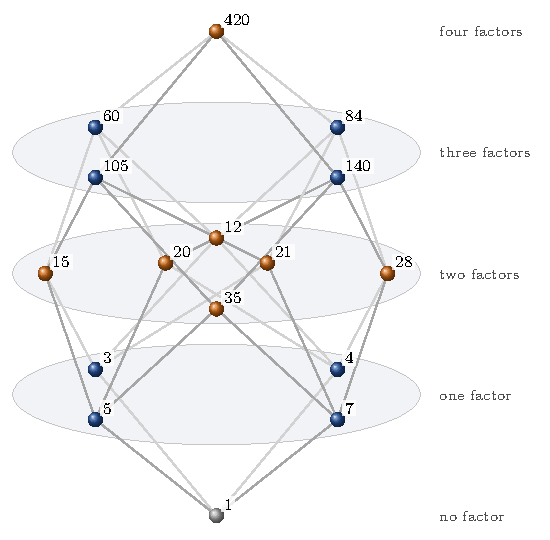
\includegraphics[width=0.72\textwidth]{figures/fig_aoki}
\caption{The products of distinct elements of $\mathsf P$ that divide
$2^{a}3^{b}5^{c}7^{d}$ for large exponents, arranged by the number of
factors, with an edge for each added factor. The products of an even number
of factors, in orange, form $\mathcal Q(M)$; each carries one class
$\xi_{q}$ of \Cref{thm:aoki}.}\label{fig:aoki}
\end{figure}

\begin{theorem}[Aoki]\label{thm:aoki}
For every $q\in\mathcal Q(M)$ there is an element $\xi_{q}\in B_{q}$ such that
\[
  B_{M}=S_{M}+\sum_{q\in\mathcal Q(M)}\ \sum_{t\in(\ZZ/M)^{\times}}
  \ZZ\,t\cdot(M/q)_{*}\xi_{q}.
\]
Moreover $2x\in S_{M}$ and $x+t\cdot x\in S_{M}$ for every $x\in B_{M}$ and
every unit $t$.
\end{theorem}

This is \cite[Theorem~2.1]{Aok00}; the second assertion is part of the proof
of \cite[Corollary~2.3]{Aok00}. It rests on \cite[Theorem~D]{Aok83}, where
the groups are normalized differently; Peterson explains the translation
\cite[\S5.2]{Pet26}.\footnote{Aoki also shows that $B_{M}/S_{M}\cong
(\ZZ/2)^{|\mathcal Q(M)|}$ \cite[Remark~2.4]{Aok00}, so that none of the
classes $\xi_{q}$ can be omitted. For $M=p^{e}$ and $M=2p^{e}$, with $p$ an
odd prime, $\mathcal Q(M)$ is empty, and \Cref{thm:aoki} with
\Cref{lem:transfer} gives the Hodge conjecture for $X^{n}_{M}$ in every
dimension, a theorem of Aoki \cite{Aok87,Aok00}.} We use it through the
following two consequences. Say that a level $M$ is \emph{complete} if every
balanced multiset of an even number of nonzero elements of $\ZZ/M$ is
algebraic. A complete level has the Hodge conjecture for $X^{n}_{M}$ in every
dimension $n$, by the end of the proof of \Cref{lem:transfer}, and every
divisor of a complete level is complete, by \Cref{lem:algtools}(d).

\begin{proposition}\label{prop:complete}
Let $M\ge3$. If every $q\in\mathcal Q(M)$ is a complete level, then $M$ is
a complete level.
\end{proposition}

\begin{proof}
Each $\xi_{q}\in B_{q}$ is an integral combination of classes of balanced
multisets with an even number of elements, which are algebraic as $q$ is
complete. By \Cref{lem:algtools}(c),(d), $t\cdot(M/q)_{*}\xi_{q}$ is then an
integral combination of classes of algebraic balanced multisets at level
$M$. \Cref{thm:aoki} and \Cref{lem:transfer} give the claim.
\end{proof}

\begin{corollary}\label{cor:Bone}
Suppose that $\mathcal Q(M)$ has exactly one element, and let $\nu\colon
R_{M}\to\ZZ/2$ be a homomorphism that vanishes on $S_{M}$. If $\beta$ is a
balanced multiset of an even number of nonzero elements of $\ZZ/M$ with
$\nu([\beta])=1$, then $B_{M}=S_{M}+\ZZ[\beta]$. This applies to
\[
\begin{array}{@{}l@{\qquad}l@{}}
  M=114,\ \nu=\nu_{19},\ \mathcal Q=\{57\}; & M=102,\ \nu=\nu_{17},\
  \mathcal Q=\{51\};\\
  M=44,\ \nu=\nu_{11},\ \mathcal Q=\{44\}; & M=52,\ \nu=\nu_{13},\
  \mathcal Q=\{52\};\\
  M\in\{33,35,39\},\ \nu=\nu_{R},\ \mathcal Q=\{M\}. &
\end{array}
\]
\end{corollary}

\begin{proof}
Let $\mathcal Q(M)=\{q\}$. By \Cref{thm:aoki}, $B_{M}/S_{M}$ is generated by
the images of the elements $t\cdot(M/q)_{*}\xi_{q}$, and $t\cdot x\equiv-x
\equiv x$ modulo $S_{M}$ for every $x\in B_{M}$. So $B_{M}/S_{M}$ is
generated by one element of order at most $2$. As $\nu([\beta])=1$,
$[\beta]\notin S_{M}$; hence $B_{M}/S_{M}$ has order $2$ and is generated by
the image of $[\beta]$. The homomorphisms named vanish on $S_{M}$ by
\Cref{lem:nu,lem:nusqrt}. The elements of $\mathsf P$ that divide
$114=2\cdot3\cdot19$ are $3$ and $19$, those dividing $102=2\cdot3\cdot17$
are $3$ and $17$, since $2\notin\mathsf P$, those dividing $44=4\cdot11$ and
$52=4\cdot13$ are $4,11$ and $4,13$, and those dividing $33$, $35$, $39$ are
their two prime factors; this gives the values of $\mathcal Q$.
\end{proof}

\subsection{Aoki's degrees}
Aoki proves the Hodge conjecture for every abelian variety of Fermat type of
degree $m$ when $m=2^{a}3^{b}5^{c}7^{d}$ with $c=0$ or $d=0$, and when $m$ is
$p^{e}$ or $2p^{e}$ for a prime $p$ \cite[Theorem~0.1]{Aok00}. Among these
abelian varieties are the powers of the Jacobian of the Fermat curve
$X^{1}_{m}$, and the Fermat varieties of degree $m$ are built from that
curve.

\begin{lemma}\label{lem:abelianfermat}
Let $m\ge1$, let $J$ be the Jacobian of $C=X^{1}_{m}$, and suppose that the
Hodge conjecture holds for $J^{N}$ for every $N$. Then it holds for
$X^{n}_{m}$ for every $n$.
\end{lemma}

\begin{proof}
First, the Hodge conjecture holds for $C^{N}$. Fix $o\in C$ and let
$\iota\colon C\to J$ be the Abel--Jacobi map $x\mapsto[x-o]$; then
$\iota^{*}\colon H^{1}(J)\to H^{1}(C)$ is an isomorphism of Hodge
structures. By the K\"unneth formula, $H^{*}(C^{N})$ is the direct sum of
the sub-Hodge structures $H_{T,V}$, indexed by disjoint subsets $T,V$ of
$\{1,\dots,N\}$, that are the tensor products of $H^{1}(C)$ at the factors in
$T$, of $H^{2}(C)=\QQ[o]$ at those in $V$ and of $H^{0}(C)$ at the others. A
Hodge class $h$ of $C^{N}$ is the sum of its components $h_{T,V}$, which are
Hodge classes, and $h_{T,V}=\pr_{T}^{*}g\cup\prod_{i\in V}\pr_{i}^{*}[o]$
for a Hodge class $g$ in the summand $H^{1}(C)^{\otimes T}$ of
$H^{|T|}(C^{T})$. This summand is the image, under the isomorphism
$(\iota^{T})^{*}$, of the summand $H^{1}(J)^{\otimes T}$ of $H^{|T|}(J^{T})$,
so $g=(\iota^{T})^{*}g'$ for a Hodge class $g'$ on $J^{T}$, which is
algebraic. So $g$ and $h_{T,V}$ are algebraic.

Next, write $X^{j}=X^{j}_{m}$. We show by induction on $j$ that the Hodge
conjecture holds for $C^{k}\times X^{j}$ for every $k$; $X^{0}$ is a set of
$m$ points and $X^{1}=C$, so the cases $j\le1$ are the first step. Let
$j\ge2$, and let $\psi\colon Z\to X^{j}$ be the morphism of the inductive
structure with $r=1$ and $s=j-1$, so that $Z$ is the blow-up of $C\times
X^{j-1}$ along $Y\cong X^{0}\times X^{j-2}$. Then $W=C^{k}\times Z$ is the
blow-up of $C^{k+1}\times X^{j-1}$ along $C^{k}\times Y$, a disjoint union
of $m$ copies of $C^{k}\times X^{j-2}$, of codimension two. By the blow-up
formula \cite[Theorem~7.31]{Voi02b}, the map
\[
  H^{i}(C^{k+1}\times X^{j-1})\oplus H^{i-2}(C^{k}\times Y)(-1)\to
  H^{i}(W),
\]
given by the pull-back and by the pull-back to the exceptional divisor
followed by the push-forward, is an isomorphism of Hodge structures. Both
components carry algebraic classes to algebraic classes, so by
\Cref{lem:lift} and induction the Hodge conjecture holds for $W$. The
morphism $\phi=\mathrm{id}\times\psi\colon W\to C^{k}\times X^{j}$ is
surjective between varieties of the same dimension, and
$\phi_{*}\phi^{*}$ is multiplication by its degree. So a Hodge class $h$ of
$C^{k}\times X^{j}$ is $(\deg\phi)^{-1}\phi_{*}\phi^{*}h$, and $\phi^{*}h$
is algebraic. The case $k=0$ is the claim.
\end{proof}

\begin{proposition}\label{prop:aokidegrees}
Every level $m=2^{a}3^{b}5^{c}7^{d}$ with $c=0$ or $d=0$ is complete. In
particular $12$, $15$, $20$, $21$ and $28$ are complete levels.
\end{proposition}

\begin{proof}
The powers of $J$ are abelian varieties of Fermat type of degree $m$, so
\cite[Theorem~0.1]{Aok00} and \Cref{lem:abelianfermat} give the Hodge
conjecture for $X^{n}_{m}$ for every $n$. If $A$ is a balanced multiset of
$n+2$ nonzero elements of $\ZZ/m$, the line $V(\alpha)$ of
\Cref{prop:fermatchars}(ii) consists of Hodge classes of $X^{n}_{m}$, hence
of algebraic classes.
\end{proof}

\section{Classes supported on divisors}\label{sec:classes}

By \Cref{cor:Bone}, at each of the levels $114$, $44$, $52$, $102$, $33$,
$35$ and $39$ a single balanced multiset $\beta$ with $\nu([\beta])=1$
completes the standard multisets. For $33$ and $39$ the multiset $O_{M}$ of
\Cref{sec:odd} serves. For the other five we take $\beta$ to be the join of
two characters of the Fermat threefold, or of one character of the threefold
and one of the curve, and the main step is to show that the corresponding
pieces of $H^{3}$ of the threefold are supported on divisors. This follows
from a finite set of integers, a block pattern, which makes the quotient of
the threefold by the kernel of the character uniruled.

\subsection{Coniveau}
For a smooth projective variety $V$ let $N^{1}H^{k}(V,\QQ)$ be the set of
classes in $H^{k}(V,\QQ)$ that vanish on $V\setminus D$ for some divisor
$D\subseteq V$. It is a subspace, since a union of two divisors is a
divisor, and every proper closed subset of $V$ lies in a divisor.

\begin{lemma}\label{lem:N1}
Let $V$ and $W$ be smooth projective varieties.
\begin{enumerate}[label=\textup{(\alph*)}]
\item Let $f\colon V\to W$ be a surjective morphism with $\dim V=\dim W$.
Then $f^{*}N^{1}H^{k}(W,\QQ)\subseteq N^{1}H^{k}(V,\QQ)$,
$f_{*}N^{1}H^{k}(V,\QQ)\subseteq N^{1}H^{k}(W,\QQ)$, and $f_{*}f^{*}$ is
multiplication by $\deg f$.
\item There is a divisor $D\subseteq W$ such that $N^{1}H^{k}(W,\QQ)=
\iota_{*}H^{k-2}(\tilde D,\QQ)$, where $\iota\colon\tilde D\to W$ is a
resolution of $D$ followed by the inclusion.
\end{enumerate}
\end{lemma}

\begin{proof}
(a) For an open set $U\subseteq W$ the maps $f^{*}$ and $f_{*}$ commute with
restriction to $U$ and to $f^{-1}(U)$; for $f_{*}$ this is the compatibility
of proper push-forward in Borel--Moore homology, which on a smooth variety
is cohomology by Poincar\'e duality, with restriction to open sets
\cite[\S19.1]{Ful98}. If $y$ vanishes on $W\setminus D$, then $f^{*}y$
vanishes on the complement of $f^{-1}(D)$, a proper closed subset as $f$ is
surjective. If $v$ vanishes on $V\setminus E$ for a divisor $E$, then $f(E)$
has dimension less than $\dim W$, so it lies in a divisor $D$, and $f_{*}v$
vanishes on $W\setminus D$ because $f^{-1}(W\setminus D)\subseteq V\setminus
E$. By the projection formula, $f_{*}f^{*}y=f_{*}(f^{*}y\cup1)=y\cup
f_{*}1=(\deg f)\,y$.

(b) The kernels of the restriction maps $H^{k}(W,\QQ)\to H^{k}(W\setminus
D,\QQ)$ grow with $D$, and $H^{k}(W,\QQ)$ is finite-dimensional, so
$N^{1}H^{k}(W,\QQ)$ is one of these kernels. By a theorem of Deligne
\cite[Corollaire~8.2.8]{Del74}, the sequence $H^{k-2}(\tilde D,\QQ)
\xrightarrow{\iota_{*}}H^{k}(W,\QQ)\to H^{k}(W\setminus D,\QQ)$ is
exact.\footnote{The weight filtration on $H^{k}(W\setminus D)$ starts in
weight $k$, and its lowest piece is the image of $H^{k}(W)$; the kernel of
$H^{k}(W)\to H^{k}(W\setminus D)$ is the image of the cohomology with
supports $H^{k}_{D}(W)$, whose quotient of weight $k$ is the Gysin image of
$H^{k-2}(\tilde D)$, and the purity of $H^{k}(W)$ forces the kernel into
that quotient.}
\end{proof}

\begin{lemma}\label{lem:uniruledN1}
If $Y$ is a smooth projective uniruled threefold, then $N^{1}H^{3}(Y,\QQ)=
H^{3}(Y,\QQ)$.
\end{lemma}

\begin{proof}
As $Y$ is uniruled, there are a smooth projective surface $S$ and a dominant
rational map $\PP^{1}\times S\dashrightarrow Y$. Resolving its points of
indeterminacy \cite{Hir64}, we obtain a smooth projective threefold $W$, a
birational morphism $\sigma\colon W\to\PP^{1}\times S$ and a surjective
morphism $\varphi\colon W\to Y$.

First, $N^{1}H^{3}(\PP^{1}\times S)=H^{3}(\PP^{1}\times S)$. By the
K\"unneth formula, $H^{3}(\PP^{1}\times S,\QQ)$ is the sum of
$\pr^{*}H^{3}(S,\QQ)$ and $h\cup\pr^{*}H^{1}(S,\QQ)$, where $\pr$ is the
projection to $S$ and $h$ is the class of $\{p\}\times S$. The second
summand vanishes on $(\PP^{1}\setminus\{p\})\times S$. Let $C\subseteq S$ be
a smooth hyperplane section. By the Lefschetz hyperplane theorem $H_{1}(C,
\QQ)\to H_{1}(S,\QQ)$ is surjective, so by Poincar\'e duality every class of
$H^{3}(S,\QQ)$ is the Gysin image of a class of $H^{1}(C,\QQ)$, and it
vanishes on $S\setminus C$. So the first summand vanishes on $\PP^{1}\times
(S\setminus C)$.

Next, $N^{1}H^{3}(W)=H^{3}(W)$. The morphism $\sigma$ is an isomorphism over
the complement $U$ of a proper closed subset of $\PP^{1}\times S$. For
$w\in H^{3}(W,\QQ)$ the class $\sigma^{*}\sigma_{*}w-w$ vanishes on
$\sigma^{-1}(U)$, and $\sigma^{*}\sigma_{*}w$ lies in $N^{1}$ by the first
step and \Cref{lem:N1}(a); so $w\in N^{1}H^{3}(W,\QQ)$.

Finally, for $y\in H^{3}(Y,\QQ)$ we have $y=(\deg\varphi)^{-1}\varphi_{*}
\varphi^{*}y$, which lies in $N^{1}H^{3}(Y,\QQ)$ by \Cref{lem:N1}(a).
\end{proof}

\begin{lemma}\label{lem:quotientN1}
Let $X$ be a smooth projective threefold, $K$ a finite group acting on $X$,
and $\rho\colon\tilde Y\to X/K$ a resolution that is an isomorphism over the
smooth locus of $X/K$. If $N^{1}H^{3}(\tilde Y,\QQ)=H^{3}(\tilde Y,\QQ)$,
then $H^{3}(X,\QQ)^{K}\subseteq N^{1}H^{3}(X,\QQ)$.
\end{lemma}

\begin{proof}
We may assume that $K$ acts faithfully. Let $q\colon X\to X/K$ be the
quotient map, $X_{0}\subseteq X$ the dense open set of points with trivial
stabilizer, and $Y_{0}=q(X_{0})$. Then $X_{0}=q^{-1}(Y_{0})$, the variety
$Y_{0}$ is smooth, and $q\colon X_{0}\to Y_{0}$ is a finite \'etale Galois
covering with group $K$, so that $q^{*}q_{*}=\sum_{g\in K}g^{*}$ on the
cohomology of $X_{0}$. The rational map $\theta=\rho^{-1}\circ q\colon
X\dashrightarrow\tilde Y$ is a morphism on $X_{0}$. Resolving its
indeterminacy \cite{Hir64} gives a smooth projective threefold $X''$, a
birational morphism $\sigma\colon X''\to X$ that is an isomorphism over
$X_{0}$, and a surjective morphism $\tau\colon X''\to\tilde Y$ with
$\rho\tau=q\sigma$. If $\tau(p)\in\rho^{-1}(Y_{0})$, then $q\sigma(p)\in
Y_{0}$ and so $\sigma(p)\in X_{0}$. Hence $\tau^{-1}(\rho^{-1}(Y_{0}))=
\sigma^{-1}(X_{0})$, and under the isomorphisms $\sigma^{-1}(X_{0})\cong
X_{0}$ and $\rho^{-1}(Y_{0})\cong Y_{0}$ the restriction of $\tau$ is $q$.

Let $x\in H^{3}(X,\QQ)^{K}$ and $w=\sigma^{*}x$. By the compatibility with
restriction used in the proof of \Cref{lem:N1}(a), the restriction of
$\tau^{*}\tau_{*}w$ to $\sigma^{-1}(X_{0})\cong X_{0}$ is
$\sum_{g\in K}g^{*}(x|_{X_{0}})=|K|\,x|_{X_{0}}$. So $\tau^{*}\tau_{*}w-
|K|\,w$ vanishes on the complement of a proper closed subset of $X''$. Since
$\tau_{*}w\in N^{1}H^{3}(\tilde Y,\QQ)$, \Cref{lem:N1}(a) gives
$\tau^{*}\tau_{*}w\in N^{1}H^{3}(X'',\QQ)$, hence $w\in N^{1}H^{3}(X'',\QQ)$,
and $x=\sigma_{*}\sigma^{*}x=\sigma_{*}w$ lies in $N^{1}H^{3}(X,\QQ)$.
\end{proof}

\subsection{Block patterns}
Let $X=X^{3}_{m}\subseteq\PP^{4}$. Its cohomology $H^{3}(X,\QQ)$ is
primitive, and by \Cref{prop:fermatchars}(i), $H^{3}(X,\CC)$ is the direct
sum of the lines $V(a)$, $a\in\mathfrak A^{3}_{m}$, with $V(a)\subseteq
H^{3-q,q}$ for $q=\langle a\rangle-1$. As in the proof of
\Cref{prop:fermatchars}(ii), for $a\in\mathfrak A^{3}_{m}$ the sum
$\bigoplus_{t}V(ta)$ over the units $t$ is defined over $\QQ$; let
$M_{a}\subseteq H^{3}(X,\QQ)$ be the rational sub-Hodge structure with
$M_{a}\otimes\CC=\bigoplus_{t}V(ta)$.

Fix $\alpha\in\mathfrak A^{3}_{m}$, with representatives $\bar\alpha_{k}\in
\{1,\dots,m-1\}$ of its entries, and write $g\cdot\bar\alpha=\sum_{k}g_{k}
\bar\alpha_{k}$ for $g\in\ZZ^{5}$.

\begin{definition}\label{def:blockpattern}
A \emph{block pattern} for $\alpha$ consists of integers $\delta_{1},\dots,
\delta_{r}\ge1$ and $e_{kl}\ge0$ ($0\le k\le4$, $1\le l\le r$) such that
\begin{enumerate}[label=\textup{(P\arabic*)}]
\item $D=\sum_{l}e_{kl}\delta_{l}$ does not depend on $k$;
\item for every $l$, some $e_{kl}$ is positive, some $e_{kl}$ vanishes, and
the column $e_{l}=(e_{0l},\dots,e_{4l})$ has $e_{l}\cdot\bar\alpha\equiv0
\pmod m$;
\item $\sum_{l}\delta_{l}>D$.
\end{enumerate}
\end{definition}

The integers have a geometric meaning: a column $e_{l}$ with degree
$\delta_{l}$ stands for a binary form of degree $\delta_{l}$, and $D$ is the
degree of a rational curve $s\mapsto[u_{0}(s):\dots:u_{4}(s)]$ with
$u_{k}=\prod_{l}P_{l}^{e_{kl}}$ for binary forms $P_{l}$ of degree
$\delta_{l}$. Condition (P2) makes the monomials $\prod_{k}u_{k}^{\bar
\alpha_{k}}$ powers of $m$-th powers, and (P3) says that such curves move in
families large enough to sweep out the quotient below; the proof uses only
the integers.

Let $T=(\CC^{\times})^{5}/\CC^{\times}\subseteq\PP^{4}$ be the open torus.
Its character lattice is $M_{0}=\{u\in\ZZ^{5}:\ \sum_{k}u_{k}=0\}$, the
character $u$ being the function $x^{u}=\prod_{k}x_{k}^{u_{k}}$. The group
$G=\mu_{m}^{5}/\mu_{m}$ is a subgroup of $T$, and $g\in G$ multiplies $x^{u}$
by the value at $g$ of the character $u\bmod m$ of $G$. Let $K=\ker\alpha
\subseteq G$. The characters of $G$ that are trivial on $K$ are the multiples
of $\alpha$, so $T/K$ is a torus with character lattice
\[
  L_{\alpha}=\{u\in M_{0}:\ u\equiv j\bar\alpha\pmod m\ \text{for some}\
  j\in\ZZ\}.
\]
The open set $X^{\circ}=X\cap T$ is stable under $G$, and $X^{\circ}/K$ is
the hypersurface in $T/K$ defined by the $K$-invariant Laurent polynomial
\[
  f=\sum_{k=0}^{4}x^{m(e_{k}-e_{0})}=x_{0}^{-m}\sum_{k=0}^{4}x_{k}^{m},
\]
where $e_{0},\dots,e_{4}$ is the standard basis of $\ZZ^{5}$; it is a dense
open subset of $X/K$. The Newton polytope of $f$ is the simplex
$P\subseteq L_{\alpha}\otimes\RR=M_{0}\otimes\RR$ with the five vertices
$m(e_{k}-e_{0})$, which lie in $L_{\alpha}$. As the coefficients of $f$ at
these vertices do not vanish, $f$ is nondegenerate with respect to $P$
\cite[Example~5.2]{Bat24}. Following Batyrev \cite[Definition~1.2]{Bat24},
the \emph{Fine interior} $F(P)$ is the set of points $y\in P$ with
$\nu(y)-\min_{P}\nu\ge1$ for every nonzero $\nu$ in the dual lattice
$L_{\alpha}^{\vee}=\operatorname{Hom}(L_{\alpha},\ZZ)$.

\begin{lemma}\label{lem:fine}
\begin{enumerate}[label=\textup{(\alph*)}]
\item The nonzero elements of $L_{\alpha}^{\vee}$ are the functionals
$\nu_{g}(u)=(g\cdot u)/m$ with $g\in\ZZ^{5}$ not constant and
$g\cdot\bar\alpha\equiv0\pmod m$. For $y=\sum_{k}y_{k}\,m(e_{k}-e_{0})\in P$,
with $y_{k}\ge0$ and $\sum_{k}y_{k}=1$, one has
$\nu_{g}(y)-\min_{P}\nu_{g}=\sum_{k}y_{k}g_{k}-\min_{k}g_{k}$.
\item If $\alpha$ admits a block pattern, then $F(P)$ is empty.
\end{enumerate}
\end{lemma}

\begin{proof}
(a) A linear form $\nu$ on $M_{0}\otimes\RR$ that is integral on
$L_{\alpha}\supseteq mM_{0}$ has $m\nu$ integral on $M_{0}$, so $m\nu(u)=
g\cdot u$ for some $g\in\ZZ^{5}$, and $\nu\ne0$ exactly when $g$ is not
constant. The vector $u=\bar\alpha-\langle\alpha\rangle me_{0}$ lies in
$L_{\alpha}$, and $g\cdot u\equiv g\cdot\bar\alpha\pmod m$; so
$g\cdot\bar\alpha\equiv0$. Conversely, if $g\cdot\bar\alpha\equiv0$ and
$u\equiv j\bar\alpha\pmod m$, then $g\cdot u\equiv jg\cdot\bar\alpha\equiv0$,
and $\nu_{g}$ is integral on $L_{\alpha}$. Since $\nu_{g}(m(e_{k}-e_{0}))=
g_{k}-g_{0}$, we get $\nu_{g}(y)=\sum_{k}y_{k}g_{k}-g_{0}$, and the minimum
of $\nu_{g}$ on the simplex $P$ is attained at a vertex, so it is
$\min_{k}g_{k}-g_{0}$.

(b) Let $(\delta_{l},e_{kl})$ be a block pattern and $y\in F(P)$, with
barycentric coordinates $y_{k}$ as in (a). By (P2) and (a), each column
$e_{l}$ defines a nonzero $\nu_{e_{l}}\in L_{\alpha}^{\vee}$ with
$\min_{k}e_{kl}=0$, so $\sum_{k}y_{k}e_{kl}\ge1$. Multiplying by $\delta_{l}$,
adding over $l$ and using (P1),
\[
  \sum_{l}\delta_{l}\le\sum_{l}\delta_{l}\sum_{k}y_{k}e_{kl}=\sum_{k}y_{k}
  \sum_{l}e_{kl}\delta_{l}=D\sum_{k}y_{k}=D,
\]
which contradicts (P3).
\end{proof}

\begin{theorem}\label{thm:uniruled}
Let $\alpha\in\mathfrak A^{3}_{m}$ admit a block pattern, and let
$K=\ker\alpha\subseteq G$. Then every smooth projective variety birational to
$X^{3}_{m}/K$ is uniruled, and $M_{\alpha}\subseteq N^{1}H^{3}(X^{3}_{m},
\QQ)$.
\end{theorem}

\begin{proof}
Let $\tilde Y$ be a smooth projective variety birational to $X/K$. By
\Cref{lem:fine}(b) and Batyrev's theorem \cite[Corollary~5.6]{Bat24}, the
nondegenerate hypersurface $X^{\circ}/K$ has negative Kodaira dimension;
since $X^{\circ}/K$ is birational to $\tilde Y$, so has $\tilde Y$. A smooth
projective threefold of negative Kodaira dimension is uniruled: by Mori's
theorem \cite{Mor88} it is birational to a projective threefold $Y'$ with
terminal singularities that is either minimal, with $K_{Y'}$ nef, or the
total space of a Mori fibre space. In the first case $Y'$ would have
nonnegative Kodaira dimension by Miyaoka's theorem \cite{Miy88}. In the
second, a general fibre $F$ has $-K_{F}$ ample, so $K_{F}$ is negative on
the curves cut out on $F$ by general ample divisors, and $F$ is uniruled by
the criterion of Miyaoka and Mori \cite{MM86}; hence $Y'$ is uniruled, and so
is $\tilde Y$.

Choose $\tilde Y$ to be a resolution of $X/K$ that is an isomorphism over
the smooth locus \cite{Hir64}. By \Cref{lem:uniruledN1},
$N^{1}H^{3}(\tilde Y,\QQ)=H^{3}(\tilde Y,\QQ)$, and by
\Cref{lem:quotientN1}, $H^{3}(X,\QQ)^{K}\subseteq N^{1}H^{3}(X,\QQ)$. For a
unit $t$ the character $t\alpha$ is trivial on $K$, so $K$ acts trivially on
$V(t\alpha)$ and on $M_{\alpha}$, and $M_{\alpha}\subseteq H^{3}(X,\QQ)^{K}$.
\end{proof}

\subsection{Joins}
The joins below use the inductive structure of \Cref{sec:fermat}: for
$r,s\ge1$ the map $f\colon H^{r+s-2}(X^{r-1}_{m}\times X^{s-1}_{m})\to
H^{r+s}(X^{r+s}_{m})$ carries $V(a')\otimes V(b')$ onto $V(a'*b')$ and
algebraic classes to algebraic classes.

\begin{proposition}\label{prop:joindivisor}
Let $\alpha,\alpha'\in\mathfrak A^{3}_{m}$ with $M_{\alpha}$ and
$M_{\alpha'}$ contained in $N^{1}H^{3}(X^{3}_{m},\QQ)$.
\begin{enumerate}[label=\textup{(\alph*)}]
\item If $\langle t\alpha\rangle+\langle t\alpha'\rangle=5$ for every unit
$t$, then the multiset of the ten entries of $\alpha$ and $\alpha'$ is
balanced and algebraic.
\item If $b\in\mathfrak A^{1}_{m}$ and $\langle t\alpha\rangle+\langle
tb\rangle=4$ for every unit $t$, then the multiset of the eight entries of
$\alpha$ and $b$ is balanced and algebraic.
\end{enumerate}
\end{proposition}

\begin{proof}
(a) Let $X=X^{3}_{m}$. The multiset is balanced, because for every unit $t$
the representatives of the entries of $t\alpha$ and $t\alpha'$ add up to
$5m$. For every $t$, one of $V(t\alpha)$, $V(t\alpha')$ lies in $H^{2,1}$
and the other in $H^{1,2}$, as $\langle ta\rangle\in\{1,\dots,4\}$ and
$\langle-ta\rangle=5-\langle ta\rangle$ force both values into $\{2,3\}$. So
$L=\bigoplus_{t}V(t\alpha)\otimes V(t\alpha')\subseteq H^{6}(X\times X,\CC)$
has type $(3,3)$. It is stable under $\operatorname{Gal}(\QQ(\mu_{m})/\QQ)$,
so $L=L_{\QQ}\otimes\CC$ for a space $L_{\QQ}\subseteq M_{\alpha}\otimes
M_{\alpha'}$ of Hodge classes.

By \Cref{lem:N1}(b) there are smooth projective surfaces $\tilde D,\tilde D'$
with morphisms $\iota\colon\tilde D\to X$, $\iota'\colon\tilde D'\to X$ such
that $M_{\alpha}\subseteq\iota_{*}H^{1}(\tilde D,\QQ)$ and $M_{\alpha'}
\subseteq\iota'_{*}H^{1}(\tilde D',\QQ)$. The map
\[
  \gamma=(\iota\times\iota')_{*}\colon H^{1}(\tilde D,\QQ)\otimes
  H^{1}(\tilde D',\QQ)(-2)\to H^{3}(X,\QQ)\otimes H^{3}(X,\QQ)
\]
is a morphism of polarizable Hodge structures of weight $6$, given by
$\pm\iota_{*}\otimes\iota'_{*}$ in the K\"unneth decomposition, and its image
contains $M_{\alpha}\otimes M_{\alpha'}$. Applying \Cref{lem:lift} to the
restriction of $\gamma$ to $\gamma^{-1}(M_{\alpha}\otimes M_{\alpha'})$,
every $\upsilon\in L_{\QQ}$ is $\gamma(\upsilon')$ for a Hodge class
$\upsilon'$ in $H^{1}(\tilde D)\otimes H^{1}(\tilde D')(-2)$, that is, a
Hodge class of degree $2$ on $\tilde D\times\tilde D'$. By \Cref{thm:lef11}
it is algebraic, and so is $\upsilon=(\iota\times\iota')_{*}\upsilon'$.
Hence $V(\alpha)\otimes V(\alpha')\subseteq\Alg^{3}(X\times X)\otimes\CC$,
and by the inductive structure with $r=s=4$ the line $V(\alpha*\alpha')=
f\bigl(V(\alpha)\otimes V(\alpha')\bigr)$ is algebraic.

(b) Let $X'=X^{1}_{m}$. The multiset is balanced because the entries of
$t\alpha$ and $tb$ add up to $4m$. As $\langle tb\rangle\in\{1,2\}$, we have
$\langle t\alpha\rangle\in\{2,3\}$, and $V(t\alpha)\subseteq H^{2,1}(X)$
exactly when $V(tb)\subseteq H^{0,1}(X')$; so $\bigoplus_{t}V(t\alpha)
\otimes V(tb)\subseteq H^{4}(X\times X',\CC)$ has type $(2,2)$, and as in (a)
it is $L_{\QQ}\otimes\CC$ for a space $L_{\QQ}\subseteq M_{\alpha}\otimes
H^{1}(X',\QQ)$ of Hodge classes. With $\tilde D$ and $\iota$ as in (a), the
map $(\iota\times\mathrm{id})_{*}\colon H^{1}(\tilde D,\QQ)\otimes
H^{1}(X',\QQ)(-1)\to H^{3}(X,\QQ)\otimes H^{1}(X',\QQ)$ has image containing
$M_{\alpha}\otimes H^{1}(X',\QQ)$, and \Cref{lem:lift} lifts every
$\upsilon\in L_{\QQ}$ to a Hodge class of degree $2$ on the threefold
$\tilde D\times X'$. It is algebraic by \Cref{thm:lef11}, so $\upsilon$ is
algebraic, and the inductive structure with $r=4$ and $s=2$ shows that
$V(\alpha*b)$ is algebraic.
\end{proof}

\subsection{Five pairs of characters}
For a character $a$ of $X^{3}_{m}$ or $X^{1}_{m}$ we have $\langle-ta\rangle
=5-\langle ta\rangle$, respectively $3-\langle ta\rangle$, so it suffices to
list the values at the units $t<m/2$. Each value is the sum of the
representatives in $\{1,\dots,m-1\}$ of the entries of $ta$, divided by $m$.

\begin{lemma}\label{lem:charpairs}
In each line of the following list, the characters named satisfy the
hypothesis of \Cref{prop:joindivisor}(a) or~(b), and the multiset $\beta$ of
their entries is balanced, contains no pair, and has $\nu([\beta])=1$ for the
homomorphism $\nu$ of \Cref{cor:Bone}.
\begin{enumerate}[label=\textup{(\roman*)}]
\item $m=114$: $\alpha_{1}=(1,25,43,57,102)$, $\alpha_{2}=(39,63,68,80,92)$,
$\beta=\{1,\allowbreak 25,\allowbreak 39,\allowbreak 43,\allowbreak 57,\allowbreak 63,\allowbreak 68,\allowbreak 80,\allowbreak 92,\allowbreak 102\}$, $\nu=\nu_{19}$.
\item $m=44$: $\alpha=(1,5,8,33,41)$, $b=(9,37,42)$,
$\beta=\{1,\allowbreak 5,\allowbreak 8,\allowbreak 9,\allowbreak 33,\allowbreak 37,\allowbreak 41,\allowbreak 42\}$, $\nu=\nu_{11}$.
\item $m=52$: $\alpha=(1,5,16,37,45)$, $\alpha'=(29,18,42,50,17)$,
$\beta=\{1,\allowbreak 5,\allowbreak 16,\allowbreak 17,\allowbreak 18,\allowbreak 29,\allowbreak 37,\allowbreak 42,\allowbreak 45,\allowbreak 50\}$, $\nu=\nu_{13}$.
\item $m=102$: $\alpha=(1,7,51,60,85)$, $\alpha'=(91,34,26,98,57)$,
$\beta=\{1,\allowbreak 7,\allowbreak 26,\allowbreak 34,\allowbreak 51,\allowbreak 57,\allowbreak 60,\allowbreak 85,\allowbreak 91,\allowbreak 98\}$, $\nu=\nu_{17}$.
\item $m=35$: $\alpha=(1,2,16,21,30)$, $b=(17,22,31)$,
$\beta=\{1,\allowbreak 2,\allowbreak 16,\allowbreak 17,\allowbreak 21,\allowbreak 22,\allowbreak 30,\allowbreak 31\}$, $\nu=\nu_{R}$.
\end{enumerate}
\end{lemma}

\begin{proof}
The entries are nonzero and the entry sums are multiples of $m$: $228$ and
$342$ in (i), $88$ and $88$ in (ii), $104$ and $156$ in (iii), $204$ and
$306$ in (iv), $70$ and $70$ in (v). The values at the units $t<m/2$ are:

\smallskip
\noindent(i) $m=114$:
\begin{center}
\small
\setlength{\tabcolsep}{3.2pt}
\begin{tabular}{l*{18}{c}}
\toprule
$t$ & 1 & 5 & 7 & 11 & 13 & 17 & 23 & 25 & 29 & 31 & 35 & 37 & 41 & 43 & 47 & 49 & 53 & 55\\
\midrule
$\langle t\alpha_{1}\rangle$ & 2&2&2&2&3&2&2&2&3&3&2&2&3&2&2&3&3&2\\
$\langle t\alpha_{2}\rangle$ & 3&3&3&3&2&3&3&3&2&2&3&3&2&3&3&2&2&3\\
\bottomrule
\end{tabular}
\end{center}
(ii) $m=44$:
\begin{center}
\small
\begin{tabular}{l*{10}{c}}
\toprule
$t$ & 1 & 3 & 5 & 7 & 9 & 13 & 15 & 17 & 19 & 21\\
\midrule
$\langle t\alpha\rangle$ & 2&2&3&2&2&2&3&3&2&3\\
$\langle tb\rangle$ & 2&2&1&2&2&2&1&1&2&1\\
\bottomrule
\end{tabular}
\end{center}
(iii) $m=52$:
\begin{center}
\small
\begin{tabular}{l*{12}{c}}
\toprule
$t$ & 1 & 3 & 5 & 7 & 9 & 11 & 15 & 17 & 19 & 21 & 23 & 25\\
\midrule
$\langle t\alpha\rangle$ & 2&2&2&2&3&2&3&2&3&2&2&3\\
$\langle t\alpha'\rangle$ & 3&3&3&3&2&3&2&3&2&3&3&2\\
\bottomrule
\end{tabular}
\end{center}
(iv) $m=102$:
\begin{center}
\small
\setlength{\tabcolsep}{4pt}
\begin{tabular}{l*{16}{c}}
\toprule
$t$ & 1 & 5 & 7 & 11 & 13 & 19 & 23 & 25 & 29 & 31 & 35 & 37 & 41 & 43 & 47 &
49\\
\midrule
$\langle t\alpha\rangle$ & 2&2&2&2&3&2&2&3&2&2&2&3&2&3&2&3\\
$\langle t\alpha'\rangle$ & 3&3&3&3&2&3&3&2&3&3&3&2&3&2&3&2\\
\bottomrule
\end{tabular}
\end{center}
(v) $m=35$:
\begin{center}
\small
\begin{tabular}{l*{12}{c}}
\toprule
$t$ & 1 & 2 & 3 & 4 & 6 & 8 & 9 & 11 & 12 & 13 & 16 & 17\\
\midrule
$\langle t\alpha\rangle$ & 2&2&2&2&2&3&2&2&2&3&3&3\\
$\langle tb\rangle$ & 2&2&2&2&2&1&2&2&2&1&1&1\\
\bottomrule
\end{tabular}
\end{center}
For instance, in (v), $8\alpha=(8,16,23,28,30)$ and $8b=(31,1,3)$ have
entry sums $105$ and $35$.

In each line the representatives of the entries of $t\beta$ add up to
$m(\langle t\alpha\rangle+\langle t\alpha'\rangle)$ or $m(\langle t\alpha
\rangle+\langle tb\rangle)$, a constant, so $\beta$ is balanced; and no two
entries of $\beta$ add up to $m$. The elements of order $19$ in $\ZZ/114$ are
the nonzero multiples of $6$, and $102$ is the only entry of $\beta$ of this
kind in (i); the elements of order $11$ in $\ZZ/44$ and of order $13$ in
$\ZZ/52$ are the nonzero multiples of $4$, and $8$, respectively $16$, is
the only such entry in (ii), (iii); the elements of order $17$ in $\ZZ/102$
are the nonzero multiples of $6$, and $60$ is the only such entry in (iv).
In (v) the elements of $\ZZ/35$ with square $1$ are $1$, $6$, $29$ and
$34$, and only $1$ is an entry of $\beta$.
\end{proof}

\begin{corollary}\label{cor:patterns}
Each of the characters in the following table admits the block pattern
listed, a column $e_{l}$ with degree $\delta_{l}$ being written
$e_{l}{:}\delta_{l}$:
\begin{center}
\small
\setlength{\tabcolsep}{4pt}
\begin{tabular}{@{}llc>{\raggedright\arraybackslash}p{0.52\textwidth}@{}}
\toprule
$m$ & $\alpha$ & $D$ & block pattern\\
\midrule
$114$ & $13\alpha_{2}=(51,21,86,14,56)$ & $3$ & $(0,0,1,2,0){:}1$,
$(0,0,2,0,1){:}1$, $(1,3,0,0,0){:}1$, $(2,0,0,1,2){:}1$\\
$114$ & $\alpha_{1}=(1,25,43,57,102)$ & $24$ & $(3,1,2,0,0){:}7$,
$(0,1,5,0,1){:}2$, $(0,0,0,2,0){:}12$, $(1,5,0,0,1){:}3$,
$(0,0,0,0,19){:}1$\\
$44$ & $(1,5,8,33,41)$ & $11$ & $(3,0,0,0,1){:}1$, $(0,0,11,0,0){:}1$,
$(1,1,0,0,2){:}5$, $(1,2,0,1,0){:}3$, $(0,0,0,4,0){:}2$\\
$52$ & $(1,5,16,37,45)$ & $14$ & $(0,0,0,3,1){:}4$, $(0,1,1,0,3){:}1$,
$(2,1,0,0,1){:}7$, $(0,0,13,0,0){:}1$, $(0,3,0,1,0){:}2$\\
$52$ & $9\alpha'=(1,6,14,34,49)$ & $5$ & $(0,0,5,1,0){:}1$,
$(3,0,0,0,1){:}1$, $(2,0,0,3,0){:}1$, $(0,3,0,1,0){:}1$,
$(0,1,0,0,2){:}2$\\
$102$ & $37\alpha'=(1,34,44,56,69)$ & $6$ & $(0,0,0,3,2){:}1$,
$(0,0,3,0,4){:}1$, $(0,3,0,0,0){:}2$, $(2,0,1,1,0){:}3$\\
$102$ & $5\alpha=(5,35,51,96,17)$ & $18$ & $(0,0,0,0,6){:}2$,
$(0,0,0,17,0){:}1$, $(0,0,2,0,0){:}9$, $(0,6,0,1,0){:}1$,
$(3,2,0,0,1){:}6$\\
$35$ & $(1,2,16,21,30)$ & $50$ & $(0,0,0,5,0){:}10$, $(1,1,2,0,0){:}25$,
$(1,2,0,0,1){:}10$, $(3,1,0,0,1){:}5$, $(0,0,0,0,35){:}1$\\
\bottomrule
\end{tabular}
\end{center}
In each row the degrees add up to $D+1$. Hence $M_{\alpha}\subseteq N^{1}H^{3}
(X^{3}_{m},\QQ)$ for each of these characters.
\end{corollary}

\begin{proof}
Condition (P1) says that each of the five coordinates of $\sum_{l}\delta_{l}
e_{l}$ equals $D$; for instance, in the second row these coordinates are
$21+3$, $7+2+15$, $14+10$, $24$ and $2+3+19$, and in the last row they are
$25+10+15$, $25+20+5$, $50$, $50$ and $10+5+35$. Condition (P2) is the
divisibility of the weights $e_{l}\cdot\bar\alpha$ by $m$. Row by row, the
weights are
\[
\begin{array}{@{}l@{\qquad}l@{}}
  114,\ 228,\ 114,\ 228; & 114,\ 342,\ 114,\ 228,\ 1938;\\
  44,\ 88,\ 88,\ 44,\ 132; & 156,\ 156,\ 52,\ 208,\ 52;\\
  104,\ 52,\ 104,\ 52,\ 104; & 306,\ 408,\ 102,\ 102;\\
  102,\ 1632,\ 102,\ 306,\ 102; & 105,\ 35,\ 35,\ 35,\ 1050;
\end{array}
\]
for instance $(0,0,1,2,0)\cdot(51,21,86,14,56)=86+28$. The degrees add up to
$4$, $25$, $12$, $15$, $6$, $7$, $19$ and $51$, which is (P3).
\Cref{thm:uniruled} gives the last assertion.
\end{proof}

\begin{theorem}\label{thm:classes}
The levels $33$, $35$, $39$, $44$, $52$, $102$ and $114$ are complete, and so
are $51$ and $57$.
\end{theorem}

\begin{proof}
For $M\in\{33,39\}$, $O_{M}$ is balanced and algebraic by
\Cref{lem:exceptional}. The elements of $\ZZ/33$ with square $1$ are $1$,
$10$, $23$, $32$, and those of $\ZZ/39$ are $1$, $14$, $25$, $38$; of these,
$O_{33}=\{1,4,16,22,25,31\}$ and $O_{39}=\{1,7,16,22,34,37\}$ contain only
$1$. So $\nu_{R}([O_{M}])=1$, and by \Cref{cor:Bone}, $B_{M}=S_{M}+
\ZZ[O_{M}]$.

For the other five levels let $\beta$ be the multiset of \Cref{lem:charpairs}.
Since $M_{ta}=M_{a}$ for every unit $t$, \Cref{cor:patterns} shows that
$M_{\alpha}$, and $M_{\alpha'}$ in (i), (iii), (iv), lie in
$N^{1}H^{3}(X^{3}_{m},\QQ)$: in (i), $M_{\alpha_{2}}=M_{13\alpha_{2}}$; in
(iii), $M_{\alpha'}=M_{9\alpha'}$; in (iv), $M_{\alpha}=M_{5\alpha}$ and
$M_{\alpha'}=M_{37\alpha'}$. By \Cref{prop:joindivisor}, $\beta$ is
algebraic, and by \Cref{cor:Bone}, $B_{m}=S_{m}+\ZZ[\beta]$.

In all seven cases \Cref{lem:transfer} shows that the level is complete.
The levels $57$ and $51$ divide $114$ and $102$.
\end{proof}

\begin{corollary}\label{cor:degrees}
The following levels $M$ are complete, and the Hodge conjecture holds for
$X^{n}_{M}$ for every $n$:
\begin{enumerate}[label=\textup{(\roman*)}]
\item $M=2^{a}3^{b}5^{c}7^{d}$ with $420\nmid M$;
\item $M=2^{a}3^{b}11^{c}$ and $M=2^{a}3^{b}13^{c}$;
\item $M=2^{a}3^{b}17^{c}$ and $M=2^{a}3^{b}19^{c}$ with $a\le1$.
\end{enumerate}
\end{corollary}

\begin{proof}
For $M\le2$, $X^{n}_{M}$ is a linear space or a quadric, and every
balanced multiset at level $2$ is a sum of pairs $\{1,1\}$; let $M\ge3$. In
(i), the elements of $\mathsf P$ dividing $M$ are among $4,3,5,7$, so
$\mathcal Q(M)$ is contained in $\{12,15,20,21,28,35,420\}$, and $420\nmid M$
removes the last; in (ii) it is contained in $\{12,33,44\}$ or $\{12,39,52\}$;
in (iii), where $4\nmid M$, in $\{51\}$ or $\{57\}$. These levels are
complete by \Cref{prop:aokidegrees} and \Cref{thm:classes}, and
\Cref{prop:complete} applies.
\end{proof}

Part (i) for the degrees divisible by $35$ is due to Peterson \cite{Pet26},
who proves the case $M=35$ with the character $\alpha$ of
\Cref{lem:charpairs}(v) by a family of curves on $X^{3}_{35}$ and a residue
computation; the block pattern replaces that computation. Parts (ii) and
(iii) are \cite[Theorem~A]{BBe84hc}, where the coniveau step is also proved
by families of curves.

\section{Even degrees prime to three}\label{sec:even}

In this section and the next, $M$ is even and prime to $3$, and $A$ is a
sextuple at level $M$ that contains no pair, is not split and generates
$\ZZ/M$. We look for a chain of moves that succeeds, as required by
\Cref{prop:induction}. The definitions of \Cref{sec:odd} (maximal orders, the
embedding $\kappa$, the function $F$, moves $(\ell,x)$ for $A$) and
\Cref{lem:movecrit,lem:charrel,lem:fiberline} do not use that $M$ is odd, and
we use them as they stand.

The \emph{odd part} of a positive integer $f$ is $f/2^{v_{2}(f)}$. Let
$e^{*}$ be an odd part of an order of an element of $A$ that is maximal for
divisibility among these odd parts, and let $2^{J}e^{*}$ be the largest order
of an element of $A$ with odd part $e^{*}$. Then $2^{J}e^{*}$ is a maximal
order: an order that is a proper multiple of it would have an odd part
divisible by $e^{*}$, hence equal to $e^{*}$, and a larger power of $2$. This
section treats $J=1$, and \Cref{sec:four} treats $J\ge2$.

\subsection{Every maximal order is even}

\begin{lemma}\label{lem:maxeven}
If $A$ has no move, then every maximal order of $A$ is even. In particular
$J\ge1$.
\end{lemma}

\begin{proof}
Let $e$ be an odd maximal order. Since $3\nmid M$, $e$ is prime to $6$, and
$e>1$. As in \Cref{sec:odd}, $F$ is odd, $\|F\|=2N_{e}\le12$, $F(z_{0})\ge1$
when $\kappa(z_{0})\in A$ has order $e$, and $F$ is split along
$(K_{p})_{p\mid e}$ on every coset of $H$, so \Cref{prop:core} applies. In its
case (1), $F\ge1$ on a line $wK_{p}$ with $p\in\{5,7\}$; as $F$ is odd,
$-1\notin K_{p}$, so $e\ne p$, and $|K_{p}|\ge4\ge(p+1)/2$, so $A$ has a move
by \Cref{lem:fiberline}. In case (2), $\|F\|=12$, so the six elements of $A$
have order $35$ and lie in the subgroup of order $35$; they do not generate
$\ZZ/M$, as $M$ is even.
\end{proof}

\subsection{The top order}\label{ssec:top}
From now on in this section $J=1$, and we put $e=2e^{*}$. If $e^{*}=1$, every
odd part is $1$, the largest order is $2$, and $A$ consists of six copies of
$M/2$, which contains a pair; so $e^{*}>1$, and $e^{*}$ is prime to $6$. Let
$U^{*}=(\ZZ/e^{*})^{\times}$. For $v\in U^{*}$ let
\[
  x_{v}=\tfrac{M}{e}\,u\quad(u\ \text{odd},\ u\equiv v\bmod e^{*}),\qquad
  y_{v}=x_{v}+\tfrac M2=\tfrac{M}{e^{*}}\cdot\tfrac{v}{2},
\]
where $v/2$ is taken modulo $e^{*}$. The $x_{v}$ are the elements of order $e$
and the $y_{v}$ those of order $e^{*}$, and
\[
  -x_{v}=x_{-v},\quad -y_{v}=y_{-v},\quad 2x_{v}=y_{2v},\quad
  -2x_{v}=y_{-2v},\quad T(x_{v})=\{x_{v},\,y_{v},\,y_{-2v},\,M/2\}.
\]
Reduction modulo $e^{*}$ identifies $U=(\ZZ/e)^{\times}$ with $U^{*}$, and
$\kappa(u)=x_{u\bmod e^{*}}$. So the function $F$ of \Cref{sec:odd} becomes
$F(v)=\mult_{A}(x_{v})-\mult_{A}(x_{-v})$, and for $p\mid e^{*}$ the subgroup
$K_{p}$ becomes the group of units congruent to $1$ modulo $e^{*}/p$; we
write $H^{*}$ for the product of these subgroups, which is direct
(\Cref{lem:Kp}). Put
\[
  E(v)=\mult_{A}(y_{v})-\mult_{A}(y_{-v}).
\]
Both $F$ and $E$ are odd, and since $A$ contains no pair,
$|F(v)|=\mult_{A}(x_{v})+\mult_{A}(x_{-v})$ and likewise for $E$; so
$\|F\|=2N_{e}$ and $\|E\|=2N_{e^{*}}$, where $N_{f}$ is the number of
elements of $A$ of order $f$. The elements of $A$ of order $e$ are the
\emph{tops}; we say that $v$ is a top if $x_{v}\in A$, that is, if
$F(v)\ge1$. The elements of order other than $e$ and $e^{*}$ are \emph{low},
and there are $6-N_{e}-N_{e^{*}}$ of them.

\begin{lemma}\label{lem:topfibres}
Let $q\mid e^{*}$ be prime and $v\in U^{*}$. The elements $x_{w}$, $w\in
vK_{q}$, lie in $\Phi_{q}(x_{v})$, and so do the elements $y_{w}$, $w\in
vK_{q}$, if $e^{*}\ne q$. If $A$ contains $(q+1)/2$ distinct elements of one
of these two kinds, then $A$ has a move.
\end{lemma}

\begin{proof}
For $w\in vK_{q}$ we have $w\equiv v$ modulo $e^{*}/q$. The representatives
$u,u'$ of $v,w$ in the definition of $x$ can be chosen odd and congruent
modulo $2e^{*}/q$, so $x_{w}-x_{v}\in(M/e)(e/q)\ZZ=(M/q)\ZZ$; likewise
$y_{w}-y_{v}=(M/e^{*})(w-v)/2\in(M/q)\ZZ$. The last assertion is
\Cref{lem:movecrit}, applied with $\ell=q$, which differs from the orders $e$
and $e^{*}$ of these elements.
\end{proof}

\begin{lemma}\label{lem:E1}
Let $E_{1}(w)=E(w)-F(w)+F(w/2)$. Then $E_{1}$ is odd and split along
$(K_{p})_{p\mid e^{*}}$ on every coset of $H^{*}$ in $U^{*}$. It is the
function $w\mapsto\mult_{A_{1}}(y_{w})-\mult_{A_{1}}(y_{-w})$ of the multiset
\[
  A_{1}=A-\sum_{v\ \text{top}}\{x_{v}\}+\sum_{v\ \text{top}}\{y_{-v},\,y_{2v},
  \,M/2\},
\]
the sums running over the tops with their multiplicities, and $A_{1}$ is
the result of the chain of moves $(T(x_{v}),\{x_{v}\})$ over the tops.
\end{lemma}

\begin{proof}
Let $\chi$ be an odd primitive character modulo $e^{*}$. The elements $a$ of
$A$ whose order is divisible by $e^{*}$ have odd part $e^{*}$, by maximality,
so they are the $x_{v}$ and $y_{v}$ in $A$. For $y_{v}$ we have
$z_{a}=v/2$, and for $x_{v}$ we have $z_{a}\equiv v$ modulo $e^{*}$ and the
factor $1-\chi(2)$; and $\varphi(e)=\varphi(e^{*})$. Since $\chi$ is odd,
$\sum_{v}\mult_{A}(y_{v})\bar\chi(v)=\tfrac12\hat E(\chi)$ with $\hat
f(\chi)=\sum_{v}f(v)\bar\chi(v)$, and likewise for $F$. So \eqref{eq:charrel}
reads $\chi(2)\hat E(\chi)+(1-\chi(2))\hat F(\chi)=0$, that is, $\hat
E(\chi)=(1-\bar\chi(2))\hat F(\chi)$. As $\widehat{F(\cdot/2)}(\chi)=
\bar\chi(2)\hat F(\chi)$, we get $\hat E_{1}(\chi)=0$. For even $\chi$,
$\hat E_{1}(\chi)=0$ because $E_{1}$ is odd. So $\hat E_{1}$ vanishes at
every primitive character, and the proof of \Cref{lem:splitF}, with
\Cref{lem:Kp}(c) for $e^{*}$, shows that $E_{1}$ is split on every coset of
$H^{*}$.

The move $(T(x_{v}),\{x_{v}\})$ removes $x_{v}$ and adds
$-y_{v}=y_{-v}$, $-y_{-2v}=y_{2v}$ and $-M/2=M/2$. The function of
$A_{1}$ at $w$ receives $E(w)$ from $A$, $+1$ for each top $v=-w$ and $-1$ for
each top $v=w$, which is $-F(w)$, and $+1$ for each top $v=w/2$ and $-1$ for
each top $v=-w/2$, which is $F(w/2)$.
\end{proof}

\subsection{Elementary moves}

\begin{lemma}\label{lem:elementary}
Let $v$ be a top and $x=x_{v}$. Each of the following is a move that
lowers the profile, or leaves at most four elements after the removal of
pairs.
\begin{enumerate}[label=\textup{(\alph*)}]
\item $y_{v}=x+M/2\in A$: with $S=\{x,x+M/2\}\subseteq T(x)$,
$A''=A-x-(x+M/2)+\{2x,\,M/2\}$.
\item $y_{-2v}=-2x\in A$: with $S=\{x,-2x\}\subseteq T(x)$,
$A''=A-x-(-2x)+\{y_{-v},\,M/2\}$.
\item $2v$ is also a top: with $\sigma=T(x_{2v})+T(x_{v})$ and
$S=\{x_{2v},x_{v}\}$, $A''=A-x_{2v}-x_{v}+\{y_{4v},\,y_{-v}\}$.
\item $M/2\in A$: with $S=\{x,M/2\}\subseteq T(x)$,
$A''=A-x-M/2+\{y_{-v},\,y_{2v}\}$.
\end{enumerate}
\end{lemma}

\begin{proof}
These are instances of \Cref{def:move}. In (c), $\sigma$ is algebraic by
\Cref{lem:algtools}(b),(e), $\sigma-S=\{y_{2v},y_{-4v},M/2,y_{v},y_{-2v},
M/2\}$, and $-(\sigma-S)=\{y_{-2v},y_{4v},M/2,y_{-v},y_{2v},M/2\}$; after
removing the pairs $\{y_{2v},y_{-2v}\}$ and $\{M/2,M/2\}$ the stated multiset
remains. In each case one element of order
$e$ is removed and only elements of order $e^{*}$ or $2$ are added, while the
elements of order larger than $e$ stay. So if six elements remain they form a
sextuple of smaller profile.
\end{proof}

From now on we assume that $A$ has none of the moves of
\Cref{lem:elementary,lem:topfibres}.

\begin{lemma}\label{lem:signs}
For every $w\in U^{*}$ the numbers $E(w)$, $-F(w)$ and $F(w/2)$ do not have
opposite signs, so
\[
  |E_{1}(w)|=|E(w)|+|F(w)|+|F(w/2)|.
\]
Consequently:
\begin{enumerate}[label=\textup{(\roman*)}]
\item $\|E_{1}\|=2N_{e^{*}}+4N_{e}\le24$;
\item at every top $v$, $E_{1}(v)\le-1$ and $E_{1}(2v)\ge1$, so $E_{1}\ne0$;
\item the elements of order $e^{*}$ of $A_{1}$ contain no pair, and
$\mult_{A_{1}}(y_{w})$ is the positive part of $E_{1}(w)$;
\item the negative part of $E_{1}$ is the counting function of the multiset
$\{w:\ y_{-w}\in A\}+\{\text{tops}\}+\{-2v:\ v\ \text{top}\}$.
\end{enumerate}
\end{lemma}

\begin{proof}
If $E(w)\ge1$ and $F(w)\ge1$, then $y_{w}=x_{w}+M/2$ and $x_{w}$ lie in
$A$, which is \Cref{lem:elementary}(a); the same with $-w$ if both are
negative. If $F(w)\le-1$ and $F(w/2)\le-1$, then $-w$ and $-w/2$ are tops,
which is (c); the same with $w$ if $F(w)\ge1$ and $F(w/2)\ge1$. If
$E(w)\ge1$ and $F(w/2)\le-1$, then $y_{w}$ and $x_{-w/2}$ lie in $A$, and
$y_{w}=-2x_{-w/2}$, which is (b); the same with $-w$ in the other case. So
the three numbers never have opposite signs, and the displayed identity
follows. Summing it gives (i), with $N_{e}+N_{e^{*}}\le6$. At a top $v$,
$-F(v)\le-1$ and $F(2v/2)\ge1$, which gives (ii), and $N_{e}\ge1$ since $e$
is an order of $A$. The multiplicity of $y_{w}$ in $A_{1}$ is the sum of the
positive parts of the three numbers, and that of $y_{-w}$ the sum of their
negative parts; so one of them vanishes, which is (iii), and (iv) is the
same computation for the negative parts.
\end{proof}

\subsection{The compound move}
A \emph{non-cancelling line sum} is a function $f=\sum_{i}s_{i}\mathbf
1_{L_{i}}$, for a finite family of lines $L_{i}$ (repetitions allowed) and
signs $s_{i}\in\{\pm1\}$, such that $|f|=\sum_{i}\mathbf 1_{L_{i}}$.

\begin{lemma}\label{lem:linesum}
If $E_{1}$ is a non-cancelling line sum of lines along the subgroups $K_{p}$,
$p\mid e^{*}$, and $e^{*}$ is not prime, then $A$ has a chain of moves that
is direct or lowering.
\end{lemma}

\begin{proof}
Pass from $A$ to $A_{1}$ (\Cref{lem:E1}). By \Cref{lem:signs}(iii), the
elements of order $e^{*}$ of $A_{1}$ are the $y_{w}$ for $w$ in the lines
$L_{i}$ with $s_{i}=1$, each counted once per line. Let $L=wK_{p}$ be such a
line and $y=y_{w}$. By \Cref{lem:topfibres} the $y_{w'}$, $w'\in L$, are
$|K_{p}|$ distinct elements of order $e^{*}$ of the fibre $\Phi_{p}(y)$. If
$p^{2}\mid e^{*}$, they are the whole fibre; if $p\parallel e^{*}$, the fibre
consists of them and one element $y_{0}$ of order $e^{*}/p$. Since $e^{*}$ is
not prime, $py\ne0$, and the move $(\sigma_{p,y},S)$ with $S=\{y_{w'}:w'\in
L\}$ removes these elements and adds $py$, and $-y_{0}$ if $p\parallel e^{*}$:
at most two elements of order dividing $e^{*}/p$. We do this for each positive
line in turn.

Each line has $|K_{p}|\ge4$ points, and the positive lines carry
$\|E_{1}\|/2=N_{e^{*}}+2N_{e}$ points in all, so there are at most
$(N_{e^{*}}+2N_{e})/4$ of them. The multiset $A_{1}$ contains $N_{e}$ copies
of $M/2$, which is not in $A$ by \Cref{lem:elementary}(d); after removing pairs,
$\epsilon\in\{0,1\}$ copies remain, with $\epsilon\equiv N_{e}$ modulo $2$.
The final multiset therefore has at most
\[
  (6-N_{e}-N_{e^{*}})+\epsilon+2\cdot\frac{N_{e^{*}}+2N_{e}}{4}
  =6+\epsilon-\frac{N_{e^{*}}}{2}\le7
\]
elements. It is balanced (\Cref{lem:move}), so its size is even and at most
$6$. It contains the low elements of $A$, at most one copy of $M/2$ and
elements of order smaller than $e^{*}$; so it has no element of order $e$,
the same elements of order larger than $e$ as $A$, and the chain is direct or
lowering.
\end{proof}

\subsection{Split functions of mass at most eight}

\begin{lemma}\label{lem:S}
Let $K_{1},\dots,K_{r}$ be subgroups of a finite abelian group whose product
$H$ is direct, with pairwise distinct orders $|K_{i}|\ge4$, such that the
orders $4$ and $5$ do not both occur. Let $C$ be a coset of $H$ and $f\colon
C\to\ZZ$ split along $(K_{1},\dots,K_{r})$, not identically zero, with
$\sum_{C}|f|\le8$. Then $f$ is one of
\begin{enumerate}[label=\textup{(\roman*)}]
\item $\sigma\mathbf 1_{L}$, with $\sigma=\pm1$ and $L$ a line along some
$K_{i}$;
\item $2\sigma\mathbf 1_{L}$, with $L$ a line along the $K_{i}$ of order $4$;
\item $\sigma\mathbf 1_{L}+\sigma'\mathbf 1_{L'}$, with $L\ne L'$ lines along
the $K_{i}$ of order $4$;
\item a \emph{cross} $\sigma(\mathbf 1_{L}-\mathbf 1_{L'})$, with $L$ a line
along the $K_{i}$ of order $6$, $L'$ a line along the $K_{j}$ of order $4$, and
$|L\cap L'|=1$.
\end{enumerate}
In particular $\sum_{C}|f|\ge\min_{i}|K_{i}|$.
\end{lemma}

\begin{proof}
By induction on $r$; for $r=0$ there is nothing to prove. For $r=1$, $f$ is
constant on the line $C$ by (S4), with a value $c\ne0$ and $|c|\,|K_{1}|\le8$;
so $|c|=1$, case (i), or $|c|=2$ and $|K_{1}|=4$, case (ii). Let $r\ge2$, and
number the subgroups so that $K=K_{1}$ has the largest order; then $|K|\ge5$
and $|K|>m'=\min_{i\ge2}|K_{i}|\ge4$. We use the slices $S_{c}$, $c\in K$, of
\Cref{sec:primetosix}.

\emph{Case A: $f$ is $K$-invariant.} Then $f$ is constant on the lines along
$K$, a nonzero value $c$ gives $|c|\,|K|\le8$, so $|c|=1$, and a second
line on which $f\ne0$ would add $|K|\ge5$ to the mass. This is (i).

\emph{Case B1: $\mu(c_{0})=0$ for some $c_{0}$.} By (S2), $f$ is split along
$(K_{2},\dots,K_{r})$ on every slice. By induction a nonzero slice carries
mass at least $m'\ge4$, so at most two slices are nonzero. If one is, $f$ is
one of (i)--(iv) inside it. If two are, each carries mass $4$ and is of the
form $\sigma\mathbf 1_{L}$ with $|L|=4$; this is (iii).

\emph{Case B2: $f$ is not $K$-invariant and $\mu\ge1$ on every slice.} As
$\sum_{c}\mu(c)\le8<2|K|$, some $c_{s}$ has $\mu(c_{s})=1$. For $c\in K$ the
function $g_{c}(z)=f(z)-f(zc^{-1}c_{s})$ on $S_{c}$ is split along
$(K_{2},\dots,K_{r})$ by (S1), with mass at most $\mu(c)+1\le8$. If every
$g_{c}$ vanished, $f$ would be $K$-invariant. Let $D$ be the set of $c$ with
$g_{c}\ne0$, and $d=|D|\ge1$. For $c\in D$ the induction gives $\mu(c)+1\ge
m'$. Hence
\[
  8\ge\sum_{c}\mu(c)\ge d(m'-1)+(|K|-d),\qquad\text{so}\qquad |K|+d(m'-2)\le8.
\]
With $|K|\ge m'+1$ and $d\ge1$ this forces $m'=4$, $d=1$ and $|K|\le6$; the
value $|K|=5$ is excluded, as the orders $4$ and $5$ do not both occur. So
$|K|=6$, all the inequalities are equalities, $\mu(c_{1})=3$ for the element
$c_{1}$ of $D$, and $\mu=1$ on the other five slices. Off $S_{c_{1}}$, $f$ is
the translate of its restriction to $S_{c_{s}}$, so it equals $\sigma$ at one
point of each slice, and these points lie on one line $L$ along $K$. On
$S_{c_{1}}$, $g_{c_{1}}$ has mass $4$, so by induction it is $\tau\mathbf
1_{L'}$ for a line $L'$ along the subgroup of order $4$; then $f=\sigma\delta_{z_{1}}
+\tau\mathbf 1_{L'}$ on $S_{c_{1}}$, where $z_{1}$ is the point of $L$ in
$S_{c_{1}}$, and the mass $3$ forces $z_{1}\in L'$ and $\tau=-\sigma$. This
is (iv). The last assertion holds in each case.
\end{proof}

For $e^{*}$ prime to $6$ the subgroups $K_{p}$, $p\mid e^{*}$, satisfy the
hypotheses of \Cref{lem:S}: by \Cref{lem:Kp}(a), $|K_{p}|$ is $p-1$ or $p$,
these pairs of integers are disjoint for different primes $p\ge5$, and the
order $4$ occurs only for $5\parallel e^{*}$, the order $5$ only for
$25\mid e^{*}$. A cross needs $5\parallel e^{*}$ and $7\parallel e^{*}$. The
functions (i)--(iii) are non-cancelling line sums, and a cross is not.

\subsection{The cases}
We now show that $E_{1}$ is a non-cancelling line sum, except when $e^{*}$ is
$35$ or $55$, which we treat afterwards.

\begin{lemma}\label{lem:eprime}
$e^{*}$ is not prime.
\end{lemma}

\begin{proof}
If $e^{*}=p$, then $K_{p}=U^{*}=H^{*}$, and $E_{1}$ is constant by (S4) and
odd, so $E_{1}=0$, against \Cref{lem:signs}(ii).
\end{proof}

\begin{proposition}\label{prop:nonsquarefree}
If $e^{*}$ is not squarefree, then $E_{1}$ is a non-cancelling line sum.
\end{proposition}

\begin{proof}
Let $R=\prod_{p^{2}\mid e^{*}}p^{v_{p}(e^{*})-1}$; then $R\ge5$, since
$e^{*}$ is prime to $6$. Every $K_{p}$ consists of units congruent to $1$
modulo $R$, as $R\mid e^{*}/p$, and the group of such units has order
$\prod_{p\parallel e^{*}}(p-1)\prod_{p^{2}\mid e^{*}}p=|H^{*}|$; so $H^{*}$ is
the group of units congruent to $1$ modulo $R$. Hence $-1,2,-2,4\notin H^{*}$,
since $R$ divides none of $2,1,3,3$, and $-4\in H^{*}$ only if $R=5$.

Let $v$ be a top. The cosets $X_{1}=vH^{*}$, $X_{2}=-vH^{*}$, $X_{3}=2vH^{*}$,
$X_{4}=-2vH^{*}$ are distinct, and $E_{1}\ne0$ on each of them by
\Cref{lem:signs}(ii), so each carries mass at least $4$ (\Cref{lem:S}). By
oddness $\mu(X_{1})=\mu(X_{2})=a$ and $\mu(X_{3})=\mu(X_{4})=b$, and
$2a+2b\le24$; so $a,b\le8$, and every other coset, which has the same mass as
its negative, carries at most $4$. So on every coset $E_{1}$ is zero or one of
the functions of \Cref{lem:S}. If no coset carries a cross, $E_{1}$ is a
non-cancelling line sum.

Suppose a coset carries a cross. Then $5\parallel e^{*}$ and $7\parallel
e^{*}$, so the primes of $R$ are at least $11$, $R\ne5$ and $-4\notin H^{*}$.
The coset has mass $8$, so it is one of the $X_{i}$, and $\{a,b\}=\{4,8\}$.
Then $\|E_{1}\|=24=2N_{e^{*}}+4N_{e}$, so $N_{e}=6$, $N_{e^{*}}=0$, and $E_{1}$
vanishes off the $X_{i}$. By \Cref{lem:signs}(iv) the negative part of
$E_{1}$ counts the multiset $T+(-2T)$, $T$ the six tops. A top $t\in
X_{3}\cup X_{4}$ would have $E_{1}(2t)\ne0$ with $2t\in\pm4vH^{*}$, and this
coset is none of the $X_{i}$, as $\pm4,\pm2\notin H^{*}$, $\mp4\notin H^{*}$.
So $T\subseteq X_{1}\cup X_{2}$ and $-2T\subseteq X_{3}\cup X_{4}$, and the
negative mass of $E_{1}$ on $X_{1}\cup X_{2}$ is $|T|=6$. By oddness it is
the total mass $a$ of $E_{1}$ on $X_{1}$, which is $4$ or $8$; a
contradiction.
\end{proof}

\begin{proposition}\label{prop:threeprimes}
If $e^{*}$ is squarefree with at least three prime factors, then $E_{1}$ is
a non-cancelling line sum.
\end{proposition}

\begin{proof}
Here $H^{*}=U^{*}$. Let $p_{1}$ be the largest prime factor, so $p_{1}\ge11$,
and $K=K_{p_{1}}$, of order $p_{1}-1\ge10$. In the coordinates
$U^{*}=(\ZZ/p_{1})^{\times}\times(\ZZ/(e^{*}/p_{1}))^{\times}$ the group $K$ is
the first factor, the product $H'$ of the other $K_{p}$ is the second, and
the slices are $S_{c}=\{c\}\times(\ZZ/(e^{*}/p_{1}))^{\times}$. Write
$-1=\varepsilon\varepsilon'$ with $\varepsilon=(-1,1)\in K$ and
$\varepsilon'=(1,-1)\in H'$. Then $\mu(-c)=\mu(c)$, and for $z\in S_{c}$,
$E_{1}(z\varepsilon)=E_{1}(-z\varepsilon')=-E_{1}(z\varepsilon')$; so by
(S1) the function
\[
  g(z)=E_{1}(z)+E_{1}(z\varepsilon')=E_{1}(z)-E_{1}(z\varepsilon)
  \tag{$*$}
\]
is split along $(K_{p})_{p\ne p_{1}}$ on $S_{c}$, with mass at most
$2\mu(c)$, and $g(z\varepsilon')=g(z)$. The element $\varepsilon'$ lies in no
$K_{p}$ with $p\ne p_{1}$, since it is congruent to $-1$ modulo a third prime
factor. A top in $S_{c}$ makes the slices $S_{c},S_{-c},S_{2c},S_{-2c}$
nonzero (\Cref{lem:signs}(ii)), and they are distinct, as $p_{1}\ge11$.

\emph{Case Z: some slice vanishes.} By (S2), $E_{1}$ is split along
$(K_{p})_{p\ne p_{1}}$ on every slice, so nonzero slices carry mass at least
$4$ (\Cref{lem:S}). For a top in $S_{c}$, the four slices above carry
$2\mu(c)+2\mu(2c)\le24$, so $\mu(c),\mu(2c)\le8$ and every other slice
carries at most $4$. So \Cref{lem:S} applies on every slice, and without a
cross $E_{1}$ is a non-cancelling line sum. A cross has mass $8$, so for each
top it lies on one of the four slices of that top; then $\|E_{1}\|=24$,
$N_{e}=6$, $N_{e^{*}}=0$, and $E_{1}$ vanishes off these four slices, with
$\{\mu(c),\mu(2c)\}=\{4,8\}$. A top $t$ in $S_{\pm2c}$ would have $2t$ in
$S_{\pm4c}$, which is none of the four slices, as $4\not\equiv\pm1,\pm2$
modulo $p_{1}$; but $E_{1}(2t)\ne0$. So the six tops lie in $S_{c}\cup
S_{-c}$, where the negative mass of $E_{1}$ is then $6$ by
\Cref{lem:signs}(iv), while by oddness it is $\mu(c)\in\{4,8\}$.

\emph{Case NZ1: some $\mu(c)=1$.} In $(*)$, $g$ has mass at most $2<4$, so
$g=0$; then $E_{1}(z_{0}\varepsilon')=-E_{1}(z_{0})\ne0$ at the support point
$z_{0}$ of $S_{c}$, and $z_{0}\varepsilon'\ne z_{0}$ is a second point of
$S_{c}$ where $E_{1}\ne0$. A contradiction.

\emph{Case NZ2: all $\mu(c)\ge2$.} Then $2(p_{1}-1)\le24$, so $p_{1}$ is $11$
or $13$. On a slice of mass $2$, $g$ has mass at most $4$; if it is not
zero, it is $\pm\mathbf 1_{L}$ for a line $L$ along $K_{5}$ (\Cref{lem:S}),
and $g(z\varepsilon')=g(z)$ gives $L\varepsilon'=L$, so $\varepsilon'\in
K_{5}$, which we excluded. So on every slice of mass $2$,
$E_{1}=\sigma(\delta_{z_{0}}-\delta_{z_{0}\varepsilon'})$. Two slices
$S_{c},S_{c'}$ of mass $2$ are translates of each other: the function
$h(z)=E_{1}(z)-E_{1}(zc^{-1}c')$ on $S_{c}$ is split along $(K_{p})_{p\ne
p_{1}}$ by (S1), has mass at most $4$ and satisfies
$h(z\varepsilon')=-h(z)$, while a nonzero split function of mass at most $4$
is $\pm\mathbf 1_{L}$, which is not of this kind.

If $p_{1}=13$, the twelve slices all have mass $2$, so $E_{1}$ is
$K$-invariant, and $E_{1}=\sigma(\mathbf 1_{L}-\mathbf 1_{L\varepsilon'})$ for
a line $L$ along $K$, with $L\ne L\varepsilon'$: a non-cancelling line sum.

If $p_{1}=11$, then $e^{*}=385$ and $H'=K_{5}\times K_{7}$, of orders $4$
and $6$. The ten slices carry mass at most $24$, at least $2$ each, and
masses at least $3$ on the others; so at least six slices have mass $2$, and
the others come in pairs $\pm c$ with $\mu(c)\le4$. For such a $c$, the
difference of $E_{1}$ on $S_{c}$ with the translate of a slice of mass $2$ is
split, nonzero and of mass at most $\mu(c)+2\le6$, so by \Cref{lem:grid} it
is $\pm\mathbf 1_{L'}$ for a line $L'$ along $K_{5}$ or $K_{7}$. The line
$L'$ contains at most one of the two support points
$z_{0},z_{0}\varepsilon'$ of the translate, as $\varepsilon'$ lies in neither
$K_{5}$ nor $K_{7}$; so $\mu(c)\ge|L'|\ge4$. Hence $\mu(c)=4$, $L'$ is a line along
$K_{5}$ through one of the two points, exactly two slices $S_{\pm c_{1}}$ have
mass $4$, the total is $24$, and $N_{e}=6$. In coordinates $(a,b)\in
(\ZZ/11)^{\times}\times(\ZZ/35)^{\times}$ the support of $E_{1}$ lies in
$\{b=\pm b_{0}\}\cup\{a=\pm c_{1},\ b\in\pm b_{0}K_{5}\}$, where $K_{5}$ is
the group of units congruent to $1$ modulo $7$. For $t=(a,b)$ in this set,
$2t$ lies outside it: $2\not\equiv\pm1$ modulo $35$ and modulo $11$, and
$\pm2,\pm\frac12\notin K_{5}$. By \Cref{lem:signs}(ii) there is then no
top, against $N_{e}=6$.
\end{proof}

\begin{proposition}\label{prop:twoprimes}
Let $e^{*}=pq$ with primes $5\le p<q$. Write $E_{1}(y,x)$ for
$(y,x)\in(\ZZ/p)^{\times}\times(\ZZ/q)^{\times}=U^{*}$. Then
$E_{1}(y,x)=\alpha(x)+\beta(y)$ with odd functions $\alpha,\beta$, either both
with values in $\ZZ$ or both with values in $\frac12+\ZZ$, and
\[
  \|E_{1}\|=\sum_{y,x}\max\bigl(|\alpha(x)|,|\beta(y)|\bigr).
\]
If $e^{*}\notin\{35,55\}$, or if $\alpha$ or $\beta$ is zero, then $E_{1}$ is
a non-cancelling line sum.
\end{proposition}

\begin{proof}
Here $H^{*}=U^{*}$, $K_{p}=(\ZZ/p)^{\times}\times\{1\}$ and
$K_{q}=\{1\}\times(\ZZ/q)^{\times}$, so a split function is a sum of a
function of $x$ and a function of $y$. Fixing $x_{1}$, put
$\alpha_{1}(x)=E_{1}(y,x)-E_{1}(y,x_{1})$, which does not depend on $y$, and
$\beta_{1}(y)=E_{1}(y,x_{1})$; both are integral, and $E_{1}=\alpha_{1}(x)+
\beta_{1}(y)$. Oddness gives $\alpha_{1}(x)+\alpha_{1}(-x)=-\beta_{1}(y)-
\beta_{1}(-y)$, a constant $k\in\ZZ$; so $\alpha=\alpha_{1}-k/2$ and
$\beta=\beta_{1}+k/2$ are odd, with values in $\ZZ$ if $k$ is even and in
$\frac12+\ZZ$ if $k$ is odd. Pairing $(y,x)$ with $(-y,x)$,
$|\alpha(x)+\beta(y)|+|\alpha(x)-\beta(y)|=2\max(|\alpha(x)|,|\beta(y)|)$,
which gives the formula for the mass.

\emph{Half-integral values.} Then $\|E_{1}\|\ge\varphi(e^{*})/2$, so
$\varphi(e^{*})\le48$ and $e^{*}\in\{35,55,65\}$. Let $e^{*}=65$. Equality
holds, so $|\alpha|=|\beta|=\frac12$ everywhere, $N_{e}=6$, $N_{e^{*}}=0$, and
$E_{1}=-1$ exactly on $N=N_{y}\times N_{x}$, where $N_{y}\subseteq
(\ZZ/5)^{\times}$ and $N_{x}\subseteq(\ZZ/13)^{\times}$ are the sets where
$\beta$ and $\alpha$ are negative, of sizes $2$ and $6$. By
\Cref{lem:signs}(ii),(iv), $N$ is the disjoint union of the set $T$ of the six
tops and of $-2T$, and $2T\subseteq-N$. So
$T\subseteq(N_{y}\cap2N_{y})\times(N_{x}\cap(-\tfrac12)N_{x})$, using
$-\frac12\equiv2$ modulo $5$. The set $N_{y}$ contains one element of each
pair $\pm y$, and in $(\ZZ/5)^{\times}=\langle2\rangle$ each of the four such
sets meets its double in one point. So $|T|=6$ forces
$N_{x}=-2N_{x}$; but $-2$ generates $(\ZZ/13)^{\times}$, so $N_{x}$ would be
empty or everything.

\emph{Integral values, $\alpha\ne0\ne\beta$.} As $\alpha$ and $\beta$ are odd,
each is nonzero at two points at least, and $\max(|\alpha|,|\beta|)\ge1$ on at
least $2(p-1)+2(q-1)-4$ points. So $p+q\le16$, and $e^{*}\in\{35,55\}$.

\emph{Integral values, $\alpha=0$ or $\beta=0$.} Then $E_{1}$ is invariant
under $K_{p}$ or under $K_{q}$, and it is a non-cancelling line sum of lines
along that subgroup, each line repeated $|E_{1}|$ times.
\end{proof}

\subsection{The tops \texorpdfstring{$35$}{35} and \texorpdfstring{$55$}{55}}

\begin{lemma}[Carry]\label{lem:carry}
Let $70\mid M$, let $B$ be a multiset in the subgroup of order $70$ of
$\ZZ/M$, and let $A=B+\{y_{1},y_{2}\}$ be balanced, with $y_{1},y_{2}\ne0$
and $s=y_{1}+y_{2}$ of order $35$. If $35$ does not divide $f=\ord(y_{1})$,
then $f\mid70$.
\end{lemma}

\begin{proof}
For a unit $t$,
$\langle ty_{1}\rangle+\langle ty_{2}\rangle=\langle ts\rangle+\delta(t)$
with $\delta(t)=1$ if $\langle ty_{1}\rangle>\langle ts\rangle$ and
$\delta(t)=0$ otherwise. This sum equals $|A|/2-\sum_{b\in B}\langle
tb\rangle$, which depends only on $t$ modulo $70$, and so does $\langle
ts\rangle$; hence so does $\delta(t)$. Suppose $f\nmid70$, and let
$g_{0}=\gcd(f,70)$ and $g_{1}=\gcd(f,35)$, a divisor of $35$ other than $35$.
Write $y_{1}=(M/f)z_{1}$. As $t$ runs over the units congruent to $t'$ modulo
$70$, $\langle ty_{1}\rangle$ runs over the set $P$ of the numbers $z/f$ with
$z$ a unit modulo $f$ and $z\equiv t'z_{1}$ modulo $g_{0}$, by the Chinese
remainder theorem; $P$ depends only on $t'$ modulo $g_{0}$. By the above, $P$
lies on one side of $\langle t's\rangle$, and this holds for every $t'$ in the
class modulo $g_{0}$. Writing $t's=(M/35)w$, the numbers $w/35$ run over the
units $w$ modulo $35$ in a fixed class modulo $g_{1}$, which cut $[0,1)$
into intervals of length at most $14/35$ (if $g_{1}=7$; at most $10/35$ if
$g_{1}=5$, and $3/35$ if $g_{1}=1$). So $P$ lies in an interval of length less
than $1/2$. But $P$ contains two points at distance at least $1/2$:
\begin{itemize}
\item if $f$ has a prime factor $l\notin\{2,5,7\}$, then $l\ge11$; with
$l^{a}\parallel f$ and $z'/f\in P$, $P$ contains the points
$z'/f+i/l^{a}$ for all $i$ outside one class modulo $l$, and these do not lie
in an interval of length less than $1-2/l\ge9/11$;
\item otherwise $4$, $25$ or $49$ divides $f$, $f$ and $g_{0}$ have the same
prime factors, so every $z\equiv t'z_{1}$ modulo $g_{0}$ is a unit modulo $f$,
and $P$ consists of $h=f/g_{0}\ge2$ points spaced by $1/h$, spanning
$(h-1)/h\ge1/2$.
\end{itemize}
This is a contradiction.
\end{proof}

\begin{proposition}\label{prop:3555}
Suppose $e^{*}\in\{35,55\}$ and $E_{1}$ is not a non-cancelling line sum.
Then $M=2e^{*}$.
\end{proposition}

\begin{proof}
Let $n=N_{e}+N_{e^{*}}$, so $\|E_{1}\|=4N_{e}+2N_{e^{*}}\le4n$. By
\Cref{prop:twoprimes}, $\alpha$ and $\beta$ are both nonzero or both
half-integral.

Let $e^{*}=55$. A half-integral $E_{1}$ has mass at least $\varphi(55)/2=20$,
and an integral one with $\alpha,\beta\ne0$ at least $2\cdot4+2\cdot10-4=24$;
so $n\ge5$, and $A$ has at most one low element, which is minus the sum of
the others. All elements of $A$ then lie in the subgroup of order $110$, and
as $A$ generates $\ZZ/M$, $M=110$.

Let $e^{*}=35$, with $y\in(\ZZ/5)^{\times}$ and $x\in(\ZZ/7)^{\times}$. If
$n\ge5$, the same argument gives $M=70$. A half-integral $E_{1}$ has mass at
least $12$ and an integral one with $\alpha,\beta\ne0$ at least $16$; so
$n\ge3$.

\emph{$n=3$.} Then $\|E_{1}\|=12$, $(N_{e},N_{e^{*}})=(3,0)$,
$|\alpha|=|\beta|=\frac12$ everywhere, and $E_{1}=-1$ exactly on
$N=N_{y}\times N_{x}$, with $|N_{y}|=2$ and $|N_{x}|=3$. As in the proof of
\Cref{prop:twoprimes}, $N$ is the disjoint union of $T$ and $-2T$, $|T|=3$, and
$T\subseteq(N_{y}\cap2N_{y})\times(N_{x}\cap3N_{x})$, using
$-\frac12\equiv3$ modulo $7$. Since $|N_{y}\cap2N_{y}|=1$, this forces
$N_{x}=3N_{x}$, impossible as $3$ generates $(\ZZ/7)^{\times}$.

\emph{$n=4$, $\alpha,\beta$ integral and nonzero.} The mass is $16$, so
$(N_{e},N_{e^{*}})=(4,0)$, and equality in the count above gives
$\alpha=s(\delta_{x_{0}}-\delta_{-x_{0}})$,
$\beta=s'(\delta_{y_{0}}-\delta_{-y_{0}})$ with signs $s,s'$. Let $x_{-}$ and
$y_{-}$ be the points where $\alpha$ and $\beta$ equal $-1$, and $x_{+}$,
$y_{+}$ those where they equal $1$. A top $t=(y,x)$ has $E_{1}(t)\le-1$ and
$E_{1}(2t)\ge1$. Since $2\not\equiv\pm1$ modulo $5$ and modulo $7$, at most
one of $x,2x$ lies in $\{\pm x_{0}\}$, and at most one of $y,2y$ in
$\{\pm y_{0}\}$. If $\alpha(x)=-1$, then $\alpha(2x)=0$, so $\beta(2y)=1$,
$\beta(y)=0$ and $t=(y_{+}/2,x_{-})$. If $\alpha(x)=0$, then $\beta(y)=-1$,
$\beta(2y)=0$, $\alpha(2x)=1$ and $t=(y_{-},x_{+}/2)$. The value $\alpha(x)=1$
is impossible. So there are at most two tops, each with $|E_{1}(t)|=1$ and
hence $F(t)=1$ (\Cref{lem:signs}), against $N_{e}=4$.

\emph{$n=4$, half-integral.} A value $|\alpha|\ge\frac32$ or
$|\beta|\ge\frac32$ adds at least $8$ to the mass, which would exceed $16$; so
$|\alpha|=|\beta|=\frac12$, the mass is $12$, $(N_{e},N_{e^{*}})=(2,2)$, and
$A$ has two low elements $y_{1},y_{2}$. The negative set $N=N_{y}\times N_{x}$
is the disjoint union of $-W$, $T$ and $-2T$, where $W$ is the set of the $w$
with $y_{w}\in A$ (\Cref{lem:signs}(iv)). As in the case $n=3$,
$T\subseteq(N_{y}\cap2N_{y})\times(N_{x}\cap3N_{x})$ with
$|N_{y}\cap2N_{y}|=1$, so $N_{y}=\{c,-2c\}$ for some $c$, and $|N_{x}\cap
3N_{x}|\ge2$. In $(\ZZ/7)^{\times}=\langle g\rangle$, $g=3$, an odd set of
three elements meets its product with $g$ in two points exactly when it is
$\{g^{k},g^{k+1},g^{k+2}\}$, and otherwise in none. Hence
\[
  T=\{(c,g^{k+1}),(c,g^{k+2})\},\quad -2T=\{(-2c,g^{k}),(-2c,g^{k+1})\},
  \quad -W=\{(c,g^{k}),(-2c,g^{k+2})\},
\]
using $-2\equiv g^{5}$ modulo $7$. The four elements $x_{t}$, $t\in T$, and
$y_{w}$, $w\in W$, lie in the subgroup of order $70$. In
$\ZZ/70=\ZZ/2\times\ZZ/5\times\ZZ/7$, $x_{t}$ has coordinates $(1,t)$ and
$y_{w}$ has $(0,w)$, so their sum has $2$-coordinate $0$, $5$-coordinate
$c+c-c+2c=3c\ne0$ and $7$-coordinate $g^{k+1}+g^{k+2}-g^{k}-g^{k+2}=2g^{k}
\ne0$. So $s=y_{1}+y_{2}$, which is minus this sum, has order $35$. The
elements $y_{i}$ are low, so $35\nmid\ord(y_{i})$: an order divisible by $35$
has odd part $35$ and is $35$ or $70$. By \Cref{lem:carry}, applied with $B$
the four elements above, $\ord(y_{i})\mid70$. So $A$ lies in the subgroup of
order $70$, and $M=70$.
\end{proof}

\begin{theorem}\label{thm:twoparallel}
Let $M$ be even and prime to $3$, and let $A$ be a sextuple at level $M$ that
contains no pair, is not split and generates $\ZZ/M$. Suppose that $A$ has a
maximal odd part $e^{*}$ whose largest order is $2e^{*}$. Then $A$ has a chain
of moves that succeeds, unless $M\in\{70,110\}$.
\end{theorem}

\begin{proof}
If $A$ has a move of \Cref{lem:elementary} or \Cref{lem:topfibres}, we are
done. Otherwise $e^{*}>1$ is not prime (\Cref{lem:eprime}), and $E_{1}$ is a
non-cancelling line sum by
\Cref{prop:nonsquarefree,prop:threeprimes,prop:twoprimes}, except in the case
of \Cref{prop:3555}, where $M\in\{70,110\}$. In the first case
\Cref{lem:linesum} gives a direct or lowering chain.
\end{proof}

\section{Top orders divisible by four}\label{sec:four}

We keep the setting of \Cref{sec:even}: $M$ is even and prime to $3$, $A$ is
a sextuple at level $M$ that contains no pair, is not split and generates
$\ZZ/M$, $e^{*}$ is a maximal odd part of $A$ and $2^{J}e^{*}$ is its largest
order. Here $J\ge2$, so $4\mid M$. Replacing $A$ by $-A$ does not change the
problem (\Cref{lem:algtools}(c) with $t=-1$).

\subsection{The case \texorpdfstring{$J=2$}{J=2}: two relations}
For $v\in U^{*}=(\ZZ/e^{*})^{\times}$ let
\begin{gather*}
  x^{+}_{v},\ x^{-}_{v}=\tfrac{M}{4e^{*}}\,u\quad(u\equiv1,\ \text{resp.}\
  u\equiv3\bmod4,\ u\equiv v\bmod e^{*}),\\
  y_{v}=\tfrac{M}{2e^{*}}\,u\quad(u\ \text{odd},\ u\equiv v\bmod e^{*}),
\end{gather*}
and $z_{v}=(M/e^{*})v$, of orders $4e^{*}$, $2e^{*}$ and $e^{*}$. Then
\[
  -x^{+}_{v}=x^{-}_{-v},\quad x^{-}_{v}=x^{+}_{v}+\tfrac M2,\quad
  \pm2x^{\pm}_{v}=y_{\pm v},\quad y_{v}+\tfrac M2=z_{v/2},\quad
  z_{v}+\tfrac M2=y_{2v},\quad -2y_{v}=z_{-v},
\]
where $\pm2x^{\pm}_{v}=y_{\pm v}$ means $2x^{+}_{v}=2x^{-}_{v}=y_{v}$ and
$-2x^{\pm}_{v}=y_{-v}$. By the maximality of $e^{*}$ and of $J$, these are
the elements of odd part $e^{*}$; the other elements are \emph{low}. Let
$N_{x}$, $N_{y}$, $N_{z}$ be the numbers of elements of $A$ of orders $4e^{*}$,
$2e^{*}$, $e^{*}$, and put
\begin{gather*}
  P(v)=\mult_{A}(x^{+}_{v})-\mult_{A}(x^{-}_{-v}),\\
  Y(v)=\mult_{A}(y_{v})-\mult_{A}(y_{-v}),\qquad
  Z(v)=\mult_{A}(z_{v})-\mult_{A}(z_{-v}).
\end{gather*}
$Y$ and $Z$ are odd, and as $A$ contains no pair, $\sum_{v}|P(v)|=N_{x}$,
$\|Y\|=2N_{y}$ and $\|Z\|=2N_{z}$. With $\hat f(\chi)=\sum_{v}f(v)\bar
\chi(v)$ we have $\widehat{f(2\,\cdot)}=\chi(2)\hat f$.

\begin{lemma}\label{lem:R12}
\begin{enumerate}[label=\textup{(R\arabic*)}]
\item $\hat Z(\chi)+(1-\chi(2))\bigl(\hat Y(\chi)+\hat P(\chi)\bigr)=0$ for
every odd primitive character $\chi$ modulo $e^{*}$;
\item $\hat P(\psi)=0$ for every even primitive character $\psi$ modulo
$e^{*}$.
\end{enumerate}
Consequently $D(v)=P(v)+P(-v)$ and $G=Z+Y-Y(2\,\cdot)+P-P(2\,\cdot)$ are split
along $(K_{p})_{p\mid e^{*}}$ on every coset of $H^{*}$, and $e^{*}>1$.
\end{lemma}

\begin{proof}
(R1) In \eqref{eq:charrel} with $c=e^{*}$, the elements whose order is
divisible by $e^{*}$ are the $x^{\pm}_{v}$, $y_{v}$, $z_{v}$. The element
$z_{v}$ contributes $\bar\chi(v)/\varphi(e^{*})$, the element $y_{v}$
contributes $\bar\chi(v)(1-\chi(2))/\varphi(e^{*})$, and $x^{\pm}_{v}$
contributes $\bar\chi(v)(1-\chi(2))/(2\varphi(e^{*}))$. Since $\chi$ is odd,
$\sum_{v}\mult_{A}(z_{v})\bar\chi(v)=\hat Z(\chi)/2$, likewise for $Y$, and
$\sum_{v}(\mult_{A}(x^{+}_{v})+\mult_{A}(x^{-}_{v}))\bar\chi(v)=\hat
P(\chi)$.

(R2) A primitive character of conductor $4e^{*}$ is $\chi_{4}\psi$ with
$\psi$ primitive modulo $e^{*}$, and it is odd exactly when $\psi$ is even.
Only the elements of order $4e^{*}$ enter \eqref{eq:charrel}, and
$\overline{\chi_{4}\psi}(u)=\pm\bar\psi(v)$ for $x^{\pm}_{v}$; so
$\sum_{v}(\mult_{A}(x^{+}_{v})-\mult_{A}(x^{-}_{v}))\bar\psi(v)=0$, which is
$\hat P(\psi)=0$ as $\psi$ is even.

For a primitive $\chi$: if $\chi$ is odd, $\hat D(\chi)=0$ as $D$ is even, and
$\hat G(\chi)=\hat Z+(1-\chi(2))(\hat Y+\hat P)=0$ by (R1); if $\chi$ is even,
$\hat D(\chi)=2\hat P(\chi)=0$, and $\hat Z=\hat Y=0$, so $\hat
G(\chi)=(1-\chi(2))\hat P(\chi)=0$ by (R2). The proof of \Cref{lem:splitF}
gives the splitting. If $e^{*}=1$, all odd parts are $1$, $M=4$, and (R2) at
the conductor $4$ reads $\mult_{A}(M/4)=\mult_{A}(3M/4)$, so $N_{x}=0$ as $A$
contains no pair; but $J=2$.
\end{proof}

So $e^{*}\ge5$ is prime to $6$, and the subgroups $K_{p}$ satisfy the
hypotheses of \Cref{lem:S} and \Cref{lem:grid}.

\begin{lemma}\label{lem:fourmoves}
Each of the following is a move that leaves the elements of order larger
than $4e^{*}$ in place and either lowers the number of elements of order
$4e^{*}$, or keeps it and lowers the number of elements of order $2e^{*}$;
so it lowers the profile, unless at most four elements remain.
\begin{enumerate}[label=\textup{(\alph*)}]
\item $x^{+}_{v},x^{-}_{v}\in A$: with $x=x^{+}_{v}$ and
$S=\{x,x+M/2\}\subseteq T(x)$, $A''=A-x^{+}_{v}-x^{-}_{v}+\{y_{v},M/2\}$.
And $y_{2v},z_{v}\in A$: with $S=\{z_{v},z_{v}+M/2\}\subseteq T(z_{v})$,
$A''=A-y_{2v}-z_{v}+\{z_{2v},M/2\}$.
\item $x=x^{\pm}_{v}$ and $y_{-v}=-2x$ in $A$: with $S=\{x,-2x\}$,
$A''=A-x-y_{-v}+\{-x+M/2,\,M/2\}$. And $y_{v},z_{-v}\in A$: with
$S=\{y_{v},-2y_{v}\}\subseteq T(y_{v})$, $A''=A-y_{v}-z_{-v}+\{z_{-v/2},M/2\}$.
\item $y_{v},y_{2v}\in A$: with $\sigma=T(y_{2v})+T(y_{v})$ and
$S=\{y_{2v},y_{v}\}$, $A''=A-y_{v}-y_{2v}+\{z_{2v},z_{-v/2}\}$.
\item For a prime $q\mid e^{*}$ and a line $vK_{q}$: if $A$ contains
$(q+1)/2$ distinct elements of one of the four kinds $x^{+}_{w}$, $x^{-}_{w}$,
$y_{w}$, or $z_{w}$ with $e^{*}\ne q$, for $w\in vK_{q}$, then $A$ has a move.
\end{enumerate}
\end{lemma}

\begin{proof}
(a)--(c) are instances of \Cref{def:move}; in (c),
$-(\sigma-S)=\{z_{-v},z_{2v},M/2,z_{-v/2},z_{v},M/2\}$, from which the pairs
$\{z_{v},z_{-v}\}$ and $\{M/2,M/2\}$ are removed. In (b) the added element
$-x+M/2$ has order $4e^{*}$, and the element $y_{-v}$ of order $2e^{*}$ is
removed. For (d), as in \Cref{lem:topfibres}, the elements of one kind with
$w\in vK_{q}$ differ by elements of $(M/q)\ZZ$, so they lie in one fibre of
$\Phi_{q}$, and \Cref{lem:movecrit} applies, since $q$ differs from their
order.
\end{proof}

From now on $A$ has none of these moves.

\begin{lemma}\label{lem:foursigns}
\begin{enumerate}[label=\textup{(\roman*)}]
\item $P(v)$ and $P(-v)$ never have opposite signs. So
$|D(v)|=|P(v)|+|P(-v)|$, $\|D\|=2N_{x}\le12$, $D\ne0$, and where $P(v)\ne0$
it has the sign of $D(v)$.
\item $Z(w)$, $Y(w)$ and $-Y(2w)$ never have opposite signs. So
$|Z+Y-Y(2\,\cdot)|=|Z|+|Y|+|Y(2\,\cdot)|$.
\end{enumerate}
\end{lemma}

\begin{proof}
(i) $P(v)\ge1$ and $P(-v)\le-1$ mean $x^{+}_{v},x^{-}_{v}\in A$, and
$P(v)\le-1$ and $P(-v)\ge1$ mean $x^{-}_{-v},x^{+}_{-v}\in A$; both are
\Cref{lem:fourmoves}(a). And $N_{x}\ge1$ as $J=2$. (ii) Opposite signs of
$Z(w)$ and $Y(w)$ give $z_{\mp w}$ and $y_{\pm w}$ in $A$, which is (b); of
$Z(w)$ and $-Y(2w)$ give $z_{\pm w}$ and $y_{\pm2w}$, which is (a); of $Y(w)$
and $-Y(2w)$ give $y_{\pm w}$ and $y_{\pm2w}$, which is (c).
\end{proof}

\begin{lemma}\label{lem:evencore}
Up to replacing $A$ by $-A$, $D$ has one of three shapes:
\begin{enumerate}[label=\textup{(\Roman*)}]
\item $D=\mathbf 1_{L}+\mathbf 1_{-L}$ with $L\ne-L$ a line along $K_{q}$,
$|K_{q}|\le6$;
\item $e^{*}=p$ is prime and $D$ is a positive constant;
\item $e^{*}=35$ and $N_{x}=6$.
\end{enumerate}
\end{lemma}

\begin{proof}
Nonzero split functions of mass at most $8$ have mass at least $4$
(\Cref{lem:S}). Let $C$ be a coset of $H^{*}$ on which $D\ne0$.

\emph{Case (a): $-1\notin H^{*}$.} The cosets $C$ and $-C$ are distinct with
the same mass, so $D$ has mass at most $6$ on $C$, and by \Cref{lem:grid}
$D=\sigma\mathbf 1_{L}$ on $C$, with $L$ a line along some $K_{q}$ with
$|K_{q}|\le6$, and $D=\sigma\mathbf 1_{-L}$ on $-C$. These use mass
$2|L|\ge8$, and the other cosets, which come in pairs, carry nothing: shape I.

\emph{Case (b1): $-1\in H^{*}$ and $e^{*}=p$ is prime.} Then
$H^{*}=K_{p}=U^{*}$, and $D$ is constant by (S4); its value is nonzero, and
we make it positive: shape II. (If $e^{*}=p^{k}$ with $k\ge2$, then
$H^{*}=K_{p}$ consists of units congruent to $1$ modulo $p^{k-1}$, and
$-1\notin H^{*}$.)

\emph{Case (b2): $-1\in H^{*}$ and $e^{*}$ has at least two prime factors.}
Let $K=K_{p}$ have the largest order, $H'$ the product of the other $K_{q}$,
and write $-1=\varepsilon\varepsilon'$ with $\varepsilon\in K$,
$\varepsilon'\in H'$; by \Cref{lem:Kp}(b), $\varepsilon\ne1\ne\varepsilon'$.
For the slices $S_{c}$ of $C$, $c\in K$, multiplication by
$\varepsilon\varepsilon'=-1$ maps $S_{c}$ onto $S_{c\varepsilon}$, and as
$D$ is even, $\mu(c\varepsilon)=\mu(c)$. A coset $C'\ne C$ carrying a nonzero
part of $D$ satisfies $C'=-C'$, and an even nonzero split function of mass $4$
on it would be $\pm\mathbf 1_{L''}$ with $L''=-L''$, that is, $-1\in K_{q}$,
which \Cref{lem:Kp}(b) excludes; so other cosets carry mass at least $6$, or
nothing.

(i) If some slice vanishes, $D$ is split along $(K_{q})_{q\ne p}$ on every
slice by (S2). A nonzero slice has $\mu(c)=\mu(c\varepsilon)\le6$, and by
\Cref{lem:grid} $D=\sigma$ on a line $L$ along some $K_{q}$, $q\ne p$, with
$|K_{q}|\le6$, inside $S_{c}$ and $0$ elsewhere on $S_{c}$; on
$S_{c\varepsilon}$, $D=\sigma$ on $-L$. This uses mass $2|L|\ge8$, so nothing
else carries mass: shape I.

(ii) If all slices are nonzero and $\mu(c_{s})=1$, then $\mu(c_{s}
\varepsilon)=1$, and $z\mapsto D(z)-D(z\varepsilon)$ on $S_{c_{s}}$ is split
along $(K_{q})_{q\ne p}$ by (S1), of mass at most $2$, hence zero. For the
support point $z_{0}$ of $S_{c_{s}}$, the points $z_{0}\varepsilon$ and
$z_{0}\varepsilon\varepsilon'=-z_{0}$ of $S_{c_{s}\varepsilon}$ both carry
$D(z_{0})\ne0$; so they coincide and $\varepsilon'=1$, a contradiction.

(iii) If all $\mu(c)\ge2$, then $2|K|\le12$, so every $|K_{q}|\le6$ and the
primes of $e^{*}$ are $5$ and $7$, with $7\parallel e^{*}$. If $25\mid e^{*}$,
then $|K_{5}|=5$, $K=K_{7}$, and $\varepsilon'\in K_{5}$ satisfies
$\varepsilon'^{2}=1$ (the product being direct), so $\varepsilon'=1$, a
contradiction. So $e^{*}=35$, $|K|=6$, every $\mu(c)=2$, and the mass is
$12=2N_{x}$: shape III.
\end{proof}

\subsection{Shape I}

\begin{lemma}\label{lem:shapeI}
In shape \textup{I}, $A$ has a chain of moves that is direct or lowering.
\end{lemma}

\begin{proof}
By \Cref{lem:foursigns}(i), $P=\mathbf 1_{S}$ with $S\subseteq L\cup(-L)$
containing exactly one of $v,-v$ for each $v\in L$; so the elements of order
$4e^{*}$ are the $x^{+}_{w}$, $w\in S$, each once, and $N_{x}=|L|$. By
\Cref{lem:fourmoves}(d), $S\cap L$ and $S\cap(-L)$ have at most $(q-1)/2$
points each. If $25\mid e^{*}$ and $q=5$, then $|L|=5>4$; so $q\parallel e^{*}$,
$|L|=q-1$, and both sets have exactly $(q-1)/2$ points.

Let $x=x^{+}_{v_{0}}$ with $v_{0}\in S\cap L$. The fibre $\Phi_{q}(x)$
consists of the $x^{+}_{w}$, $w\in L$, and of one element $x_{0}$ of order
$4e^{*}/q$. The move $(\sigma_{q,x},S')$ with $S'=\{x^{+}_{w}:w\in S\cap L\}$
gives
\[
  A''=A-S'+\{-x^{+}_{w}:\ w\in L\setminus S\}+\{-x_{0},\,qx\}.
\]
For $w\in L\setminus S$ we have $-w\in S$ and $-x^{+}_{w}=x^{-}_{-w}=
x^{+}_{-w}+M/2$. So $A''$ contains the $(q-1)/2$ pairs $\{x^{+}_{u},x^{-}_{u}\}$,
$u\in S\cap(-L)$, and the moves of \Cref{lem:fourmoves}(a) replace each of them
by $\{y_{u},M/2\}$. The result,
\[
  A-\{x^{+}_{w}:\ w\in S\}+\{y_{u}:\ u\in S\cap(-L)\}+\tfrac{q-1}{2}\{M/2\}
  +\{-x_{0},\,qx\},
\]
has eight elements, among them at least two copies of $M/2$; after removing a
pair at most six remain, with no element of order $4e^{*}$ and none of larger
order that $A$ did not have.
\end{proof}

\subsection{Shape II}

\begin{lemma}\label{lem:shapeII}
In shape \textup{II}, either $A$ has a chain of moves that is direct or
lowering, or, up to multiplication by a unit congruent to $1$ modulo $4$, the
elements of $A$ of odd part $p$ are one of
\begin{enumerate}[label=\textup{(\alph*)}]
\item $\{x^{+}_{1},x^{+}_{2},z_{3}\}$, $p=5$;
\item $\{x^{+}_{1},x^{+}_{2},x^{+}_{4}\}$, $p=7$;
\item $\{x^{+}_{1},x^{+}_{2},x^{+}_{3},z_{4},z_{5}\}$, $p=7$;
\item $\{x^{+}_{1},x^{+}_{2},x^{+}_{4},x^{+}_{8},x^{+}_{5},z_{6}\}$, $p=11$.
\end{enumerate}
\end{lemma}

\begin{proof}
Let $D=c>0$. By \Cref{lem:foursigns}(i), $0\le P(v)\le c$ and
$P(v)+P(-v)=c$. The $w$ with $P(w)\ge1$ index distinct elements $x^{+}_{w}$ of
the line $U^{*}=K_{p}$, so there are at most $(p-1)/2$ of them by
\Cref{lem:fourmoves}(d), and at least one in each pair $\pm v$. Hence
$P=c\,\mathbf 1_{S}$ for a set $S$ of representatives of $U^{*}/\{\pm1\}$, and
$N_{x}=c(p-1)/2\le6$.

\emph{$c\ge2$.} Let $x=x^{+}_{v_{0}}$, $v_{0}\in S$. Now $\Phi_{p}(x)$ consists of
all the $x^{+}_{w}$ and one element $x_{0}$ of order $4$, and as in
\Cref{lem:shapeI} the move $\sigma_{p,x}$ followed by the moves
\Cref{lem:fourmoves}(a) on the pairs $\{x^{+}_{u},x^{-}_{u}\}$, $u\in S$, gives
\[
  A-2\{x^{+}_{u}:u\in S\}+\{y_{u}:u\in S\}+\tfrac{p-1}{2}\{M/2\}
  +\{-x_{0},\,px\},
\]
with eight elements, at least two copies of $M/2$ and fewer elements of order
$4p$ than $A$.

\emph{$c=1$.} $G$ is constant on $U^{*}$ by (S4), and $\sum_{v}G(v)=0$, as
$Z$, $Y$ are odd and $\sum P=\sum P(2\,\cdot)$; so $G=0$. With
$\psi=\mathbf 1_{S}-\mathbf 1_{-S}$ we have $P=(1+\psi)/2$, so
\[
  Z+Y-Y(2\,\cdot)=P(2\,\cdot)-P=\tfrac12\bigl(\psi(2\,\cdot)-\psi\bigr),
\]
which is $1$ on $\Phi=\{w\notin S:\ 2w\in S\}$, $-1$ on $-\Phi$ and $0$
elsewhere. If $y_{v}\in A$, then by \Cref{lem:foursigns}(ii) the left side is
at least $1$ at $v$, so $v\notin S$, $-v\in S$, and $y_{v}=-2x^{+}_{-v}$ with
$x^{+}_{-v}\in A$, which is \Cref{lem:fourmoves}(b). So $N_{y}=0$,
$Z=\mathbf 1_{\Phi}-\mathbf 1_{-\Phi}$, and the elements of order $p$ are the
$z_{w}$, $w\in\Phi$, each once. Along the cycles of $w\mapsto2w$ on
$(\ZZ/p)^{\times}$, $\psi$ changes sign $2|\Phi|$ times, and $(p-1)/2+|\Phi|
\le6$, so $p\le13$. The units of $\ZZ/M$ congruent to $1$ modulo $4$ act on
$U^{*}$ through all of $(\ZZ/p)^{\times}$ and preserve the kinds $x^{+}$,
$z$.
\begin{itemize}
\item $p=5$: one cycle of length $4$ with $-1=2^{2}$, so $\psi$ takes the
values $a,b,-a,-b$ along it and changes sign twice; $|\Phi|=1$, and up to
units $S=\{1,2\}$, $\Phi=\{3\}$. This is (a).
\item $p=7$: two cycles $\{1,2,4\}$ and $-\{1,2,4\}$, on which $\psi$ takes
opposite values; $|\Phi|$ is the number of sign changes on one cycle, $0$ or
$2$. Up to units, $S=\{1,2,4\}$, $\Phi=\emptyset$, which is (b), or
$S=\{1,2,3\}$, $\Phi=\{4,5\}$, which is (c).
\item $p=11$ and $p=13$: one cycle of length $p-1$ with $-1=2^{(p-1)/2}$, so
$\psi(2^{(p-1)/2}w)=-\psi(w)$ and the number of sign changes along a half of
the cycle is odd; $|\Phi|$ is odd. For $p=13$, $6+|\Phi|>6$. For $p=11$,
$|\Phi|=1$, $\psi=1$ on five consecutive powers of $2$, and up to units
$S=\{1,2,4,8,5\}$, $\Phi=\{6\}$. This is (d).\qedhere
\end{itemize}
\end{proof}

\subsection{Shape III}

\begin{lemma}\label{lem:shapeIII}
Shape \textup{III} does not occur.
\end{lemma}

\begin{proof}
Here $N_{x}=6$, so $Y=Z=0$, $G=P-P(2\,\cdot)$, and $\hat G(\chi)=(1-\chi(2))
\hat P(\chi)$ vanishes at every primitive character $\chi$ modulo $35$. Such a
character is $\chi_{5}\chi_{7}$ with both factors nontrivial; $\chi_{5}(2)$
has order $2$ or $4$, as $2$ generates $(\ZZ/5)^{\times}$, and $\chi_{7}(2)$
has order $1$ or $3$, as $2$ has order $3$ modulo $7$; so $\chi(2)\ne1$. Hence
$\hat P$ vanishes at every primitive character, $P$ is split on
$U^{*}=H^{*}$, nonzero, of mass $6$, and by \Cref{lem:grid} $P=\sigma\mathbf
1_{L}$ for a line $L$ along $K_{7}$. Then $A$ contains six distinct elements
$x^{+}_{w}$, $w\in L$, or six distinct elements $x^{-}_{-w}$, $w\in L$, on one
line along $K_{7}$, which \Cref{lem:fourmoves}(d) excludes.
\end{proof}

\subsection{The case \texorpdfstring{$J\ge3$}{J>=3}}

\begin{lemma}\label{lem:Jthree}
If $J\ge3$, then $A$ has a chain of moves that is direct or lowering.
\end{lemma}

\begin{proof}
The elements of order $e=2^{J}e^{*}$ are
$x_{t,v}=(M/e)u$ with $u\equiv t$ modulo $2^{J}$ and $u\equiv v$ modulo
$e^{*}$, for $(t,v)\in(\ZZ/2^{J})^{\times}\times U^{*}$. Put
$\tilde F(t,v)=\mult_{A}(x_{t,v})-\mult_{A}(x_{-t,-v})$. Since $e$ is a
maximal order, \eqref{eq:charrel} with $c=e$ involves only these elements, as
in \Cref{sec:odd}, so $\hat{\tilde F}$ vanishes at every primitive character
modulo $e$ (at the even ones because $\tilde F$ is odd). A character modulo
$e$ that is not primitive is trivial on the units congruent to $1$ modulo
$e/l$ for some prime $l\mid e$; for $l=2$ these form $\tilde K_{2}=\{1,\eta\}
\times\{1\}$ with $\eta=1+2^{J-1}$, and for $l=p\mid e^{*}$ they form
$\{1\}\times K_{p}$. So $\tilde F$ is split along $\tilde K_{2}$ and the
$K_{p}$. As $x_{t,v}+M/2=x_{t\eta,v}$, the pairs $\{x_{t,v},x_{t\eta,v}\}$ are
the pairs $\{x,x+M/2\}$.

Suppose $A$ contains no such pair, as otherwise the move $(T(x),\{x,x+M/2\})$
lowers the profile. By (S1), $g_{t}(v)=\tilde F(t,v)-\tilde F(t\eta,v)$ is
split along $(K_{p})_{p\mid e^{*}}$ on every coset of $H^{*}$. As $J\ge3$, the
orbit $O=\{t,t\eta,-t,-t\eta\}$ has four elements. Of the four elements
$x_{t,v}$, $x_{t\eta,v}$, $x_{-t,-v}$, $x_{-t\eta,-v}$, two opposite ones
form a pair and two adjacent ones a pair $\{x,x+M/2\}$, so $A$ contains copies
of at most one of them or of the diagonal $\{x_{t,v},x_{-t\eta,-v}\}$ or
$\{x_{t\eta,v},x_{-t,-v}\}$, and $|g_{t}(v)|$ is the number of elements of
$A$ among the four. Summing over $v$, the mass of $g_{t}$ is the number of
elements of $A$ of order $e$ whose first coordinate lies in $O$. A nonzero
split function has mass at least $4$, and the number of elements of order $e$
is at most $6$; so exactly one orbit $O$ is occupied, and for $t_{0}\in O$,
$g_{t_{0}}=\sigma\mathbf 1_{L}$ on one coset with $L$ a line along some
$K_{q}$, $|L|\le6$ (\Cref{lem:grid}). If $e^{*}=1$, the family $(K_{p})$ is
empty, $g_{t_{0}}=0$, and $A$ has no element of order $e$, a contradiction.

Replacing $t_{0}$ by $t_{0}\eta$ we may take $\sigma=1$. Then for $v\in L$
exactly one of $x_{t_{0},v}$ and $x_{-t_{0}\eta,-v}$ lies in $A$, once, and
$A$ has no other element of order $e$. The $x_{t_{0},v}$, $v\in L$, lie in one
fibre of $\Phi_{q}$, and so do the $x_{-t_{0}\eta,-v}$; so by
\Cref{lem:movecrit} each kind occurs at most $(q-1)/2$ times, $q\parallel
e^{*}$, $|L|=q-1$, and both occur $(q-1)/2$ times. The move $\sigma_{q,x}$ with
$x=x_{t_{0},v_{0}}\in A$ adds $-x_{t_{0},w}=x_{-t_{0},-w}$ for the $w\in L$
with $x_{t_{0},w}\notin A$, and these form pairs
$\{x_{-t_{0},-w},x_{-t_{0}\eta,-w}\}$ with elements of $A$. As in
\Cref{lem:shapeI}, the moves $T$ on these pairs leave at most six elements
after the removal of a pair of copies of $M/2$, none of order $e$, and no
element of larger order that $A$ did not have.
\end{proof}

\subsection{The global step}

\begin{proposition}\label{prop:globalfour}
Let $M$ be even and prime to $3$, with $M\notin\{70,110\}$. Every sextuple
$A$ at level $M$ that contains no pair, is not split and generates $\ZZ/M$ has
a chain of moves that succeeds.
\end{proposition}

\begin{proof}
Suppose not. By \Cref{lem:maxeven}, every maximal odd part $e^{*}$ of $A$ has
$J\ge1$; $J=1$ is excluded by \Cref{thm:twoparallel} and $J\ge3$ by
\Cref{lem:Jthree}. So every maximal odd part has $J=2$, and $4\mid M$. By
\Cref{lem:evencore,lem:shapeI,lem:shapeII,lem:shapeIII}, applied to $A$ or to
$-A$, the elements of odd part $e^{*}$ form, up to units and sign, one of the
configurations (a)--(d) of \Cref{lem:shapeII}, of sizes $3$, $3$, $5$, $6$.

If $A$ has two maximal odd parts, their configurations have three elements
each, with different primes: (a) for $5$ and (b) for $7$. Then $A$ lies in
the subgroup of order $140$, so $M=140$.

If $A$ has one maximal odd part $e^{*}=p\in\{5,7,11\}$, the low elements have
odd part $1$. Let $2^{K}$ be the largest order among them, and suppose
$K\ge3$. In \eqref{eq:charrel} at the conductor $2^{K}$ only the low elements
of order $2^{K}$ enter, as the elements of odd part $p$ have $2$-part at most
$4$; so the odd counting function of these elements on
$(\ZZ/2^{K})^{\times}$ has a vanishing transform at every primitive
character, and the other characters are trivial on $\{1,1+2^{K-1}\}$. Hence it
is invariant under multiplication by $1+2^{K-1}$, and an element $a\in A$ of
order $2^{K}$ comes with $(1+2^{K-1})a=a+M/2$; the move
$(T(a),\{a,a+M/2\})$ lowers the profile. So the low elements lie in
$\{M/4,M/2,3M/4\}$, $A$ lies in the subgroup of order $4p$, and
$M\in\{20,28,44\}$.

It remains to examine these levels. At $t=1$, balance says that the
representatives in $[1,M-1]$ of the elements of $A$ add up to $3M$, and we
may normalise $A$ by a unit and a sign.
\begin{itemize}
\item $M=20$, (a) $=\{1,17,12\}$: the three low elements lie in
$\{5,10,15\}$ and add up to $30$, so they are $\{5,10,15\}$ or
$\{10,10,10\}$, and $A$ contains a pair.
\item $M=28$, (b) $=\{1,9,25\}$: the low elements lie in $\{7,14,21\}$ and add
up to $49$, so they are $\{7,21,21\}$ or $\{14,14,21\}$, with a pair.
\item $M=28$, (c) $=\{1,9,17,16,20\}$: the low element is $21$. The moves
$(T(1),\{1\})$ and $(T(6),\{20,16,14\})$ turn
$A=\{1,9,16,17,20,21\}$ into $\{2,9,13,14,16,17,20,21\}$ and then into
$\{2,9,17\}+\{13,21,22\}$, a split sextuple; this chain succeeds.
\item $M=44$, (d) $=\{1,13,37,41,5,24\}$: the sum is $121\ne132$.
\item $M=140$, (a) for $5$ and (b) for $7$: up to units and sign, $A$ is
$\{7,119,84\}$ together with $\{5,45,125\}$ or with $\{55,75,115\}$, of sums
$385$ and $455$, not $420$.
\end{itemize}
So in every case $A$ contains a pair, is not balanced, or has a chain that
succeeds.
\end{proof}

\begin{theorem}\label{thm:primetothree}
The Hodge conjecture holds for $X^{4}_{M}$ when $3\nmid M$ and $110\nmid M$.
\end{theorem}

\begin{proof}
By induction on $M$. For $M$ odd this is \Cref{cor:odd}, and for $M=70$ it is
\Cref{cor:degrees}. Let $M$ be even, prime to $3$, not divisible by $110$
and different from $70$. The proper divisors of $M$ satisfy the same
conditions, so the Hodge conjecture holds for them, and
\Cref{prop:globalfour} with \Cref{prop:induction} gives it for $M$.
\end{proof}

\section{Proof of the main theorem}\label{sec:proof}

\begin{proof}[Proof of \Cref{thm:main}]
Let $M\ge1$ with $6\nmid M$ and $110\nmid M$. If $3\nmid M$, the Hodge
conjecture for $X^{4}_{M}$ is \Cref{thm:primetothree}. If $3\mid M$, then $M$
is odd, and it is \Cref{cor:odd}.
\end{proof}

For the degrees of \Cref{cor:degrees} the conjecture holds for $X^{n}_{M}$ in
every dimension. For the other degrees the proof gives only the fourfold: it
shows that every Hodge sextuple is algebraic, and says nothing about the
classes that Aoki's reduction attaches to the divisors of $M$ in higher
dimension.

\begin{remark}\label{rem:110}
The elements of $\mathsf P$ that divide $110$ are $5$ and $11$, so
$\mathcal Q(110)=\{55\}$. Let
\[
  A_{110}=\{19,29,39,55,79,109\},
\]
a sextuple at level $110$; without the element $55$ it is the representative
of Aoki's class $\xi_{55}$ listed in \cite[Table~4]{MMRV26}, and that it is
balanced is a direct check over the units. Let $\nu\colon R_{110}\to\ZZ/2$ be the
homomorphism with $\nu((y))=1$ exactly when $\bar y\equiv4$, $5$ or $6$
modulo $10$. Then $\nu$ vanishes on $S_{110}$. It depends only on $y$ modulo
$10$, and $\nu((y))=\nu((-y))$, which settles the pairs. The coset
$\Phi_{11}(x)$ consists of eleven elements congruent to $x$ modulo $10$, and
$-11x\equiv-x$, so $\sigma_{11,x}$ has $12\nu((x))$ elements counted by $\nu$.
The coset $\Phi_{5}(x)=\{x+22j\}$ runs through the five residues modulo $10$
of the parity of $x$; for $x$ even it contains two elements congruent to $4$
or $6$ and $-5x\equiv0$, and for $x$ odd it contains one element congruent to
$5$ and $-5x\equiv5$. Finally, if $x\equiv r$ modulo $10$, then
$T(x)=\{x,x+55,-2x,55\}$ has residues $r$, $r+5$, $-2r$, $5$, and among
$r$, $r+5$, $-2r$ exactly one lies in $\{4,5,6\}$ for every $r$. In each case
the count is even.

Since $\nu([A_{110}])=1$, the argument of \Cref{cor:Bone} gives
$B_{110}=S_{110}+\ZZ[A_{110}]$. Hence the Hodge conjecture for $X^{4}_{110}$
is equivalent to the algebraicity of the single line of $A_{110}$, and if
that line is algebraic, then $110$ is a complete level and the conjecture
holds for $X^{n}_{110}$ in every dimension $n$.\footnote{The homomorphism
$\nu$ is not one of those of \Cref{lem:nu,lem:nusqrt}: the parities $\nu_{5}$
and $\nu_{11}$ of the numbers of elements of order $5$ and $11$ vanish on
$[A_{110}]$, and the parity of the number of elements with square $1$ does
not vanish on $S_{110}$, because $T(1)$ contains exactly one such element.}
\end{remark}

\section{Degrees divisible by six}\label{sec:six}

In this section $6\mid M$, $110\nmid M$, and $A$ is a sextuple at level $M$
that contains no pair, is not split and generates $\ZZ/M$. In
\Cref{sec:odd,sec:even,sec:four} the elements of largest order carry the
argument. Here an order has a $2$-part and a $3$-part, both of which can be
large, and we separate them from the rest of the order.

\subsection{Cores}
The \emph{core} $f(y)$ of a nonzero $y\in\ZZ/M$ is the largest divisor of
its order that is prime to $6$. Let $E$ be the set of the cores of the
elements of $A$ that are maximal for divisibility among these cores. For
$e'\in E$ the elements of $A$ of core $e'$ form the \emph{$e'$-part} $A_{e'}$,
and the elements whose core lies outside $E$ form the \emph{low part}. Let
$D_{e'}$ be the $2,3$-part of the least common multiple of the orders of the
elements of $A_{e'}$, so that $A_{e'}$ lies in the subgroup of order
$D_{e'}e'$.

\begin{lemma}\label{lem:corerel}
Let $e'\in E$ and let $\chi$ be an odd primitive character of conductor
$c\mid M$ whose largest divisor prime to $6$ is $e'$. The elements of $A$
that enter \eqref{eq:charrel} at $\chi$ lie in $A_{e'}$.
\end{lemma}

\begin{proof}
An element $a$ enters only if $c\mid f_{a}$; then $e'\mid f(a)$, and
$f(a)=e'$ by maximality.
\end{proof}

The relations at these conductors thus concern $A_{e'}$ alone, and so do the
moves that act on $A_{e'}$. We formalise this.

\begin{definition}\label{def:localconf}
Let $e'>1$ be prime to $6$, $D=2^{v}3^{w}$ and $N=De'$. A \emph{local
configuration} at level $N$ is a multiset $B$ of at most six elements of
$\ZZ/N$ of core $e'$ such that
\begin{enumerate}[label=\textup{(\roman*)}]
\item \eqref{eq:charrel} holds for $B$ at every odd primitive character
whose conductor divides $N$ and has largest divisor prime to $6$ equal to
$e'$;
\item $B$ contains no pair, and, if $N$ is even, no two elements $x$ and
$x+N/2$;
\item for $\ell=3$ and for every prime $\ell\mid e'$, $B$ does not contain
$(\ell+1)/2$ distinct elements of one order $n\ne\ell$, with $\ell\mid n$,
that lie in one coset $\Phi_{\ell}(x)$.
\end{enumerate}
A \emph{local chain} for $B$ is a chain of moves $(\sigma,S)$ at level $N$,
each with $\sigma=T(x)$ or $\sigma=\sigma_{\ell,x}$, $\ell\in\{3\}\cup
\{\ell\mid e'\}$, and $S$ the largest multiset contained both in $\sigma$ and in
the current multiset, with every pair removed after each move, that ends in a multiset
$B^{\flat}$ such that either $|B^{\flat}|\le|B|-2$, or $|B^{\flat}|=|B|$ and,
at the largest integer at which $B$ and $B^{\flat}$ have different numbers of
elements of that order, $B$ has more.
\end{definition}

Every move changes the number of elements by an even number, so $|B^{\flat}|$
and $|B|$ have the same parity. For $g\mid M$ the map $\iota_{g}\colon
\ZZ/(M/g)\to\ZZ/M$, $y\mapsto gy$, preserves orders and cores, and
$\iota_{g}\Phi_{\ell}(x)=\Phi_{\ell}(\iota_{g}x)$, $\iota_{g}\sigma_{\ell,x}=
\sigma_{\ell,\iota_{g}x}$ and $\iota_{g}T(x)=T(\iota_{g}x)$.

\begin{lemma}\label{lem:local}
Suppose that $A$ has no chain of moves that succeeds, let $e'\in E$ with
$e'>1$, and let $D$ be a multiple of $D_{e'}$ with $De'\mid M$. Then
$A_{e'}=\iota_{g}B$, $g=M/(De')$, for a local configuration $B$ at level
$De'$ that has no local chain.
\end{lemma}

\begin{proof}
As $A_{e'}$ lies in the subgroup of order $De'$, $A_{e'}=\iota_{g}B$ for a
multiset $B$ of elements of core $e'$. The terms of \eqref{eq:charrel}
depend only on the order $f_{a}$ and on $z_{a}$, which $\iota_{g}$
preserves, so (i) follows from \Cref{lem:corerel}. $A$ contains no pair. If
$B$ contained $x$ and $x+N/2$, the move $(T(\iota_{g}x),\{\iota_{g}x,
\iota_{g}x+M/2\})$ would replace them by $2\iota_{g}x$ and $M/2$; if $n$ is
the order of $x$, the orders removed and added are $\{n,n\}$ and $\{n/2,2\}$
when $4\mid n$, $\{n,n/2\}$ and $\{n/2,2\}$ when $2\parallel n$, and
$\{n,2n\}$ and $\{n,2\}$ when $n$ is odd, so this chain of one move is
lowering, or direct if a pair cancels. If (iii) failed, \Cref{lem:movecrit}
would give a move for $A$, a chain of one move that succeeds. So $B$ is a
local configuration. A local chain for $B$, carried by $\iota_{g}$ to level
$M$, is a chain of moves for $A$ that leaves the other elements of $A$
untouched, apart from pairs that cancel against them. If it ends in at most
$|B|-2$ elements, the chain for $A$ is direct. Otherwise the orders of $A$
and of the final multiset differ exactly as those of $B$ and $B^{\flat}$, and
the chain is lowering, or direct if further pairs cancel.
\end{proof}

\begin{theorem}[Local step]\label{thm:local}
Let $e'>1$ be prime to $6$, $D=2^{v}3^{w}$, and let $B$ be a local
configuration at level $De'$ that has no local chain. Let $D_{B}$ be the
$2,3$-part of the least common multiple of the orders of the elements of $B$.
\begin{enumerate}[label=\textup{(\alph*)}]
\item The core $e'$, the number of elements of $B$ and $D_{B}$ are as in
\Cref{tab:residuals}. At $e'=35$ the configurations with four elements are,
up to units, the image of $\{1,24,61,62\}\subseteq\ZZ/70$, and those with
five elements have $D_{B}=2$.
\item If $B$ has at most three elements, then $B$ is a unit multiple of
$\iota_{h}B_{0}$, $h=De'/N$, for a row $B_{0}$ of \Cref{tab:small} at level
$N=D_{B}e'$, and $B_{0}$ together with the added elements of its row is a
balanced multiset of four elements. When $B_{0}$ has two elements, the added
elements are $\tau$ and $N/2$, and their orders are smaller than the largest
order of an element of $B_{0}$.
\end{enumerate}
\end{theorem}

\begin{table}[ht]
\centering
\caption{Local configurations without a local chain}\label{tab:residuals}
\begin{tabular}{@{}lll@{}}
\hline
$e'$ & number of elements & $D_{B}$\\
\hline
$5$ & $2,3,4,5,6$ & $3,4,6,8,12,18,24$\\
$7$ & $3,4,5,6$ & $3,4,6,8,12,24$\\
$11$ & $3,4,5,6$ & $4,6$\\
$13$ & $3,4,6$ & $6$\\
$17$, $19$ & $6$ & $6$\\
$35$ & $4,5$ & $2$\\
$35$ & $6$ & $1,2,3,6$\\
$55$ & $5,6$ & $2$\\
\hline
\end{tabular}
\end{table}

The proof of \Cref{thm:local} occupies
\Cref{ssec:twothree,ssec:primecore,ssec:compositecore}. First we derive
\Cref{thm:six} from it.

\subsection{The low part}

\begin{lemma}\label{lem:lowinvariance}
Let $A'\subseteq A$, let $N$ be the least common multiple of the orders of
the elements of $A-A'$, and let $W$ be the group of units $w$ with $w\equiv1
\pmod N$. Then $s(t)=\sum_{a\in A'}\langle ta\rangle$ satisfies $s(tw)=s(t)$
for every unit $t$ and every $w\in W$. If $A'=\{a\}$, then $M\mid\lcm(N,2)$.
\end{lemma}

\begin{proof}
Every $w\in W$ fixes the elements of $A-A'$, and $h_{A}(tw)=h_{A}(t)=3$;
this is the first assertion. Let $A'=\{a\}$, $n=\ord(a)$ and
$g=\gcd(n,N)$. As $A$ generates $\ZZ/M$, $M=\lcm(N,n)$, and by the Chinese
remainder theorem the residues modulo $n$ of the elements of $W$ are all the
units $u$ with $u\equiv1\pmod g$. If such a $u$ moves $a$, then
$\langle wa\rangle\ne\langle a\rangle$ for a lift $w\in W$, against $s(w)=
s(1)$. So the kernel of $(\ZZ/n)^{\times}\to(\ZZ/g)^{\times}$ is trivial,
which happens only for $n=g$ and for $n=2g$ with $g$ odd. In both cases
$n\mid\lcm(N,2)$, and so does $M$.
\end{proof}

\subsection{One maximal core}

\begin{proposition}\label{prop:onecore}
Suppose that $A$ has no chain of moves that succeeds and that $E=\{e'\}$.
Then $M$ is one of the levels of \Cref{cor:degrees}.
\end{proposition}

\begin{proof}
Every core divides $e'$, so $M=2^{a}3^{b}e'$. If $e'\in\{1,5,7,11,13\}$,
\Cref{cor:degrees}(i),(ii) applies. Otherwise, by \Cref{lem:local} and
\Cref{thm:local}, $e'$ is $17$, $19$, $35$ or $55$ and $A_{e'}$ is listed in
\Cref{tab:residuals}. For $e'=17,19$ it has six elements and $D_{e'}=6$, so
$A=A_{e'}$ lies in the subgroup of order $6e'$ and $M=6e'$, which is in
\Cref{cor:degrees}(iii). For $e'=55$, $D_{e'}=2$ and $110\mid M$, which is
excluded. Let $e'=35$. If $420\nmid M$, \Cref{cor:degrees}(i) applies; we
show that $420\mid M$ is impossible. If $|A_{35}|=6$, then $A$ lies in the
subgroup of order $35D_{35}$ with $D_{35}\mid6$, so $M\mid210$. If
$|A_{35}|=5$, then $D_{35}=2$ and \Cref{lem:lowinvariance} with $A'$ the
low element gives $M\mid70$.

Let $|A_{35}|=4$. Then $A_{35}=u\,\iota_{g}\{1,24,61,62\}$ for a unit $u$,
$g=M/70$, and the low part is $\{a_{1},a_{2}\}$, of cores in $\{1,5,7\}$.
Write $M=35C$ with $C$ the $2,3$-part of $M$, so $12\mid C$, and
\[
  a_{i}/M\equiv\alpha_{i}/C+\gamma_{i}\pmod 1,\qquad \alpha_{i}\in\ZZ/C,\
  \gamma_{i}\in\tfrac{1}{35}\ZZ/\ZZ,
\]
where the denominator $f_{i}$ of $\gamma_{i}$ is the core of $a_{i}$.
\Cref{lem:lowinvariance} with $A'=\{a_{1},a_{2}\}$ and $N=70$ applies; the
group $W$ fixes the $\gamma_{i}$ and acts on the $\alpha_{i}$ through all of
$(\ZZ/C)^{\times}$, as every unit modulo $C$ is odd.

If both $\alpha_{i}$ had order at most $2$, the orders of all elements of $A$
would have $2,3$-part at most $2$, against $12\mid C$. If exactly one, say
$\alpha_{1}$, had order larger than $2$, a $w\in W$ acting on $\alpha_{1}$ by
$-1$ would change $\langle a_{1}\rangle$ and fix $a_{2}$, against
$s(w)=s(1)$. So both orders exceed $2$. Modulo $1$,
$s(tw)-s(t)\equiv t(w-1)(\alpha_{1}+\alpha_{2})/C$, and $w\equiv-1$ modulo $C$
gives $2(\alpha_{1}+\alpha_{2})=0$, so $\alpha_{2}=-\alpha_{1}+\delta C$ with
$\delta\in\{0,1/2\}$.

The $3$-part of $C$ is the $3$-part of the order of $a_{1}$ or of $a_{2}$, as
the elements of $A_{35}$ have orders dividing $70$, and adding $\delta C$ does
not change the $3$-part of an order; so both orders are divisible by $3$.
At the odd character $\chi$ of conductor $3$ only $a_{1}$ and $a_{2}$ enter
\eqref{eq:charrel}, and the factor $\prod_{\ell}(1-\chi(\ell))$ of $a_{i}$
contains $1-\chi(5)=2$ if $f_{i}=5$ and $1-\chi(7)=0$ if $f_{i}=7$, the other
factors being nonzero. So $\{f_{1},f_{2}\}\ne\{5,7\}$, and the least common
multiple of $f_{1}$ and $f_{2}$ is $1$, $5$ or $7$.

Since $t$ is odd, $s(t)\equiv t(\alpha_{1}+\alpha_{2})/C+t(\gamma_{1}+
\gamma_{2})\equiv\delta+t(\gamma_{1}+\gamma_{2})\pmod1$, a fraction whose
denominator divides $10$ or $14$. At $t=u^{-1}$, however, the elements of
$tA_{35}$ contribute $(1+24+61+62)/70=148/70$ to $h_{A}(t)=3$, so
$s(t)=3-148/70=31/35$, whose denominator is $35$. This contradiction
excludes $|A_{35}|=4$.
\end{proof}

\subsection{Two maximal cores}
A balanced multiset of four elements is algebraic, so it can serve as
$\sigma$ in a move. If $B\subseteq A$ and a multiset $T$ with $|B|+|T|=4$
makes $B+T$ balanced, the move $(B+T,B)$ replaces $B$ by $-T$. This is how
the small configurations are removed.

\begin{table}[ht]
\centering
\caption{The local configurations of at most three elements, up to units,
and the elements that complete them to balanced multisets of four
elements}\label{tab:small}
\begin{tabular}{@{}llll@{\qquad}llll@{}}
\hline
$e'$ & $N$ & $B$ & added & $e'$ & $N$ & $B$ & added\\
\hline
$5$ & $30$ & $\{1,19\}$ & $25,15$ & $5$ & $60$ & $\{2,21,57\}$ & $40$\\
$5$ & $30$ & $\{1,24\}$ & $20,15$ & $7$ & $28$ & $\{1,9,25\}$ & $21$\\
$5$ & $60$ & $\{1,49\}$ & $40,30$ & $7$ & $42$ & $\{1,24,38\}$ & $21$\\
$5$ & $15$ & $\{1,6,13\}$ & $10$ & $7$ & $42$ & $\{1,25,37\}$ & $21$\\
$5$ & $20$ & $\{1,12,17\}$ & $10$ & $7$ & $42$ & $\{1,30,32\}$ & $21$\\
$5$ & $30$ & $\{1,7,27\}$ & $25$ & $11$ & $66$ & $\{1,25,62\}$ & $44$\\
& & & & $13$ & $78$ & $\{1,55,61\}$ & $39$\\
\hline
\end{tabular}
\end{table}

\begin{proposition}\label{prop:twocores}
If $A$ has no chain of moves that succeeds, then $E$ has one element.
\end{proposition}

\begin{proof}
If $1\in E$, every core is $1$ and $E=\{1\}$. Suppose that $E$ has two
elements $e_{1}\ne e_{2}$, both larger than $1$. By \Cref{lem:local}, applied
with $D=D_{e_{i}}$, $A_{e_{i}}=\iota_{g_{i}}B_{i}$ for a local configuration
$B_{i}$ without a local chain at level $N_{i}=D_{e_{i}}e_{i}$, and by
\Cref{thm:local}(a) each $B_{i}$ has at least two elements. The parts $A_{e_{1}}$
and $A_{e_{2}}$ are disjoint, so one of them, say $A_{e_{1}}$, has at most
three elements. By \Cref{thm:local}, $e_{1}\in\{5,7,11,13\}$ and $B_{1}=uB$ for a
unit $u$ and a row $B$ of \Cref{tab:small} at level $N=N_{1}$; let $T$ be the
added elements of that row and $g=g_{1}$.

The multiset $B+T$ is balanced, and so is $u(B+T)$. Its image
$\sigma=\iota_{g}u(B+T)$ is a balanced multiset of four nonzero elements at
level $M$ by \Cref{lem:algtools}(c),(d), algebraic by
\Cref{lem:algtools}(a), and it contains $S=A_{e_{1}}$. The move $(\sigma,S)$
gives $A''=(A-S)+(-\iota_{g}uT)$. If $|S|=3$, then $|A''|=4$ and the move is
direct. If $|S|=2$, then $e_{1}=5$ and $T=\{\tau,N/2\}$, so
$-\iota_{g}uT=\{-gu\tau,M/2\}$. The orders of these two elements are those of
$\tau$ and $N/2$, and by \Cref{thm:local}(b) they are smaller than the largest
order $n$ of an element of $S$. So $A''$ has the same elements as $A$ of
order larger than $n$ and fewer of order $n$, and the move is lowering, or
direct if $A''$ contains a pair. In both cases $A$ has a chain of
one move that succeeds, a contradiction.
\end{proof}

\subsection{Proof for degrees divisible by six}

\begin{theorem}\label{thm:six}
The Hodge conjecture holds for $X^{4}_{M}$ when $6\mid M$ and $110\nmid M$.
\end{theorem}

\begin{proof}
By induction on $M$. The proper divisors of $M$ are not divisible by $110$,
and the Hodge conjecture holds for them by \Cref{thm:primetothree},
\Cref{cor:odd} and induction. Let $A$ be a sextuple at level $M$ that contains
no pair, is not split and generates $\ZZ/M$, and suppose that it has no chain
of moves that succeeds. Then $E$ has one element by \Cref{prop:twocores},
and $M$ is a level of \Cref{cor:degrees} by \Cref{prop:onecore}, so $A$ is
algebraic. \Cref{prop:induction} gives the claim.
\end{proof}

\subsection{The \texorpdfstring{$2$}{2}- and \texorpdfstring{$3$}{3}-parts of
a local configuration}\label{ssec:twothree}

Throughout this subsection $e'>1$ is prime to $6$, $D=2^{v}3^{w}$, $N=De'$,
$U=(\ZZ/e')^{\times}$, and $B$ is a local configuration at level $N$. We
show that $B$ has a local chain as soon as one of its elements has an order
divisible by $16$ or by $27$, so that the orders in a configuration without a
local chain divide $72e'$.

\subsubsection*{Coordinates}
An element $x$ of core $e'$ has order $n=2^{j}3^{i}e'$, and $x=(N/n)u$ for a
unit $u$ modulo $n$. We write $x=[t,\beta,\mu]_{j,i}$, where $t$, $\beta$ and
$\mu$ are the residues of $u$ modulo $2^{j}$, $3^{i}$ and $e'$, and call $j$
the \emph{$2$-level} and $i$ the \emph{$3$-level} of $x$; the coordinate $t$
is omitted when $j=0$, and $\beta$ when $i=0$. By the Chinese remainder
theorem these data determine $x$. Put $\eta_{j}=1+2^{j-1}$. The following
rules come from $N/2=(N/n)(n/2)$ and the analogous identities for $N/3$ and
$N/q$.
\begin{enumerate}[label=\textup{(C\arabic*)}]
\item $-x=[-t,-\beta,-\mu]_{j,i}$. If $j\ge2$, then
$x+N/2=[t\eta_{j},\beta,\mu]_{j,i}$; if $j=0$, then
$x+N/2=[1,2\beta,2\mu]_{1,i}$.
\item If $i\ge1$, then $3x=[t,\beta\bmod 3^{i-1},\mu]_{j,i-1}$. If $j\ge1$,
then $2x=[t\bmod 2^{j-1},\beta,\mu]_{j-1,i}$.
\item If $i\ge2$, the coset $\Phi_{3}(x)$ consists of the three elements
$[t,\beta',\mu]_{j,i}$ with $\beta'\equiv\beta\pmod{3^{i-1}}$. If $i=1$, it
consists of $[t,\pm\beta,\mu]_{j,1}$ and $[t/3,\mu/3]_{j,0}$.
\item For a prime $q\mid e'$, the elements of order $n$ in $\Phi_{q}(x)$ are
the $[t,\beta,\mu']_{j,i}$ with $\mu'\in\mu K_{q}$, where $K_{q}\subseteq U$
is the subgroup of \Cref{lem:Kp}. If $q\parallel e'$, the remaining element
of $\Phi_{q}(x)$ has order $n/q$ and core $e'/q$.
\end{enumerate}
In these terms, \Cref{def:localconf}(ii) says in particular that $B$ does not
contain both $x$ and $-x$, nor, when $j\ge2$, both $[t,\beta,\mu]_{j,i}$ and
$[t\eta_{j},\beta,\mu]_{j,i}$. By (C3) and (C4), \Cref{def:localconf}(iii)
says that $B$ does not contain two distinct elements $[t,\beta,\mu]_{j,i}$
and $[t,\beta',\mu]_{j,i}$ with $i\ge1$ and $\beta'\equiv\beta\pmod{3^{i-1}}$,
and that for no prime $q\mid e'$ does $B$ contain $(q+1)/2$ distinct elements
$[t,\beta,\mu']_{j,i}$ whose coordinates $\mu'$ lie in one coset of $K_{q}$.

\subsubsection*{The relations of \texorpdfstring{$B$}{B} on boxes}
Let $G_{2}=(\ZZ/2^{v})^{\times}$ and $G_{3}=(\ZZ/3^{w})^{\times}$, with Haar
measures of total mass $1$. The \emph{box} of $x=[t,\beta,\mu]_{j,i}$ is
\[
  Q(x)=\{(s,a)\in G_{2}\times G_{3}:\ s\equiv t\ (2^{j}),\
  a\equiv\beta\ (3^{i})\},
\]
of volume $1/\varphi(2^{j})\varphi(3^{i})$. We work in the group algebra
$\QQ[U]$, with basis $[\mu]$ for $\mu\in U$, and regard $f=\sum f(\mu)[\mu]$
as a function on $U$. Put $\|f\|=\sum|f(\mu)|$, $c_{*}[\mu]=[c\mu]$ for
$c\in U$, and $\psi(f)=\sum f(\mu)\psi(\mu)$ for a character $\psi$ of $U$.
Call $f$ \emph{split} if $\psi(f)=0$ for every primitive character $\psi$
modulo $e'$, and write $f\sim g$ when $f-g$ is split. For a submultiset
$B'\subseteq B$ let
\[
  R_{B'}(s,a)=\sum_{x\in B'}\Bigl(\mathbf 1_{Q(x)}(s,a)\,[\mu_{x}]
  -\mathbf 1_{Q(x)}(-s,-a)\,[-\mu_{x}]\Bigr)\in\ZZ[U],
\]
where $\mu_{x}$ is the coordinate $\mu$ of $x$, and $R=R_{B}$. Thus
$R(-s,-a)=-(-1)_{*}R(s,a)$.

\begin{lemma}\label{lem:boxrel}
Let $B_{3}$ and $B_{2}$ consist of the elements of $B$ of $3$-level at least
$1$ and of $2$-level at least $1$.
\begin{enumerate}[label=\textup{(\alph*)}]
\item $R(s,a)-R(s',a)-R(s,a')+R(s',a')\sim0$ for $s,s'\in G_{2}$ and
$a,a'\in G_{3}$.
\item $F_{3}(s)=\int_{G_{3}}\bigl(R(s,a)-(1/3)_{*}R_{B_{3}}(3s,a)\bigr)\,da$
satisfies $F_{3}(s)\sim F_{3}(s')$ for $s,s'\in G_{2}$.
\item $F_{2}(a)=\int_{G_{2}}\bigl(R(s,a)-(1/2)_{*}R_{B_{2}}(s,2a)\bigr)\,ds$
satisfies $F_{2}(a)\sim F_{2}(a')$ for $a,a'\in G_{3}$.
\end{enumerate}
\end{lemma}

\begin{proof}
Let $\chi_{2}$ and $\chi_{3}$ be characters of $G_{2}$ and $G_{3}$, of
conductors $c_{2}$ and $c_{3}$, let $\psi$ be primitive modulo $e'$, and let
$\chi=\chi_{2}\chi_{3}\psi$, a primitive character of conductor
$c=c_{2}c_{3}e'$ dividing $N$. If $\chi$ is odd, so is $\bar\chi$, and
\eqref{eq:charrel} holds for $B$ at $\bar\chi$ by \Cref{def:localconf}(i).
For $x=[t,\beta,\mu]_{j,i}$ in $B$ we have $c\mid f_{x}$ exactly when
$c_{2}\mid2^{j}$ and $c_{3}\mid3^{i}$, and then $z_{x}$ has the residues $t$,
$\beta$, $\mu$ and
\[
  \frac{\chi(z_{x})}{\varphi(f_{x})}=\frac{1}{\varphi(e')}\iint
  \chi_{2}(s)\chi_{3}(a)\,\mathbf 1_{Q(x)}(s,a)\,\psi([\mu])\,ds\,da;
\]
otherwise the integral vanishes, because $\chi_{2}$ or $\chi_{3}$ is
nontrivial on the units congruent to $1$ modulo $2^{j}$ or $3^{i}$. The
primes in the product of \eqref{eq:charrel} are $2$, when $c_{2}=1$ and
$j\ge1$, and $3$, when $c_{3}=1$ and $i\ge1$. Finally, for every function
$R'$ built like $R$ from a function $R'^{+}(s,a)=\sum\mathbf 1_{Q}(s,a)[\mu]$,
the substitution $(s,a)\mapsto(-s,-a)$ gives
\[
  \iint\chi_{2}\chi_{3}\,\psi(R')=\bigl(1-\chi(-1)\bigr)
  \iint\chi_{2}\chi_{3}\,\psi(R'^{+}),
\]
which vanishes when $\chi$ is even.

(a) Let $\chi_{2}$ and $\chi_{3}$ be nontrivial. Then $6\mid c$, the product
in \eqref{eq:charrel} is empty, and \eqref{eq:charrel} at $\bar\chi$ says
that $\iint\chi_{2}\chi_{3}\,\psi(R^{+})=0$ when $\chi$ is odd. Hence
$\iint\chi_{2}\chi_{3}\,\psi(R)=0$ for all nontrivial $\chi_{2}$ and
$\chi_{3}$: the function $\psi(R(s,a))$ on $G_{2}\times G_{3}$ is a sum
$g(s)+h(a)$, and its second differences vanish. This holds for every
primitive $\psi$.

(b) Let $\chi_{2}$ be nontrivial and $\chi_{3}=1$. For $i\ge1$ the factor of
$x$ in \eqref{eq:charrel} at $\bar\chi$ is $1-\bar\chi(3)$, and
$\chi(z_{x})\bar\chi(3)=\chi_{2}(t/3)\psi(\mu/3)$, while $\mathbf
1_{Q(x)}(3s,a)$ is the indicator of the box of $x$ with $t$ replaced by
$t/3$. So \eqref{eq:charrel} says that
$\iint\chi_{2}(s)\,\psi\bigl(R^{+}(s,a)-(1/3)_{*}R_{B_{3}}^{+}(3s,a)\bigr)
=0$ when $\chi$ is odd, and as in (a), $\int\chi_{2}(s)\,\psi(F_{3}(s))\,ds=0$
for every nontrivial $\chi_{2}$. So $\psi(F_{3}(s))$ does not depend on $s$.

(c) The same, with $\chi_{2}=1$, $\chi_{3}$ nontrivial and the factor
$1-\bar\chi(2)$, for $j\ge1$.
\end{proof}

\begin{lemma}\label{lem:splitsmall}
\begin{enumerate}[label=\textup{(\alph*)}]
\item A line $wK_{q}$ along some $K_{q}$ is split, and $c_{*}f$ is split
when $f$ is.
\item A nonzero split $f\in\ZZ[U]$ has $\|f\|\ge4$. If $\|f\|\le6$, then
$f=\pm\mathbf 1_{L}$ for a line $L$ along $K_{5}$, or along $K_{7}$ when
$7\parallel e'$, and $|L|$ is $4$ if $5\parallel e'$, $5$ if $25\mid e'$,
and $6$ for $K_{7}$.
\item Two distinct lines along subgroups $K_{q}$ and $K_{q'}$ meet in at most
one point.
\end{enumerate}
\end{lemma}

\begin{proof}
(a) $K_{q}$ is the kernel of $U\to(\ZZ/(e'/q))^{\times}$, so a primitive
$\psi$ is nontrivial on $K_{q}$ and $\psi(\mathbf
1_{wK_{q}})=\psi(w)\sum_{k\in K_{q}}\psi(k)=0$. Also
$\psi(c_{*}f)=\psi(c)\psi(f)$.

(b) By Fourier inversion on $U$, $f$ is a combination of characters that are
not primitive, each trivial on some $K_{p}$ by \Cref{lem:Kp}(c). So on every
coset of $H=\prod_{p}K_{p}$ the function $f$ is split along
$(K_{p})_{p\mid e'}$ in the sense of \Cref{def:split}, and \Cref{lem:Kp}(a)
gives the hypothesis of \Cref{lem:grid}. On a coset where $f$ does not
vanish its mass is at least $7$, or by \Cref{lem:grid} equal to some
$|K_{p}|\ge4$. If $\|f\|\le6$, then $f$ lives on one coset, and
\Cref{lem:grid} gives $f=\pm\mathbf 1_{L}$ for a line along a $K_{q}$ with
$|K_{q}|\le6$, that is $q=5$, or $q=7$ and $7\parallel e'$, by
\Cref{lem:Kp}(a).

(c) Lines along one $K_{q}$ are equal or disjoint, and for $q\ne q'$ the set
$wK_{q}\cap w'K_{q'}$ is empty or a coset of $K_{q}\cap K_{q'}$, which is
trivial by \Cref{lem:Kp}(b).
\end{proof}

The lines of size at most $6$ are the \emph{short lines}. There are none
when $5\nmid e'$ and $7$ does not divide $e'$ exactly once, and then every
nonzero split $f\in\ZZ[U]$ has $\|f\|\ge7$.

\subsubsection*{Tops and orbits}
From here to the end of the proof of \Cref{prop:twolevel}, $J\ge4$ is the
largest $2$-level of an element of $B$, so $v\ge J$, and $\eta=\eta_{J}$. A
\emph{top} is an element of $B$ of $2$-level $J$. The function $R(s,a)$
depends on $s$ only modulo $2^{J}$, and a box of $2$-level smaller than $J$
contains $(s,a)$ and $(s\eta,a)$ together. The \emph{orbit} of a unit $t$
modulo $2^{J}$ is $O_{t}=\{\pm t,\pm t\eta\}$, a coset of the subgroup
$\{\pm1,\pm\eta\}$.

Fix a \emph{base} $t$ of an orbit $O$. A top $x$ whose coordinate $t_{x}$
lies in $O$ is a \emph{top of $O$}. Its \emph{type} $(\varepsilon_{x},
\sigma_{x})$ is $(+,+)$, $(-,+)$, $(-,-)$ or $(+,-)$ according as $t_{x}$ is
$t$, $t\eta$, $-t$ or $-t\eta$; its \emph{signed box} $P_{x}$ is the ball of
the $a\in G_{3}$ with $a\equiv\sigma_{x}\beta_{x}\pmod{3^{i}}$, $i$ its
$3$-level ($P_{x}=G_{3}$ when $i=0$); and its \emph{label} is
$\lambda_{x}=\sigma_{x}\mu_{x}$. We call $\varepsilon_{x}$ the \emph{sign} of
$x$. Since the other elements contribute equally at $s=t$ and $s=t\eta$, and a
top $x$ contributes $\mathbf 1_{Q(x)}(s,a)[\mu_{x}]$ at $s=t_{x}$ and
$-\mathbf 1_{Q(x)}(-s,-a)[-\mu_{x}]$ at $s=-t_{x}$,
\begin{equation}\label{eq:PhiO}
  \Phi_{O}(a):=R(t,a)-R(t\eta,a)=\sum_{x\ \text{top of}\ O}
  \varepsilon_{x}\,\mathbf 1_{P_{x}}(a)\,[\lambda_{x}].
\end{equation}
Replacing the base $t$ by $t\eta$ changes every sign, keeps the signed boxes
and the labels, and replaces $\Phi_{O}$ by $-\Phi_{O}$.

The group $(\ZZ/2^{J})^{\times}=\{\pm1\}\times\langle5\rangle$ has
$\{\pm1,\pm\eta\}$ as the product of $\{\pm1\}$ with the subgroup of order
$2$ of $\langle5\rangle$, so the orbits form a cyclic group of order
$K=2^{J-3}\ge2$, generated by the class of $3$ (as $-3\equiv5\pmod8$), and
$3^{K}\equiv\eta\pmod{2^{J}}$ because $3^{2^{m}}-1$ is exactly divisible by
$2^{m+2}$ for $m\ge1$. For a base $t$ let $O_{k}=O_{3^{k}t}$, with base
$3^{k}t$. Then $O_{0},\dots,O_{K-1}$ are distinct, and $O_{K}$ is $O_{0}$
with the base $t\eta$, so $\Phi_{O_{K}}=-\Phi_{O_{0}}$.

\begin{lemma}\label{lem:orbit}
Let $O$ be an orbit with base $t$, and $O'=O_{3t}$ with base $3t$.
\begin{enumerate}[label=\textup{(\alph*)}]
\item $\Phi_{O}(a)\sim\Phi_{O}(a')$ for $a,a'\in G_{3}$.
\item $I_{O}\sim(1/3)_{*}W_{O'}$, where $I_{O}=\int_{G_{3}}\Phi_{O}(a)\,da$
and $W_{O'}=\sum\varepsilon_{x}\varphi(3^{i})^{-1}[\lambda_{x}]$, the sum over
the tops $x$ of $O'$ of $3$-level $i\ge1$.
\item Two tops of $O$ with the same $3$-level, the same signed box and the
same label have the same sign.
\end{enumerate}
\end{lemma}

\begin{proof}
(a) is \Cref{lem:boxrel}(a) with $s=t$ and $s'=t\eta$. (b) By
\Cref{lem:boxrel}(b), $F_{3}(t)\sim F_{3}(t\eta)$, and $\int(R(t,a)-
R(t\eta,a))\,da=I_{O}$. In $R_{B_{3}}(3t,a)-R_{B_{3}}(3t\eta,a)$ only the tops
of $O'$ of $3$-level at least $1$ contribute, by \eqref{eq:PhiO} for $O'$
and its base $3t$, and a signed box of $3$-level $i$ has measure
$\varphi(3^{i})^{-1}$. So $F_{3}(t)-F_{3}(t\eta)=I_{O}-(1/3)_{*}W_{O'}$.
(c) Let $x$ and $x'$ be such tops with opposite signs. If
$\sigma_{x}=\sigma_{x'}$, they have the same coordinates $\beta$ and $\mu$,
and their coordinates $t$ are $t$ and $t\eta$, or $-t$ and $-t\eta$; then
$x'=x+N/2$ by (C1), against \Cref{def:localconf}(ii). If
$\sigma_{x}=-\sigma_{x'}$, then $\beta_{x'}=-\beta_{x}$, $\mu_{x'}=-\mu_{x}$,
and the coordinates $t$ are $t$ and $-t$, or $t\eta$ and $-t\eta$; then
$x'=-x$, against \Cref{def:localconf}(ii).
\end{proof}

For a top $y=[s,\alpha,\mu]_{J,1}$ put $y^{*}=[-s\eta,\alpha,-\mu]_{J,1}$,
so that $y^{**}=y$. If $y$ has the type $(\varepsilon,\sigma)$, then $y^{*}$
has the type $(\varepsilon,-\sigma)$, the same label and the opposite signed
box; so a pair $\{y,y^{*}\}\subseteq B$ contributes the constant
$\varepsilon[\lambda_{y}]$ to $\Phi_{O}$. We say that $B$ contains
\emph{\textup{(C)}} if $B$ contains $y$, $y^{*}$ and $-3y=[-s,-\mu]_{J,0}$
for some top $y$ of $3$-level $1$.

\begin{lemma}\label{lem:flat}
Let $O$ be an orbit, $\lambda\in U$ and $m\ge1$, and suppose that the
coefficient of $[\lambda]$ in $\Phi_{O}$ is constant on every ball of
$3$-level $m-1$ in $G_{3}$. Then no top of $O$ with label $\lambda$ has
$3$-level at least $\max(m,2)$. If $m=1$, the tops of $O$ of $3$-level $1$
with label $\lambda$ form pairs $\{y,y^{*}\}$, counted with multiplicity.
\end{lemma}

\begin{proof}
Let $k$ be the largest $3$-level of a top of $O$ with label $\lambda$, and
suppose that $k\ge1$ and $k\ge m$. Let $P$ be a ball of $3$-level $k-1$. On
$P$ the tops of $3$-level smaller than $k$ contribute constants, so the tops
of $3$-level $k$ and label $\lambda$ contribute equally to the children of
$P$, the balls of $3$-level $k$ in $P$; there are three of them if $k\ge2$,
and two, $Q$ and $-Q$, if $k=1$. For such a child $Q'$ let $n_{Q'}$ be the
sum of the signs of these tops with signed box $Q'$; it is $\pm$ their
number by \Cref{lem:orbit}(c), and the $n_{Q'}$ are equal. Suppose they are
nonzero, of sign $\varepsilon$. The tops of sign $\varepsilon$ have the two
types $(\varepsilon,\pm)$, and two tops of one type with label $\lambda$ at
two different children have the same coordinates $t$ and $\mu$ and
coordinates $\beta$ that agree modulo $3^{k-1}$, which
\Cref{def:localconf}(iii) excludes. For $k\ge2$ this is impossible with
three children, so the $n_{Q'}$ vanish; then no top of $3$-level $k$ and
label $\lambda$ lies in $P$, for every $P$, against the choice of $k$. This
proves the first claim. For $k=m=1$, one type occurs at $Q$ and only the
other at $-Q$; the tops of type $(\varepsilon,\sigma)$ at $Q$ are copies of
one element $y$, those of type $(\varepsilon,-\sigma)$ at $-Q$ are copies
of $y^{*}$, and there are equally many.
\end{proof}

An orbit $O$ is \emph{flat} if $\Phi_{O}$ is constant. By \Cref{lem:flat}
with $m=1$, the tops of a flat orbit have $3$-level $0$ or $1$, and those of
$3$-level $1$ form pairs $\{y,y^{*}\}$. Let $Z_{O}$ be the sum of
$\varepsilon_{x}[\lambda_{x}]$ over the tops of $O$ of $3$-level $0$, $Y_{O}$
the sum of $\varepsilon_{y}[\lambda_{y}]$ over the pairs, and $z_{O}$,
$y_{O}$ the numbers of these tops and pairs. Then $\Phi_{O}=I_{O}=Z_{O}+
Y_{O}$ and $W_{O}=Y_{O}$. By \Cref{lem:orbit}(c), $\|Z_{O}\|=z_{O}$ and
$\|Y_{O}\|=y_{O}$. If $Z_{O}$ and $Y_{O}$ have opposite signs at a label
$\lambda$, then $B$ contains (C): by (C1) and (C2) the two tops of
$3$-level $0$ with label $\lambda$ and sign opposite to that of a pair
$\{y,y^{*}\}$ at $\lambda$ are $-3y$ and $-3y^{*}$.

\subsubsection*{Chains}

\begin{lemma}\label{lem:twochains}
In each of the following cases $B$ has a local chain. In \textup{(c)},
\textup{(d)} and \textup{(e)}, $O$ is an orbit with base $t$.
\begin{enumerate}[label=\textup{(\alph*)}]
\item For a prime $q\parallel e'$, a line $L=wK_{q}$ is the disjoint union of
two sets $L_{1}$ and $L_{4}$ of $(q-1)/2$ elements, and $B$ contains the
elements $[t,b,\lambda]_{j,i}$ for $\lambda\in L_{1}$ and
$[-t\eta_{j},-b,-\lambda]_{j,i}$ for $\lambda\in L_{4}$, where $j\ge2$.
\item $B$ contains \textup{(C)}.
\item For some label $\lambda$ and some $i\ge2$, $B$ contains a top $z_{1}$
of $O$ of $3$-level $i-1$, sign $+$, signed box $P$ and label $\lambda$, and
two tops of $O$ of $3$-level $i$ and label $\lambda$, of the types $(-,+)$
and $(-,-)$, whose signed boxes are two different balls contained in $P$.
\item For some label $\mu^{*}$, $B$ contains a top $s$ of $O$ of $3$-level
$1$ and sign $-$ and a top $z_{0}$ of $O$ of $3$-level $0$ and sign $+$, both
with label $\mu^{*}$, and a top $e_{6}$ of $O_{t/3}$, with base $t/3$, of
$3$-level $0$, sign $-$ and label $\mu^{*}/3$; or the same holds with all
signs reversed.
\item $5\parallel e'$, $L=wK_{5}$ contains $\nu$, and $B$ consists of three
tops of $O$ of $3$-level $0$ and sign $+$ with the labels in $L-\{\nu\}$, a
pair $\{y,y^{*}\}$ of tops of $O$ of sign $+$ and label $\nu$, and a top of
$O_{t/3}$ of $3$-level $0$.
\end{enumerate}
\end{lemma}

\begin{proof}
In each case we list the moves and the final multiset $B^{\flat}$. One checks
from \Cref{def:localconf}(ii),(iii) that an element added by a move is never
the negative of an element that a later move uses, so the pairs removed
between the moves, among them the copies of $N/2$, only lower $|B^{\flat}|$
by an even number.

(a) Let $n$ be the order of these elements and $x=[t,b,\lambda_{1}]_{j,i}$
with $\lambda_{1}\in L_{1}$. By (C4), $\Phi_{q}(x)$ consists of the
$[t,b,\lambda]_{j,i}$ with $\lambda\in L$ and an element $x_{0}$ of core
$e'/q$. The elements $[t,b,\lambda]_{j,i}$ with $\lambda\in L_{4}$ are not in
$B$ by \Cref{def:localconf}(iii), and $x_{0}$, $-qx$ are not in $B$ as their
cores differ from $e'$. So the move by $\sigma_{q,x}$ removes the elements
with $\lambda\in L_{1}$ and adds $z_{\lambda}=[-t,-b,-\lambda]_{j,i}$ for
$\lambda\in L_{4}$, together with $-x_{0}$ and $qx$. By (C1),
$z_{\lambda}+N/2=[-t\eta_{j},-b,-\lambda]_{j,i}$ lies in $B$, and the move by
$T(z_{\lambda})$ removes $z_{\lambda}$ and $z_{\lambda}+N/2$ and adds
$2z_{\lambda}$ and $N/2$ (or removes $-2z_{\lambda}$ and adds $N/2$, if
$-2z_{\lambda}$ is present). After these $1+(q-1)/2$ moves, $(q-1)$
elements of order $n$ have been removed, and at most $(q-1)/2$ elements of
order $n/2$, two of order $n/q$ and one copy of $N/2$ added. As $q\ge5$ and
$|B^{\flat}|\equiv|B|\pmod2$, we get $|B^{\flat}|\le|B|$, and if equality
holds, $B$ has more elements of order $n$ than $B^{\flat}$ and as many of
every larger order.

(b) Let $y=[s,\alpha,\mu]_{J,1}$ with $y,y^{*},-3y\in B$, and $n=\ord(y)$. By
(C3), $\Phi_{3}(y)=\{y,y',y_{0}\}$ with $y'=[s,-\alpha,\mu]_{J,1}$, which is
not in $B$ by \Cref{def:localconf}(iii), and $y_{0}=[s/3,\mu/3]_{J,0}$. The
move by $\sigma_{3,y}$ removes $y$ and $-3y$, and $y_{0}$ if it lies in $B$,
and adds $-y'$, and $-y_{0}$ if $y_{0}\notin B$. By (C1),
$-y'+N/2=[-s\eta,\alpha,-\mu]_{J,1}=y^{*}$, so the move by $T(-y')$ removes
$-y'$ and $y^{*}$ and adds $-2y'$ and $N/2$. The result is
$B-\{y,y^{*},-3y\}+\{-y_{0},-2y',N/2\}$, with the orders $n,n,n/3$ removed and
$n/3,n/2,2$ added, or $B-\{y,y^{*},y_{0},-3y\}+\{-2y',N/2\}$, with
$|B|-2$ elements.

(c) Let $P$ be the ball of the $a\equiv p\pmod{3^{i-1}}$. The top of type
$(-,+)$ is $[t\eta,b_{1},\lambda]_{J,i}$, and by (C1), (C2) its image under
$-3$ is $[-t\eta,-p,-\lambda]_{J,i-1}$, of type $(+,-)$, signed box $P$ and
label $\lambda$. The top of type $(-,-)$ is $[-t,-b_{2},-\lambda]_{J,i}$,
and its image under $-3$ is $[t,p,\lambda]_{J,i-1}$, of type $(+,+)$,
signed box $P$ and label $\lambda$. These are the two tops of $3$-level
$i-1$ with sign $+$, signed box $P$ and label $\lambda$, so $z_{1}=-3z_{2}$
for exactly one of the two tops of $3$-level $i$, say $z_{2}$; let $z_{3}$
be the other one and $n=\ord(z_{2})$. By (C3), $\Phi_{3}(z_{2})$ consists of
$z_{2}$ and two siblings, which are not in $B$ by
\Cref{def:localconf}(iii), and one of them is $-(z_{3}+N/2)$: for instance,
if $z_{2}=[-t,-b_{2},-\lambda]_{J,i}$, then $z_{3}+N/2=[t,b_{1},\lambda]_{J,i}$
by (C1), and $b_{1}\equiv b_{2}\pmod{3^{i-1}}$. The move by
$\sigma_{3,z_{2}}$ removes $z_{2}$ and $z_{1}$ and adds $z_{3}+N/2$ and the
negative $z'$ of the other sibling; the move by $T(z_{3})$ removes $z_{3}$
and $z_{3}+N/2$ and adds $2z_{3}$ and $N/2$. The result is
$B-\{z_{1},z_{2},z_{3}\}+\{z',2z_{3},N/2\}$, with the orders $n,n,n/3$ removed
and $n,n/2,2$ added.

(d) Let $s=[s_{2},\gamma,\nu]_{J,1}$, $n=\ord(s)$, and
$s_{0}=[s_{2}/3,\nu/3]_{J,0}$. By (C1) and (C2), the two tops of $O$ of
$3$-level $0$ with sign $+$ and label $\mu^{*}$ are $-3s$ and $3s+N/2$, and
the two tops of $O_{t/3}$ of $3$-level $0$ with sign $-$ and label
$\mu^{*}/3$ are $s_{0}$ and $-s_{0}+N/2$; we take $z_{0}=-3s$ if $-3s\in B$
and $e_{6}=s_{0}$ if $s_{0}\in B$. By (C3), $\Phi_{3}(s)=\{s,s',s_{0}\}$ with
$s'\notin B$. The move by $\sigma_{3,s}$ removes $s$, and $z_{0}$ if
$z_{0}=-3s$, and $e_{6}$ if $e_{6}=s_{0}$; it adds $-s'$, and $3s$ if
$z_{0}\ne-3s$, and $-s_{0}$ if $e_{6}\ne s_{0}$. In these two cases follow it
by the move by $T(3s)$, which removes $3s$ and $z_{0}=3s+N/2$, and by the
move by $T(-s_{0})$, which removes $-s_{0}$ and $e_{6}=-s_{0}+N/2$; each adds
an element of order $n/6$ and $N/2$. The result is $B-\{s,z_{0},e_{6}\}+
\{-s'\}$ plus one element of order $n/6$ for each move by $T$ and the
copies of $N/2$: it has $|B|-2$ elements if no move by $T$ is needed, and
otherwise $|B|$ elements, with the orders $n/3,n/3$ removed and only smaller
orders added, and as many elements of order $n$ as $B$. Replacing $t$ by
$t\eta$ reverses all signs in $O$ and in $O_{t/3}$, and the moves do not
depend on the base.

(e) By (C1), the tops of $3$-level $0$, sign $+$ and label $\lambda$ are
$[t,\lambda]_{J,0}$ and $[-t\eta,-\lambda]_{J,0}$, and by
\Cref{def:localconf}(iii) and (C4) at most two of the three tops of
$3$-level $0$ are of each of these forms. Suppose two of them are
$[t,\lambda]_{J,0}$ for $\lambda\in\{\lambda_{1},\lambda_{2}\}$, the third
being $[-t\eta,-\lambda_{3}]_{J,0}$, so that $L=\{\lambda_{1},\lambda_{2},
\lambda_{3},\nu\}$, and let $y=[t,\alpha,\nu]_{J,1}$ be the element of type
$(+,+)$ of the pair. The move by $\sigma_{5,x}$ with $x=[t,\lambda_{1}]_{J,0}$
removes the two tops $[t,\lambda_{1}]_{J,0}$, $[t,\lambda_{2}]_{J,0}$ and adds
$[-t,-\lambda_{3}]_{J,0}$, $[-t,-\nu]_{J,0}$ and two elements of core
$e'/5$. The move by $T([-t,-\lambda_{3}]_{J,0})$ removes
$[-t,-\lambda_{3}]_{J,0}$ and $[-t\eta,-\lambda_{3}]_{J,0}$ and adds an
element of order $n_{0}/2$, $n_{0}=\ord(x)$, and $N/2$. Now
$[-t,-\nu]_{J,0}=-3y$, so the multiset contains (C), and the two moves of (b)
follow. If the top of $O_{t/3}$ is $y_{0}$, the result has $4=|B|-2$
elements. Otherwise it has six, the two elements of order $3n_{0}$ of $B$ are
removed, and the added elements have orders at most $3n_{0}/2$. If two of
the three tops have the form $[-t\eta,-\lambda]_{J,0}$, the same moves with
$x=[-t\eta,-\lambda_{1}]_{J,0}$ and with $y^{*}$ in place of $y$ apply, as
$-3y^{*}=[t\eta,\nu]_{J,0}$.
\end{proof}

\begin{proposition}\label{prop:twolevel}
If some element of $B$ has $2$-level at least $4$, then $B$ has a local
chain.
\end{proposition}

\begin{proof}
Suppose that $B$ has no local chain, and let $J\ge4$ be the largest
$2$-level. Every orbit has at most six tops.

\emph{Step 1: if there are no short lines, every orbit is flat.} For an orbit
$O$ and $a,a'\in G_{3}$, the function $\Phi_{O}(a)-\Phi_{O}(a')$ is split by
\Cref{lem:orbit}(a), has integer coefficients and mass at most the number of
tops of $O$, at most $6$; so it vanishes by \Cref{lem:splitsmall}(b).

\emph{Step 2: a non-flat orbit $O$, with base $t$.} By
\Cref{lem:orbit}(a) and \Cref{lem:splitsmall}(b), every nonzero difference
$\Phi_{O}(a)-\Phi_{O}(a')$ is $\pm\mathbf 1_{L}$ for a short line $L$. So $O$
has at least four tops, and the other orbits are flat. If $\Phi_{O}$ took
three values, two nonzero differences $\pm\mathbf 1_{L_{1}}$ and
$\pm\mathbf 1_{L_{2}}$ would add up to a third, $\pm\mathbf 1_{L_{3}}$; but
for $L_{1}=L_{2}$ the sum is $0$ or has coefficients $\pm2$, and for
$L_{1}\ne L_{2}$, by \Cref{lem:splitsmall}(c), it has a coefficient $\pm2$,
or coefficients of both signs, or at least eight nonzero coefficients. So
$\Phi_{O}(a)=\varphi_{0}+\mathbf 1_{V}(a)\mathbf 1_{L}$ for one short line
$L$, a proper nonempty subset $V$ of $G_{3}$ and $\varphi_{0}\in\ZZ[U]$.

Every $\lambda\in L$ carries a top of $O$ of $3$-level at least $1$, as the
coefficient of $[\lambda]$ is not constant. Since $|L|\ge4$ and there are at
most six tops, at least $2|L|-6\ge2$ labels of $L$ carry exactly one top
$x$, and there $\varepsilon_{x}\mathbf 1_{P_{x}}=\varphi_{0}(\lambda)+\mathbf
1_{V}$; so $V$ is $P_{x}$ or its complement. Replacing $t$ by $t\eta$
replaces $V$ by its complement, so we may assume that $V$ is a ball of some
$3$-level $i\ge1$. By \Cref{lem:flat}, applied with $m=i+1$ at each label,
no top of $O$ has $3$-level larger than $i$. A top of $3$-level $i$, sign $+$
and signed box $V$ is an \emph{$S^{+}$ element}; for $i=1$, a top of
$3$-level $1$, sign $-$ and signed box $-V$ is an \emph{$S^{-}$ element}.

\emph{The case $i=1$.} At $\lambda\in L$ let $n_{V}$ and $n_{-V}$ be the sums
of the signs of the tops of $3$-level $1$ with signed boxes $V$ and $-V$.
They have one sign each by \Cref{lem:orbit}(c), and $n_{V}-n_{-V}=1$. So
either $n_{V}\ge1$, and $\lambda$ carries $S^{+}$ elements and no $S^{-}$
element, or $n_{-V}\le-1$, and the reverse. In the first case the types at
$V$ and at $-V$ are different, by \Cref{def:localconf}(iii); since $-V$
carries tops when $n_{V}\ge2$, the tops at $V$ are then copies of one
element $y$ and those at $-V$ copies of $y^{*}$. So $\lambda$ carries one
$S^{+}$ element and $n_{V}-1$ pairs $\{y,y^{*}\}$ of sign $+$; likewise in
the second case, with sign $-$.

\emph{The case $i\ge2$.} A label of $L$ with a single top carries an $S^{+}$
element, since the complement of a ball of $3$-level at least $2$ is not a
ball. Suppose that $\lambda_{4}\in L$ carries no $S^{+}$ element. Let $P$ be
the parent of $V$, of $3$-level $i-1$, and $V'$, $V''$ its other children.
At $\lambda_{4}$ the tops of $3$-level smaller than $i$ contribute equally to
$V$, $V'$ and $V''$, so the sums of signs at $3$-level $i$ satisfy
$n_{V}-n_{V'}=n_{V}-n_{V''}=1$, and $n_{V}\le0$. So $V'$ and $V''$ carry
tops of sign $-$, of different types by \Cref{def:localconf}(iii), and
then $V$ carries no top of sign $-$: $n_{V}=0$ and $n_{V'}=n_{V''}=-1$. In
every other ball of $3$-level $i-1$ the tops of $3$-level $i$ at $\lambda_{4}$
vanish as in the proof of \Cref{lem:flat}. Hence the tops of $3$-level
smaller than $i$ at $\lambda_{4}$ contribute $c+\mathbf 1_{P}$ for a constant
$c$, and there is at least one of them: $\lambda_{4}$ carries at least three
tops and each of the other $|L|-1\ge3$ labels at least one. So $|L|=4$, the
other three labels carry one $S^{+}$ element each, and $\lambda_{4}$ carries
exactly one top $z_{1}$ of $3$-level smaller than $i$, with
$\varepsilon_{z_{1}}\mathbf 1_{P_{z_{1}}}=c+\mathbf 1_{P}$. If
$\varepsilon_{z_{1}}=+$, then $P_{z_{1}}=P$, and this is
\Cref{lem:twochains}(c). Otherwise the complement of $P$ is the ball
$P_{z_{1}}$, so $i=2$, $z_{1}$ has $3$-level $1$, and $c=-1$; then the six
tops all lie in $O$, $\varphi_{0}=-[\lambda_{4}]$, and $I_{O}=\varphi_{0}+
\frac16\mathbf 1_{L}\sim-[\lambda_{4}]$ by \Cref{lem:splitsmall}(a). The orbit
$O_{3t}\ne O$ has no top, so \Cref{lem:orbit}(b) gives $[\lambda_{4}]\sim0$,
against \Cref{lem:splitsmall}(b).

\emph{Every label of $L$ carries an $S^{+}$ element, or, for $i=1$, every
label carries an $S^{-}$ element.} In the second case replace $t$ by
$t\eta$, which turns the $S^{-}$ elements for $V$ into $S^{+}$ elements for
$-V$. Let $b$ be the centre of $V$. The $S^{+}$ elements of the types $(+,+)$
and $(+,-)$ are $[t,b,\lambda]_{J,i}$ and $[-t\eta,-b,-\lambda]_{J,i}$. If $L$
is a line along $K_{q}$, then by (C4) and \Cref{def:localconf}(iii) at most
$(q-1)/2$ labels of $L$ carry $S^{+}$ elements of each type, so
$|L|\le q-1$; hence $|L|=q-1$, $q\parallel e'$, and the two types occupy
disjoint sets $L_{1}$ and $L_{4}$ of $(q-1)/2$ labels. This is
\Cref{lem:twochains}(a) with $j=J$.

\emph{The mixed case: $i=1$, and $L=L_{+}\sqcup L_{-}$ with nonempty sets
$L_{\pm}$ of labels that carry $S^{\pm}$ elements, of sizes $\ell_{\pm}$.} At
$a\in-V$ the $S^{+}$ elements contribute $0$ and the $S^{-}$ elements $-1$, so
$\varphi_{0}=-\mathbf 1_{L_{-}}+Z+Y$, where $Z$ is the sum of
$\varepsilon_{x}[\lambda_{x}]$ over the tops of $O$ of $3$-level $0$ and $Y$
the sum of $\varepsilon_{y}[\lambda_{y}]$ over the pairs $\{y,y^{*}\}$ of
$O$. Also $I_{O}=\varphi_{0}+\frac12\mathbf 1_{L}$ and $W_{O}=Y-\mathbf
1_{L_{-}}+\frac12\mathbf 1_{L}$. The orbits $O_{3t}$ and $O_{t/3}$ are flat,
and \Cref{lem:orbit}(b) for $O$ and for $O_{t/3}$ (with base $t/3$), with
\Cref{lem:splitsmall}(a), gives
\begin{align}
  G&=-\mathbf 1_{L_{-}}+Z+Y-(1/3)_{*}Y_{O_{3t}}\sim0,\tag{G1}\\
  E&=\Phi_{O_{t/3}}-(1/3)_{*}Y\sim-(1/3)_{*}\mathbf 1_{L_{-}}.\tag{G2}
\end{align}
Both $G$ and $E$ have integer coefficients.

If $|L|=6$, the six $S^{\pm}$ elements are all of $B$, so $E=0$ and
$(1/3)_{*}\mathbf 1_{L_{-}}$ is split with at most five nonzero coefficients.
By \Cref{lem:splitsmall}(b) it is the indicator of a line along $K_{5}$, which
meets the line $(1/3)L$ along $K_{7}$ in at most one point by
\Cref{lem:splitsmall}(c): impossible. If $|L|=5$, then $25\mid e'$, there are
no short lines of size four, and $B$ has at most one element $w$ besides the
five $S^{\pm}$ elements. If $w$ is a top of $O_{t/3}$ of $3$-level $0$, then
$Z=Y=Y_{O_{3t}}=0$ and (G1) says $\mathbf 1_{L_{-}}\sim0$ with
$1\le\ell_{-}\le4$; otherwise $E=0$ and (G2) says $(1/3)_{*}\mathbf
1_{L_{-}}\sim0$. Both contradict \Cref{lem:splitsmall}(b).

Let $|L|=4$, so $5\parallel e'$. Besides the four $S^{\pm}$ elements, $B$ has
at most two elements, and they make up $E$, so $\|E\|\le2$. The split
function $E+(1/3)_{*}\mathbf 1_{L_{-}}$ has integer coefficients and mass at
most $5$, so by \Cref{lem:splitsmall}(b) it is $0$ or $\pm\mathbf 1_{L'}$
for a line $L'$ of size $4$. For $L'\ne(1/3)L$, \Cref{lem:splitsmall}(c)
gives $\|E\|\ge3$; for $L'=(1/3)L$ the sign $-$ gives $\|E\|\ge4$. Hence
$E=-(1/3)_{*}\mathbf 1_{L_{-}}$ with $\ell_{-}\le2$, or $E=(1/3)_{*}\mathbf
1_{L_{+}}$ with $\ell_{+}\le2$, and in particular $E\ne0$.
\begin{itemize}
\item $\ell_{+}=\ell_{-}=2$. Then $\|E\|=2$; a pair contributes $1$ to $\|E\|$
with two elements, so both further elements are tops of $O_{t/3}$ of
$3$-level $0$. Then $Z=Y=0$, and $O_{3t}$ has no pair (for $K=2$ it is
$O_{t/3}$), so (G1) says $\mathbf 1_{L_{-}}\sim0$: impossible.
\item $\ell_{-}=1$, $L_{-}=\{\mu^{*}\}$. Then $E=-[\mu^{*}/3]$. A pair of $O$
contributes $-(1/3)_{*}(\varepsilon_{y}[\lambda_{y}])$ to $E$, which would
need sign $+$ at $\mu^{*}$, whereas the pairs at $\mu^{*}$ have the sign $-$
of the $S^{-}$ element there. A pair of $O_{t/3}$ uses both further
elements; then $Z=Y=0$ and $G$ is $-[\mu^{*}]$, or, for $K=2$, where
$O_{3t}$ is $O_{t/3}$ with the base $(t/3)\eta$, $-[\mu^{*}]-[\mu^{*}/9]$: a
nonzero split function of mass at most $2$. So one further element $e_{6}$ is
a top of $O_{t/3}$ of $3$-level $0$, sign $-$ and label $\mu^{*}/3$, and $G$
consists of $-[\mu^{*}]$ and the contribution of the other further element;
as $G\sim0$ has mass at most $2$, it vanishes, and that element is a top of
$O$ of $3$-level $0$, sign $+$ and label $\mu^{*}$. With the $S^{-}$ element
at $\mu^{*}$ this is \Cref{lem:twochains}(d).
\item $\ell_{+}=1$. Replacing $t$ by $t\eta$ exchanges the $S^{+}$ and
$S^{-}$ elements and reverses all signs, and the previous case gives
\Cref{lem:twochains}(d) with all signs reversed.
\end{itemize}

\emph{Step 3: all orbits flat.} By \Cref{lem:twochains}(b), $B$ does not
contain (C). Fix a base $t$ of an orbit with a top, and write $Z_{k}$,
$Y_{k}$, $z_{k}$, $y_{k}$ for $O_{k}$, $0\le k<K$, and $Y_{K}=-Y_{0}$. By
\Cref{lem:orbit}(b),
\[
  E_{k}=Z_{k}+Y_{k}-(1/3)_{*}Y_{k+1}\sim0,
\]
with integer coefficients. Without (C), $\|Z_{k}+Y_{k}\|=z_{k}+y_{k}$, so
$\sum_{k}\|E_{k}\|\le\sum_{k}(z_{k}+2y_{k})\le6$.

If every $E_{k}$ vanishes, then $z_{k}+y_{k}=y_{k+1}$ for all $k$, with
$y_{K}=y_{0}$; summing over $k$ gives $\sum z_{k}=0$, so all $y_{k}$ are
equal to some $p\ge1$, and $2Kp\le6$ forces $K=2$ and $p=1$. Then
$Y_{0}=(1/3)_{*}Y_{1}$ and $Y_{1}=(1/3)_{*}Y_{2}=-(1/3)_{*}Y_{0}$, so
$Y_{0}=-(1/9)_{*}Y_{0}$ for $Y_{0}=\pm[\nu]$, which is impossible. If there
are no short lines, every nonzero $E_{k}$ has mass at least $7$; so this
case shows that $B$ contains (C), a contradiction.

So there are short lines, and as each nonzero $E_{k}$ has mass at least
$4$, exactly one of them is nonzero; choose $t$ so that it is $E_{0}$. For
$1\le k<K$, $z_{k}+y_{k}=y_{k+1}$, so $y_{1}\le y_{2}\le\dots\le y_{K}=y_{0}$
and $\sum_{1\le k<K}z_{k}=y_{0}-y_{1}$. With $4\le\|E_{0}\|\le
z_{0}+y_{0}+y_{1}$ and
\[
  \sum_{k}(z_{k}+2y_{k})=z_{0}+3y_{0}+y_{1}+2\sum_{2\le k<K}y_{k}\le6
\]
this gives $y_{0}+(K-2)y_{1}\le1$.
\begin{itemize}
\item $y_{0}=0$. All $y_{k}$, and all $z_{k}$ with $k\ge1$, vanish, and
$E_{0}=Z_{0}$ is $\pm\mathbf 1_{L}$ for a short line $L$. After replacing $t$
by $t\eta$, $Z_{0}=\mathbf 1_{L}$, so $L$ is covered by the labels of tops
$[t,\lambda]_{J,0}$ and $[-t\eta,-\lambda]_{J,0}$, one at each label; as in
Step 2, (C4) and \Cref{def:localconf}(iii) give \Cref{lem:twochains}(a).
\item $y_{0}=1$ and $y_{1}=0$. Then $y_{k}=0$ for $1\le k<K$, $z_{K-1}=1$
and $z_{k}=0$ for $1\le k<K-1$. So $E_{0}=Z_{0}+Y_{0}$ with
$4\le\|E_{0}\|\le z_{0}+1$ and $z_{0}+3\le6$: $z_{0}=3$, and
$E_{0}=\pm\mathbf 1_{L}$ for a line $L$ of size four, so $5\parallel e'$.
After replacing $t$ by $t\eta$, $E_{0}=\mathbf 1_{L}$, and $B$ consists of
three tops of $O_{0}$ of $3$-level $0$ and sign $+$, a pair of $O_{0}$ of
sign $+$ at the fourth label of $L$, and one top of $3$-level $0$ of
$O_{K-1}=O_{t/3}$. This is \Cref{lem:twochains}(e).
\item $K=2$ and $y_{0}=y_{1}=1$. Then $z_{1}=0$, $z_{0}=2$, and $B$
consists of two tops of $O_{0}$ of $3$-level $0$ and the four elements of a
pair of $O_{0}$ and a pair of $O_{1}$. Let $y=[t_{y},\alpha,\mu_{y}]_{J,1}$
lie in the pair of $O_{0}$, fix $b\in G_{3}$, and put
$\Delta(s)=R(s,b)-R(s,-b)$. By \Cref{lem:boxrel}(a), $\Delta(s)\sim
\Delta(s')$. Only the four elements of the two pairs contribute to $\Delta$,
and only $y$ among them has its coordinate $t$ equal to $\pm t_{y}$. So
$\Delta(t_{y})-\Delta(-t_{y})=d([\mu_{y}]-[-\mu_{y}])$ with $d=\mathbf
1_{\alpha}(b)-\mathbf 1_{\alpha}(-b)=\pm1$, where $\mathbf 1_{\alpha}$ is the
indicator of $a\equiv\alpha\pmod3$: a nonzero split function of mass $2$,
against \Cref{lem:splitsmall}(b).
\end{itemize}
In every case $B$ has a local chain, which proves the proposition.
\end{proof}

\subsubsection*{Elements of large \texorpdfstring{$3$}{3}-level}
From here to the end of the proof of \Cref{prop:threelevel}, every element
of $B$ has $2$-level at most $3$, and $I\ge3$ is the largest $3$-level of an
element of $B$, so $w\ge I$. When $N$ is odd every element has $2$-level $0$,
and what follows about elements of positive $2$-level is void. Put
$\kappa=1+3^{I-1}$, so that $\kappa^{3}\equiv1\pmod{3^{I}}$. A \emph{top} is
now an element of $B$ of $3$-level $I$. The function $R(s,a)$ depends on $a$
only modulo $3^{I}$, and a box of $3$-level smaller than $I$ contains
$(s,a)$, $(s,a\kappa)$ and $(s,a\kappa^{2})$ together.

The cosets of $\{\pm1,\pm\kappa,\pm\kappa^{2}\}$ in $(\ZZ/3^{I})^{\times}$
form a cyclic group of order $K=3^{I-2}\ge3$, generated by the class of $2$,
and $2^{K}\equiv-\kappa^{2}\pmod{3^{I}}$, since $2=-(1-3)$ and
$(1-3)^{3^{I-2}}\equiv1-3^{I-1}\equiv\kappa^{2}\pmod{3^{I}}$. Fix a unit
$b$ modulo $3^{I}$, put $b_{k}=2^{k}b$, and call
$\Omega_{k}=\{\pm b_{k}\kappa^{r}\}$, with the \emph{base} $b_{k}$, the
\emph{$3$-orbits}; then $\Omega_{k+K}=\Omega_{k}$ and $b_{k+K}=-\kappa^{-1}
b_{k}$. A top $x=[t,\beta,\mu]_{j,I}$ with $\beta\in\Omega_{k}$ is a
\emph{top of $\Omega_{k}$}. Relative to the base $b_{k}$ it has a
\emph{position} $r\in\ZZ/3$ and a \emph{sign} $\sigma$ with
$\beta=\sigma b_{k}\kappa^{r}$, the \emph{label} $\lambda_{x}=\sigma\mu$ and
the \emph{signed box} $C_{x}=\{s\in G_{2}:s\equiv\sigma t\ (2^{j})\}$, which
is $G_{2}$ when $j\le1$. Relative to the base $b_{k+K}$ the same top has the
position $r+1$, the sign $-\sigma$, the label $-\lambda_{x}$ and the signed
box $-C_{x}$; replacing $b$ by $-b$ keeps the positions and replaces the
signs, labels and signed boxes by their negatives. Put
$T_{k}(r,s)=R(s,b_{k}\kappa^{r})$. As in \eqref{eq:PhiO},
\begin{equation}\label{eq:Tk}
  T_{k}(r,s)=h_{k}(s)+\sum_{x}\sigma_{x}\,\mathbf 1_{C_{x}}(s)\,[\lambda_{x}],
\end{equation}
the sum over the tops of $\Omega_{k}$ at the position $r$, where $h_{k}(s)$
collects the elements of $3$-level smaller than $I$ and does not depend on
$r$.

\begin{lemma}\label{lem:threeorbit}
\begin{enumerate}[label=\textup{(\alph*)}]
\item $T_{k}(r,s)-T_{k}(r,s')-T_{k}(r',s)+T_{k}(r',s')\sim0$.
\item $G_{k}(r)\sim G_{k}(r')$, where
\[
  G_{k}(r)=\sum_{x}\frac{\sigma_{x}}{\varphi(2^{j_{x}})}[\lambda_{x}]
  -(1/2)_{*}\sum_{y}\frac{\sigma_{y}}{\varphi(2^{j_{y}})}[\lambda_{y}],
\]
the sums over the tops $x$ of $\Omega_{k}$ at $r$ and over the tops $y$ of
$\Omega_{k+1}$ of $2$-level at least $1$ at $r$, with the data of $y$
relative to $b_{k+1}$.
\item Let $x$ and $x'$ be tops of one $3$-orbit, with data relative to one
base.
\begin{enumerate}[label=\textup{(\roman*)}]
\item If they have the same sign, $2$-level, signed box and label, they have
the same position.
\item If they have the same position, $2$-level, signed box and label, they
have the same sign.
\item If they have the same position, sign, $2$-level $j\ge2$ and label, their
signed boxes are not $C$ and $C\eta_{j}$.
\item If $q\mid e'$ is prime and the tops of $\Omega_{k}$ of one position,
sign, $2$-level and signed box have labels in one coset of $K_{q}$, they have
at most $(q-1)/2$ different labels.
\end{enumerate}
\item A top of $\Omega_{k}$ of $2$-level $0$ at $(r,\sigma,\lambda)$ and a top
of $\Omega_{k+1}$ of $2$-level $1$ at $(r,\sigma,2\lambda)$, relative to
$b_{k+1}$, do not both lie in $B$.
\end{enumerate}
\end{lemma}

\begin{proof}
(a) is \Cref{lem:boxrel}(a) at $a=b_{k}\kappa^{r}$ and $a'=b_{k}\kappa^{r'}$.
(b) By \Cref{lem:boxrel}(c), $F_{2}(b_{k}\kappa^{r})\sim F_{2}(b_{k}
\kappa^{r'})$. In $\int R(s,b_{k}\kappa^{r})\,ds$ a top $x$ of $\Omega_{k}$
at $r$ contributes $\sigma_{x}\varphi(2^{j_{x}})^{-1}[\lambda_{x}]$ by
\eqref{eq:Tk}, and the elements of $3$-level smaller than $I$ contribute the
same for every $r$. In $R_{B_{2}}(s,2b_{k}\kappa^{r})=R_{B_{2}}(s,b_{k+1}
\kappa^{r})$ the tops of $\Omega_{k+1}$ at $r$ relative to $b_{k+1}$
contribute in the same way. Subtracting gives (b). (c) In (i) the two tops
have the same coordinates $t$ and $\mu$, and coordinates $\beta$ that agree
modulo $3^{I-1}$; by (C3) and \Cref{def:localconf}(iii) they are equal. In
(ii), opposite signs would give $x'=-x$. In (iii), the coordinates $t$ would
be $t$ and $t\eta_{j}$, so $x'=x+N/2$ by (C1). (iv) is (C4) with
\Cref{def:localconf}(iii). (d) By (C1), a top $z=[\beta,\mu]_{0,I}$ has
$z+N/2=[1,2\beta,2\mu]_{1,I}$, whose data relative to $b_{k+1}$ are
$(r,\sigma,2\lambda)$.
\end{proof}

\begin{lemma}\label{lem:flatthree}
Let $\lambda\in U$, let $Y$ be a multiset of tops of $\Omega_{k}$ with label
$\lambda$, let $j\ge2$ be the largest $2$-level in $Y$, and let $F(r,s)$ be
the coefficient of $[\lambda]$ in $\sum_{x\in Y}\sigma_{x}[r=r_{x}]\mathbf
1_{C_{x}}(s)$. If $P$ is a ball of $2$-level $j-1$ such that
$F(r,s)-F(r,s')$ does not depend on $r$ for $s,s'\in P$, then no element of
$Y$ of $2$-level $j$ has its signed box in $P$.
\end{lemma}

\begin{proof}
Let $C_{1}$ and $C_{2}=C_{1}\eta_{j}$ be the two balls of $2$-level $j$ in
$P$, and $s_{i}\in C_{i}$. The elements of $Y$ of smaller $2$-level
contribute equally at $s_{1}$ and $s_{2}$. So, if $n_{r}(C)$ is the sum of the
signs of the elements of $Y$ of $2$-level $j$ at the position $r$ with signed
box $C$, then $n_{r}(C_{1})-n_{r}(C_{2})=\delta$ for every $r$, with $\delta$
independent of $r$. By \Cref{lem:threeorbit}(c)(i), each of the four kinds of
such elements, with signed box $C_{1}$ or $C_{2}$ and sign $+$ or $-$,
occupies at most one position. The positive contributions to $\delta$ come
from two kinds, so from at most two of the three positions, and $\delta>0$
is impossible; so is $\delta<0$. Hence $n_{r}(C_{1})=n_{r}(C_{2})$ for every
$r$. By \Cref{lem:threeorbit}(c)(ii) each $n_{r}(C_{i})$ is $\pm$ a number of
elements, and two equal nonzero values would put elements of one sign with
the signed boxes $C_{1}$ and $C_{1}\eta_{j}$ at one position, against
\Cref{lem:threeorbit}(c)(iii). So $n_{r}(C_{1})=n_{r}(C_{2})=0$, and by
\Cref{lem:threeorbit}(c)(ii) no element of $2$-level $j$ has its signed box
in $P$.
\end{proof}

A $3$-orbit $\Omega_{k}$ is \emph{flat} if every coefficient of $T_{k}$ is
a sum $g(r)+h(s)$. Tops of $2$-level at most $1$ contribute functions of $r$
alone to $T_{k}$; conversely, by \Cref{lem:flatthree}, applied at every
label to all the tops there and to every ball, a flat $3$-orbit has no top of
$2$-level at least $2$.

\begin{lemma}\label{lem:labelthree}
Let $\lambda\in U$, $m\in\{2,3\}$, $V$ a ball of $2$-level $m$, $P$ the ball
of $2$-level $m-1$ containing it and $V'=V\eta_{m}$ the other ball of
$2$-level $m$ in $P$. Let $Y$ be a multiset of tops of $\Omega_{k}$ with label
$\lambda$ and $2$-level at most $m$, and suppose that the coefficient of
$[\lambda]$ in $\sum_{x\in Y}\sigma_{x}[r=r_{x}]\mathbf 1_{C_{x}}(s)$ is
$A(r,s)+[r=r^{*}]\mathbf 1_{V}(s)$ with $A$ additive. Then the elements of
$Y$ of $2$-level $m$ are
\begin{itemize}
\item one top at $(r^{*},+)$ with signed box $V$ \textup{(type $S^{+}$)}, or
\item one top at $(r^{*},-)$ with signed box $V'$ \textup{(type $S^{-}$)}, or
\item two tops, at $(r_{1},-)$ with signed box $V$ and at $(r_{2},+)$ with
signed box $V'$, where $\{r^{*},r_{1},r_{2}\}=\ZZ/3$ \textup{(type $D$)};
\end{itemize}
and the other elements of $Y$ contribute, up to an additive function, $0$,
$[r=r^{*}]\mathbf 1_{P}$ or $-[r=r_{2}]\mathbf 1_{P}$ in the three cases.
\end{lemma}

\begin{proof}
On a ball of $2$-level $m-1$ other than $P$ the function $\mathbf 1_{V}$
vanishes, and \Cref{lem:flatthree} leaves no element of $2$-level $m$ there.
Inside $P$, with $s_{V}\in V$, $s_{V'}\in V'$ and $n_{r}$ as in the proof
of \Cref{lem:flatthree},
\[
  n_{r}(V)-n_{r}(V')=\delta+[r=r^{*}],\qquad\delta=A(r,s_{V})-A(r,s_{V'}),
\]
and $\delta$ does not depend on $r$. The kinds $(V,+)$ and $(V',-)$ give the
positive contributions and $(V,-)$, $(V',+)$ the negative ones, each kind at
one position, so $\delta\ge1$ and $\delta\le-2$ are impossible. If
$\delta=0$, the counts at $r\ne r^{*}$ vanish as in the proof of
\Cref{lem:flatthree}, and at $r^{*}$ we have $n(V)-n(V')=1$ where the two
counts are not nonzero of one sign, by \Cref{lem:threeorbit}(c)(iii); so
$n(V)=1$ and $n(V')=0$, or $n(V)=0$ and $n(V')=-1$, and by
\Cref{lem:threeorbit}(c)(ii) these counts are numbers of tops: types $S^{+}$
and $S^{-}$. If $\delta=-1$, both positions other than $r^{*}$ need a negative
contribution, so the kinds $(V,-)$ and $(V',+)$ sit at one of them each. At
the position of $(V,-)$, \Cref{lem:threeorbit}(c)(ii) excludes $(V,+)$ and
(c)(iii) excludes $(V',-)$, so the count $-1$ there is one top; likewise at
the position of $(V',+)$. The kinds $(V,+)$ and $(V',-)$ can then sit only at
$r^{*}$, where $n(V)-n(V')=0$ excludes them: type $D$. Subtracting the part of
$2$-level $m$ from $[r=r^{*}]\mathbf 1_{V}$ leaves $0$, $[r=r^{*}](\mathbf
1_{V}+\mathbf 1_{V'})$ and $[r=r^{*}]\mathbf 1_{V}+[r=r_{1}]\mathbf 1_{V}-
[r=r_{2}]\mathbf 1_{V'}=\mathbf 1_{V}(s)-[r=r_{2}]\mathbf 1_{P}(s)$.
\end{proof}

\begin{lemma}\label{lem:threechains}
In each of the following cases $B$ has a local chain.
\begin{enumerate}[label=\textup{(\alph*)}]
\item $B$ contains an element $x$ of $2$-level $j\ge1$ and $-2x$.
\item $5\parallel e'$, $x_{1}$ has $2$-level $1$ and order $n$, the elements
of order $n$ in $\Phi_{5}(x_{1})$ are $x_{1}$, $x_{2}$, $y_{1}$, $y_{2}$, and
$B=\{x_{1},x_{2},2y_{1},2y_{2},N/2-y_{1},N/2-y_{2}\}$.
\end{enumerate}
\end{lemma}

\begin{proof}
(a) The move by $T(x)=\{x,x+N/2,-2x,N/2\}$ removes $x$ and $-2x$ and adds
$-x+N/2$ and $N/2$, as $x+N/2\notin B$. If $j\ge2$, then $-x+N/2$ has the
order $n$ of $x$, and the orders $n,n/2$ are replaced by $n,2$; if $j=1$, it
has order $n/2$, and $n,n/2$ are replaced by $n/2,2$. Either way the result
has $|B|$ elements and fewer of the order $n/2$ or $n$.

(b) By (C4), $\Phi_{5}(x_{1})$ consists of $x_{1}$, $x_{2}$, $y_{1}$, $y_{2}$
and an element $x_{0}$ of core $e'/5$. Of these and $-5x_{1}$, only $x_{1}$
and $x_{2}$ lie in $B$, so the move by $\sigma_{5,x_{1}}$ removes $x_{1}$,
$x_{2}$ and adds $-y_{1}$, $-y_{2}$, $-x_{0}$, $5x_{1}$. The move by
$T(-y_{1})=\{-y_{1},N/2-y_{1},2y_{1},N/2\}$ removes three elements and adds
$N/2$. The result $\{-y_{2},2y_{2},N/2-y_{2},-x_{0},5x_{1},N/2\}$ has $|B|$
elements; the orders $n,n/2,n/2$ of $B$ are replaced by $n/5,n/5,2$.
\end{proof}

\begin{proposition}\label{prop:threelevel}
If every element of $B$ has $2$-level at most $3$ and some element has
$3$-level at least $3$, then $B$ has a local chain.
\end{proposition}

\begin{proof}
Suppose that $B$ has no local chain. By \Cref{lem:threechains}(a), $B$
contains no element $x$ of positive $2$-level together with $-2x$. Note that
if $x$ is a top of $2$-level $1$ at $(r,\sigma,\lambda)$, then $-2x$ is the
top of $2$-level $0$ of the same $3$-orbit at $(r,-\sigma,\lambda)$, by (C2).

\emph{Step 1: every $3$-orbit is flat.} Suppose that $\Omega_{0}$ is not, and
let $F_{\lambda}(r,s)$ be the coefficient of $[\lambda]$ in $T_{0}(r,s)$. By
\Cref{lem:threeorbit}(a) and \Cref{lem:splitsmall}(b), each nonzero second
difference of $T_{0}$ is $\pm\mathbf 1_{L}$ for a short line $L$, as its mass
is at most the number of tops of $\Omega_{0}$. The labels at which
$F_{\lambda}$ is not additive form a union of such lines, and each of them
carries a top of $\Omega_{0}$ of $2$-level at least $2$. Two different short
lines have at least seven points together by \Cref{lem:splitsmall}(c), so
these labels form one short line $L$, every nonzero second difference is
$\pm\mathbf 1_{L}$, and $F_{\lambda}-F_{\lambda'}$ is additive for $\lambda,\lambda'\in L$. At least $2|L|-6\ge2$
labels of $L$ carry exactly one top of $\Omega_{0}$, of $2$-level at least
$2$, and there $F_{\lambda}=h(s)+\sigma_{x}[r=r_{x}]\mathbf 1_{C_{x}}(s)$.
For two such labels with different positions, the additive difference
vanishes at the third position, so it depends on $r$ alone, and
$\mathbf 1_{C_{x}}$ would be constant. So these tops share a position $r^{*}$,
and $\sigma_{x}\mathbf 1_{C_{x}}-\sigma_{x'}\mathbf 1_{C_{x'}}$ is constant:
either $(\sigma_{x'},C_{x'})=(\sigma_{x},C_{x})$, or $\sigma_{x'}=-\sigma_{x}$
and $C_{x}$, $C_{x'}$ are the two balls of $2$-level $2$. After replacing $b$
by $-b$ if necessary,
\[
  F_{\lambda}(r,s)=A_{\lambda}(r,s)+[r=r^{*}]\mathbf 1_{V}(s)\quad
  (\lambda\in L),
\]
with $A_{\lambda}$ additive and $V$ a ball of some $2$-level $m\in\{2,3\}$,
and $F_{\lambda}$ is additive for $\lambda\notin L$. By
\Cref{lem:flatthree} the tops of $\Omega_{0}$ have $2$-level at most $1$ at
the labels outside $L$, and at most $m$ at the labels of $L$, since
$\mathbf 1_{V}$ is constant on every ball of $2$-level at least $m$.

Let $P$ and $V'$ be as in \Cref{lem:labelthree}, which applies at every
$\lambda\in L$ to all the tops of $\Omega_{0}$ there. Let $a$, $c$ and $d$
be the numbers of labels of $L$ of the types $S^{+}$, $S^{-}$ and $D$, so
that $a+c+d=|L|$, and let $L=wK_{q}$. With $t$ a residue modulo $2^{m}$
defining $V$ and $b'=b\kappa^{r^{*}}$, the tops of type $S^{+}$ are the
$[t,b',\lambda]_{m,I}$ and those of type $S^{-}$ the
$[-t\eta_{m},-b',-\lambda]_{m,I}$; by \Cref{lem:threeorbit}(c)(iv), $a$ and
$c$ are at most $(q-1)/2$. If $m=3$, then $P$ is a ball of $2$-level $2$, and
at a label of type $S^{-}$ or $D$ the tops of $2$-level at most $2$ contribute
$[r=r']\mathbf 1_{W}$ up to an additive function, with $W=P$, $r'=r^{*}$, or
$W=G_{2}-P$, $r'=r_{2}$; so \Cref{lem:labelthree} with $m=2$ gives one
more top there. A top of $2$-level $2$ enters $G_{0}$ with the weight $1/2$.
Let $p$ and $p'$ be the positions other than $r^{*}$; the tops of the types
$S^{\pm}$ lie at $r^{*}$, and for $m=2$ a label of type $D$ contributes
$\mp\frac12$ times its point to $G_{0}(p)$ and $\pm\frac12$ times it to
$G_{0}(p')$.
\begin{itemize}
\item $m=2$, $|L|=6$, so $7\parallel e'$: $a+c+2d\le6$ forces $d=0$ and
$a=c=3$, and \Cref{lem:twochains}(a) applies.
\item $m=2$, $|L|=5$, so $25\mid e'$: $a,c\le2$ force $d=1$, $a=c=2$, and
these six tops are all of $B$. Then $G_{0}(p)-G_{0}(p')$ is $\pm$ one point,
against \Cref{lem:threeorbit}(b) and \Cref{lem:splitsmall}(b).
\item $m=2$, $|L|=4$, so $5\parallel e'$ and $a,c\le2$. For $d=0$,
\Cref{lem:twochains}(a) applies. For $d=2$ the six tops are all of $B$, and
$G_{0}(p)-G_{0}(p')$ is a sum of two points with signs, again impossible. For
$d=1$, $B$ has at most one element $w$ besides the five tops in $L$, and
$2(G_{0}(p)-G_{0}(p'))$ is split, with integer coefficients, mass at most
$4$ and at most two nonzero coefficients, so it vanishes, and $G_{0}(p)=G_{0}(p')=\pm\frac12[\lambda_{D}]$ for the label
$\lambda_{D}$ of type $D$. Then $2(G_{0}(r^{*})-G_{0}(p))$ is split, with
integer coefficients, and has the four points of $L$ with both signs,
against \Cref{lem:splitsmall}(b).
\item $m=3$: a label of type $S^{-}$ carries at least two tops and one of
type $D$ at least three, so $a+2c+3d\le6$. With $a,c\le(q-1)/2$ this leaves
only $|L|=4$, $d=0$ and $a=c=2$, and \Cref{lem:twochains}(a) with $j=3$
applies.
\end{itemize}
So every $3$-orbit is flat, and every top has $2$-level at most $1$.

\emph{Step 2: cells.} For $k\in\ZZ/K$ and $\lambda\in U$, the \emph{cell}
$(k,\lambda)$ consists of the tops of $\Omega_{k}$ with label $\lambda$ and of
its \emph{upper tops}, the tops of $\Omega_{k+1}$ of $2$-level $1$ with label
$2\lambda$ relative to $b_{k+1}$. Let $v(r)=v_{0}(r)+v_{1}(r)$ and $u(r)$ be
the sums of the signs of the tops of $\Omega_{k}$ of $2$-level $0$ and $1$ in
the cell, and of its upper tops, at the position $r$. By \Cref{lem:threeorbit}
the coefficient of $[\lambda]$ in $G_{k}(r)$ is $v(r)-u(r)$, and:
\begin{itemize}
\item each of the kinds \emph{top of $2$-level $0$ of a given sign}, \emph{top
of $2$-level $1$ of a given sign}, \emph{upper top of a given sign} occupies
at most one position;
\item at each position the tops of $\Omega_{k}$ of the cell have one sign, by
(c)(ii) and the absence of $x$ with $-2x$, and so have the upper tops;
\item a top of $2$-level $0$ and an upper top of the same sign do not share a
position, by (d).
\end{itemize}
The upper tops of $(k,\lambda)$ are the tops of $2$-level $1$ of the cell
$\pi(k,\lambda)=(k+1,2\lambda)$, with labels relative to $b_{k+1}$; by the
change of base, $\pi(K-1,\lambda)=(0,-2\lambda)$. Let $n_{1}$ be the number of
tops of $2$-level $1$ of a cell.

\emph{Constant cells.} Suppose $v-u=c$ is constant. If $c=0$, the cell has
no top of $2$-level $0$, since such a top of sign $\sigma$ at $r$ makes $v(r)$,
hence $u(r)$, of sign $\sigma$; so $v_{1}=u$. If $c\ne0$, reverse the signs
in the cell to get $c>0$. Every position needs a positive contribution, from
the three kinds: tops of $2$-level $0$ of sign $+$, tops of $2$-level $1$ of
sign $+$, and upper tops of sign $-$; so they sit at three different
positions $p_{0}$, $p_{1}$, $q$. Upper tops of sign $+$ can only sit where
$v>0$, and not at $p_{0}$, so at $p_{1}$; tops of $\Omega_{k}$ of sign $-$
can only sit where $u<0$, at $q$, and have $2$-level $1$. So the cell has
exactly $c$ tops of $2$-level $0$, all at $p_{0}$, and at $p_{1}$ and $q$ the
numbers $a_{1},b_{1}$ of tops of $2$-level $1$ of signs $\pm$ and
$a_{u},b_{u}$ of upper tops satisfy $a_{1}-a_{u}=c=b_{u}-b_{1}$. In both
cases $n_{1}(C)=n_{1}(\pi(C))$; a constant cell without upper tops, or
without tops of $2$-level $1$, is empty; and in a constant cell with one top
of $2$-level $1$ and one upper top, the upper top has the position and the
sign of that top and there is no top of $2$-level $0$ ($c=0$), or it has the
opposite sign and another position and there is exactly one top of $2$-level
$0$ ($c\ne0$).

\emph{Defective cells.} The function $G_{k}$ has integer coefficients, and
$\|G_{k}(r)-G_{k}(r')\|$ is at most the number of tops of $\Omega_{k}$ and of
tops of $2$-level $1$ of $\Omega_{k+1}$. As in Step 2 of the proof of
\Cref{prop:twolevel}, \Cref{lem:threeorbit}(b) and \Cref{lem:splitsmall}
give
\[
  G_{k}(r)=g_{k}+\varepsilon_{k}[r=\rho_{k}]\mathbf 1_{L_{k}},\qquad
  \varepsilon_{k}\in\{0,\pm1\},
\]
with a short line $L_{k}$ when $\varepsilon_{k}\ne0$. Let $\mathcal D$ be the
set of $k$ with $\varepsilon_{k}\ne0$ and $\ell_{k}=|L_{k}|\ge4$. The cells
$(k,\lambda)$ with $k\in\mathcal D$ and $\lambda\in L_{k}$ are
\emph{defective}, with $v-u=c+\varepsilon_{k}[r=\rho_{k}]$; all other cells
are constant. The same counting as for constant cells, with $\varepsilon_{k}$
in place of $+1$, shows:
\begin{itemize}
\item a defective cell with one top is of type $\alpha$ (a top of $\Omega_{k}$
at $(\rho_{k},\varepsilon_{k})$) or $\beta$ (an upper top at
$(\rho_{k},-\varepsilon_{k})$);
\item a defective cell without upper tops is of type $\alpha$, or of type $A$:
a top of $2$-level $0$ and a top of $2$-level $1$, both of sign
$-\varepsilon_{k}$, at the two positions other than $\rho_{k}$;
\item a defective cell without tops of $2$-level $1$ is of type $\alpha$ with
a top of $2$-level $0$, of type $\beta$, or of type $B'$: an upper top of sign
$\varepsilon_{k}$ and a top of $2$-level $0$ of sign $-\varepsilon_{k}$, at
the two positions other than $\rho_{k}$;
\item a defective cell with neither is of type $\alpha$ with a top of
$2$-level $0$.
\end{itemize}
Indeed, with $\varepsilon_{k}=1$, in the second and third cases each sign
comes from two kinds at one position each, which excludes $c\ge1$ and
$c\le-2$; $c=0$ leaves type $\alpha$ or $\beta$, by the last two rules above
at the positions $r\ne\rho_{k}$ and at $\rho_{k}$, and $c=-1$ puts the two
negative kinds at the two positions other than $\rho_{k}$, one top each, and
leaves no room for the positive kinds.

Each defective cell of $k$ contains a top, of $\Omega_{k}$ or of $2$-level $1$
of $\Omega_{k+1}$, and distinct cells of $k$ have no common top. For
$k,k'\in\mathcal D$ with $k'\notin\{k-1,k,k+1\}$ this needs eight tops, so
$\mathcal D\subseteq\{k,k+1\}$ for some $k$, or $K=3$ and $\mathcal D=\ZZ/3$.
Let $N_{1}(k)$ be the number of tops of $2$-level $1$ of $\Omega_{k}$; as
$\pi$ maps the cells of $k$ bijectively onto those of $k+1$,
$N_{1}(k)=N_{1}(k+1)$ for $k\notin\mathcal D$. Let $T_{0}$ and $T_{1}$ be the
numbers of tops of $2$-level $0$ and $1$, so $T_{0}+T_{1}\le6$. If $L_{k}=wK_{q}$,
then by \Cref{lem:threeorbit}(c)(iv) at most $(q-1)/2\le\ell_{k}-2$
defective cells of $k$ contain a top of one given kind at one given
position.

\emph{Step 3: $\mathcal D=\emptyset$.} Then $n_{1}$ is constant along every
$\pi$-orbit of cells, and the $\pi$-orbit of $(0,\lambda)$ has $K\cdot
\ord(\gamma)$ cells, $\gamma=-2^{K}\in U$. If there is a top of $2$-level $1$,
this gives $K\ord(\gamma)\le6$, so $K=3$, $64\equiv1\pmod{e'}$, $e'=7$ and
$\gamma=-1$ has order $2$. Then the six cells of the $\pi$-orbit have one top
of $2$-level $1$ each, there is no top of $2$-level $0$, every cell has
$c=0$, and the top of $2$-level $1$ of $\pi(C)$ has the position and sign of
that of $C$. Passing around the $\pi$-orbit, the top of $(0,\lambda)$ at
$(r,\sigma)$ forces one at $(r-1,-\sigma)$ in $(0,-\lambda)$ and one at
$(r-2,\sigma)$ in $(0,\lambda)$, which has only one. If there is no top of
$2$-level $1$, every cell has $c=0$ and no top at all, which is impossible.

\emph{$K=3$ and $\mathcal D=\ZZ/3$.} A top of $2$-level $0$ lies in the cells
of one $k$, a top of $2$-level $1$ in those of two, so $12\le\sum_{k}\ell_{k}
\le T_{0}+2T_{1}\le12$. Hence $T_{1}=6$, $\ell_{k}=4$, and every defective
cell has one top. By the last remark of Step 2 each $k$ has defective cells
of both types $\alpha$ and $\beta$; so the tops of $\Omega_{k+1}$ are at
$(\rho_{k},-\varepsilon_{k})$ and at $(\rho_{k+1},\varepsilon_{k+1})$,
relative to $b_{k+1}$, whence $\rho_{k+1}=\rho_{k}$ and
$\varepsilon_{k+1}=-\varepsilon_{k}$ for $k=0,1$. For $k=2$, the tops of
$\Omega_{3}=\Omega_{0}$ are at $(\rho_{0},-\varepsilon_{2})=
(\rho_{0},-\varepsilon_{0})$ relative to $b_{3}$, that is at
$(\rho_{0}-1,\varepsilon_{0})$ relative to $b_{0}$, while they are at
$(\rho_{0},\varepsilon_{0})$: impossible.

\emph{$\mathcal D=\{k\}$.} Then $N_{1}$ is constant, equal to $a_{1}$, and
$T_{1}=Ka_{1}$.
\begin{itemize}
\item $a_{1}=0$, which holds when $K\ge9$: the defective cells of $k$ are of
type $\alpha$ with tops of $2$-level $0$, and $\ell_{k}$ of them give too
many labels at one position and sign.
\item $K=3$, $a_{1}=2$: $T_{0}=0$, the defective cells of $k$ contain the four
tops of $\Omega_{k}$ and of $2$-level $1$ of $\Omega_{k+1}$, one each, and
$\ell_{k}=4$; so the tops of $\Omega_{k}$ are at $(\rho_{k},\varepsilon_{k})$
and those of $\Omega_{k+1}$ at $(\rho_{k},-\varepsilon_{k})$. The cells of
$k+1$ and $k+2$ are constant with $c=0$, so the tops of $\Omega_{k+2}$, and
those of $\Omega_{k+3}=\Omega_{k}$ relative to $b_{k+3}$, are at
$(\rho_{k},-\varepsilon_{k})$, that is at $(\rho_{k}-1,\varepsilon_{k})$
relative to $b_{k}$: impossible.
\item $K=3$, $a_{1}=1$: let $x$, $y$, $z$ be the tops of $2$-level $1$ of
$\Omega_{k}$, $\Omega_{k+1}$, $\Omega_{k+2}$, and
$(\rho,\varepsilon)=(\rho_{k},\varepsilon_{k})$. A defective cell of $k$
containing neither $x$ nor $y$ is of type $\alpha$ with a top of $2$-level
$0$, so there are at most $(q-1)/2$ of them and at least $\ell_{k}-2$;
hence $\ell_{k}=4$, there are exactly two, and $x$ and $y$ lie in two further defective cells: the cell of
$x$ has no upper top and is of type $\alpha$ ($x$ at $(\rho,\varepsilon)$) or
$A$ ($x$ of sign $-\varepsilon$, with a top of $2$-level $0$), and the cell
of $y$ has no top of $2$-level $1$ and is of type $\beta$ ($y$ at
$(\rho,-\varepsilon)$) or $B'$ ($y$ of sign $\varepsilon$, with a top of
$2$-level $0$). With $z$ these are at least five tops, so $A$ and $B'$ do not
both occur. The cells of $k+1$ and $k+2$ are constant; the cell of $y$ has
the upper top $z$, and the cell of $z$ the upper top $x$, relative to
$b_{k+3}$. In each of these two cells the upper top keeps the position and
sign of the top of $2$-level $1$, or the cell has one more top of $2$-level
$0$ and the sign changes; passing from $b_{k+3}$ to $b_{k}$ changes the sign
again and lowers the position by $1$. For $\alpha$ and $\beta$ (five tops, so
at most one further top of $2$-level $0$), $x$ is at $(\rho-1,\varepsilon)$
or has the sign $-\varepsilon$; for $\alpha$ and $B'$ (six tops), $x$ has the
sign $-\varepsilon$; for $A$ and $\beta$ (six tops), $x$ has the sign
$\varepsilon$. Each contradicts the type of the cell of $x$.
\end{itemize}

\emph{$\mathcal D=\{k,k+1\}$.} Here $N_{1}(k')=a_{1}$ for $k'\ne k+1$ and
$N_{1}(k+1)=b_{1}$, so $T_{1}=(K-1)a_{1}+b_{1}$. Let $S_{k}$ and $S_{k+1}$
be the sets of tops in the defective cells of $k$ and of $k+1$. They meet only
in tops of $2$-level $1$ of $\Omega_{k+1}$, so $b_{1}\ge|S_{k}|+|S_{k+1}|-6
\ge2$.
\begin{itemize}
\item $a_{1}\ge1$. Then $K=3$, and $(a_{1},b_{1})$ is $(2,2)$, $(1,2)$, $(1,3)$
or $(1,4)$. For $(2,2)$, $T_{0}=0$, every defective cell has one top, and the
tops of $\Omega_{k}$, $\Omega_{k+1}$, $\Omega_{k+2}$ are at
$(\rho_{k},\varepsilon_{k})$, at $(\rho_{k},-\varepsilon_{k})=(\rho_{k+1},
\varepsilon_{k+1})$ and at $(\rho_{k+1},-\varepsilon_{k+1})=(\rho_{k},
\varepsilon_{k})$; the cells of $k+2$ are constant with $c=0$, so the tops
of $\Omega_{k}$ relative to $b_{k+3}$ are at $(\rho_{k},\varepsilon_{k})$,
that is at $(\rho_{k}-1,-\varepsilon_{k})$ relative to $b_{k}$: impossible.
For $(1,2)$, $|S_{k}\cup S_{k+1}|\ge6$ forces equality everywhere: every top
lies in $S_{k}\cup S_{k+1}$, every defective cell has one top, and so the top
$x$ of $2$-level $1$ of $\Omega_{k}$ is at $(\rho_{k},\varepsilon_{k})$, those
of $\Omega_{k+1}$ at $(\rho_{k},-\varepsilon_{k})=(\rho_{k+1},
\varepsilon_{k+1})$, and the top $z$ of $2$-level $1$ of $\Omega_{k+2}$ at
$(\rho_{k+1},-\varepsilon_{k+1})=(\rho_{k},\varepsilon_{k})$, while
$\Omega_{k+2}$ has no top of $2$-level $0$. So the cell of $z$ is constant with
$c=0$, and $x$ relative to $b_{k+3}$ is at $(\rho_{k},\varepsilon_{k})$, that
is at $(\rho_{k}-1,-\varepsilon_{k})$ relative to $b_{k}$: impossible. For
$(1,3)$ and $(1,4)$, $T_{0}\le1$, so $\Omega_{k}$ or $\Omega_{k+1}$ has no
top of $2$-level $0$. In the first case the defective cells of $k$ without
the top of $2$-level $1$ of $\Omega_{k}$ are of type $\beta$, at least
$\ell_{k}-1$ of them; in the second the defective cells of $k+1$ without
the top of $2$-level $1$ of $\Omega_{k+2}$ are of type $\alpha$ with tops of
$2$-level $1$, at least $\ell_{k+1}-1$ of them. Both are too many.
\item $a_{1}=0$. Only $\Omega_{k+1}$ has tops of $2$-level $1$. The cells of
$k$ have no top of $2$-level $1$, all other cells have no upper top, and so
every constant cell is empty: every top lies in a defective cell of $k$, of
type $\alpha$, $\beta$ or $B'$, or of $k+1$, of type $\alpha$ or $A$. Let
$n_{\alpha}$, $n_{\beta}$, $n_{B}$ and $m_{0}$, $m_{1}$, $m_{A}$ count these
cells, with $m_{0}$ and $m_{1}$ the cells of type $\alpha$ of $k+1$ with a
top of $2$-level $0$ and $1$. Each top of $2$-level $1$ of $\Omega_{k+1}$ is
the upper top of a cell $\beta$ or $B'$ of $k$ and the top of a cell $\alpha$
or $A$ of $k+1$, so
\[
  b_{1}=n_{\beta}+n_{B}=m_{1}+m_{A},\qquad
  T=\ell_{k}+n_{B}+m_{0}+m_{A}=\ell_{k+1}+n_{\alpha}+n_{B}+m_{A}\le6,
\]
with $\ell_{k}=n_{\alpha}+n_{\beta}+n_{B}$ and $\ell_{k+1}=m_{0}+m_{1}+m_{A}$.
Moreover $n_{\alpha},n_{\beta}\le(q-1)/2$ for the line $L_{k}$, and
$m_{0},m_{1}\le(q'-1)/2$ for $L_{k+1}$, by \Cref{lem:threeorbit}(c)(iv). If
$\ell_{k}=6$, then $n_{B}=m_{0}=m_{A}=0$ and $n_{\alpha}=n_{\beta}=3$, so
$T\ge\ell_{k+1}+3>6$; if $\ell_{k}=5$, then $n_{B}=1$, $n_{\alpha}=n_{\beta}
=2$, and again $T>6$; $\ell_{k+1}\in\{5,6\}$ fails in the same way. So
$\ell_{k}=\ell_{k+1}=4$ and $5\parallel e'$. Now $n_{\beta}=4-n_{\alpha}-
n_{B}\ge2+m_{A}$ and $m_{1}\ge2+n_{B}$, so $m_{A}=n_{B}=0$,
$n_{\beta}=m_{1}=2$, $n_{\alpha}=m_{0}=2$ and $T=6$. Thus $\Omega_{k}$ has two
tops of $2$-level $0$ at $(\rho_{k},\varepsilon_{k})$, and $\Omega_{k+1}$ has
two tops of $2$-level $1$, at $(\rho_{k},-\varepsilon_{k})$ and at
$(\rho_{k+1},\varepsilon_{k+1})$, and two tops of $2$-level $0$ at
$(\rho_{k+1},\varepsilon_{k+1})$. Put $\rho=\rho_{k}=\rho_{k+1}$ and
$\varepsilon=\varepsilon_{k+1}=-\varepsilon_{k}$. The labels $M_{1}$ of the
tops of $2$-level $1$ lie in the lines $2L_{k}$ and $L_{k+1}$, which share two
points and so coincide; the tops of $2$-level $0$ of $\Omega_{k+1}$ have the
labels $M_{0}=L_{k+1}-M_{1}$, and those of $\Omega_{k}$ the labels
$L_{k}-\frac12M_{1}=\frac12M_{0}$. With $\beta'=\varepsilon b_{k+1}
\kappa^{\rho}$, the elements $[1,\beta',\varepsilon\nu]_{1,I}$, $\nu\in
L_{k+1}$, are the four elements of order $n=2\cdot3^{I}e'$ in one coset
$\Phi_{5}(x_{1})$ by (C4). Those with $\nu\in M_{1}$ are the two tops $x_{1}$,
$x_{2}$ of $2$-level $1$; for the other two, $y_{1}$ and $y_{2}$, the elements
$2y_{i}=[\beta',\varepsilon\nu]_{0,I}$ are the tops of $2$-level $0$ of
$\Omega_{k+1}$, and $N/2-y_{i}=[-\beta'/2,-\varepsilon\nu/2]_{0,I}$, by (C1),
are those of $\Omega_{k}$. This is \Cref{lem:threechains}(b).
\end{itemize}
In every case $B$ has a local chain, which proves the proposition.
\end{proof}

\begin{corollary}\label{cor:seventytwo}
If a local configuration $B$ at level $N$ has no local chain, then the order
of every element of $B$ divides $72e'$.
\end{corollary}

\begin{proof}
By \Cref{prop:twolevel} every element has $2$-level at most $3$, and then by
\Cref{prop:threelevel} every element has $3$-level at most $2$.
\end{proof}


\subsection{Prime cores}\label{ssec:primecore}

[To be written.]

\subsection{Composite cores}\label{ssec:compositecore}

[To be written.]

\section*{Declarations}

\subsection*{Data and code availability}
The finite verifications cited in the proofs, a formalisation in Lean~4 of
the combinatorial steps, and independent cross-checks are archived at
Zenodo, \href{https://doi.org/\zenodoCodeID}{doi:\zenodoCodeID}. Deep
Bhattacharjee carried out the computations and the checks in Lean, Julia, C,
C++, Python and shell scripts, with AI assistance from Claude (Anthropic).
Both authors read and approved the final text.

\subsection*{Funding}
None.

\subsection*{Competing interests}
None.


\bibliographystyle{amsalpha}
\bibliography{references}

\end{document}
